\chapter{案例3：Ascend 310B DDSP
智能电子琴}\label{ux6848ux4f8b3ascend-310b-ddsp-ux667aux80fdux7535ux5b50ux7434}

本案例在 Ascend 310B
开发板上实现一个可实际演奏、渲染和测试的音乐工作站。它不是只展示模型推理结果的演示页面，而是把触摸屏、实体
MIDI 键盘、MIDI 文件、摄像头麦克风、OM 模型、CPU
端可微分数字信号处理和音频设备组织成四个顶层工作区；触摸屏与实体 MIDI
键盘是``实时演奏''工作区内共享同一 Piano-DDSP 会话的两种输入方式。

案例代码位于
\href{https://github.com/zhouxzh/Ascend310/tree/main/samples/case3}{\passthrough{\lstinline!samples/case3!}}。本文以
2026-08-04 的代码、\passthrough{\lstinline!model-suite-v1.0.1!}、真实
\passthrough{\lstinline!ascend8t!}
板端页面和可追溯资产为准；性能数字只允许从合格的 publication
报告回填。TensorFlow/TFLite 到 ONNX 的导出脚本已经从 case3
删除，生产运行时严格使用 OM，不提供 ONNX、TFLite 或 CPU 神经网络回退。

\section{1. 案例目标与学习成果}\label{src-experiment-case3-overview}

\subsection{系统能做什么}\label{src-experiment-case3-capabilities}

完成本案例后，可以在同一套 Web 工作站中使用四种不同输入方式：

{ % do not increment counter
\begin{longtable}[]{@{}
  >{\raggedright\arraybackslash}p{(\linewidth - 8\tabcolsep) * \real{0.2000}}
  >{\raggedright\arraybackslash}p{(\linewidth - 8\tabcolsep) * \real{0.2000}}
  >{\raggedright\arraybackslash}p{(\linewidth - 8\tabcolsep) * \real{0.2000}}
  >{\raggedright\arraybackslash}p{(\linewidth - 8\tabcolsep) * \real{0.2000}}
  >{\raggedright\arraybackslash}p{(\linewidth - 8\tabcolsep) * \real{0.2000}}@{}}
\toprule\noalign{}
\begin{minipage}[b]{\linewidth}\raggedright
工作流
\end{minipage} & \begin{minipage}[b]{\linewidth}\raggedright
输入
\end{minipage} & \begin{minipage}[b]{\linewidth}\raggedright
神经网络
\end{minipage} & \begin{minipage}[b]{\linewidth}\raggedright
输出
\end{minipage} & \begin{minipage}[b]{\linewidth}\raggedright
适用场景
\end{minipage} \\
\midrule\noalign{}
\endhead
\bottomrule\noalign{}
\endlastfoot
触控演奏 & 10 英寸触摸屏上的 13 或 25 键钢琴 & Piano-DDSP OM &
实时扬声器声音 & 无外接键盘时直接演奏 \\
MIDI 键盘 & MIDIPLUS TINY 或其他标准 MIDI 输入 & Piano-DDSP OM &
实时扬声器声音 & 有力度、踏板和弯音的实体演奏 \\
MIDI-DDSP & \passthrough{\lstinline!.mid!} 或
\passthrough{\lstinline!.midi!} 文件 & Expression 与 Synthesis OM 组件 &
WAV、开发板播放或浏览器播放 & 离线多声部音色渲染 \\
DDSP-VST & UGREEN 摄像头的实体麦克风输入 & Feature OM 与 Control OM &
实时音色转换 & 把单音哼唱或乐器声转换为 11 种音色 \\
\end{longtable}
}

设备页不参与音乐生成，它负责展示开发板、NPU、模型、音频、MIDI、蓝牙和
Python 环境状态，并提供独占的扬声器与麦克风测试。

\subsection{学习成果与边界}\label{src-experiment-case3-learning-outcomes}

读者将理解并复现以下内容：

\begin{enumerate}
\def\labelenumi{\arabic{enumi}.}
\tightlist
\item
  DDSP
  为什么让神经网络预测可解释的控制量，而不是直接生成每个音频采样点。
\item
  Piano-DDSP、MIDI-DDSP 和 DDSP-VST
  三套网络在输入、状态、时序和用途上的区别。
\item
  ONNX 下载与校验、开发板 ATC 转换、OM 打包和 PyACL 调用之间的边界。
\item
  FastAPI、WebSocket、音频线程、MIDI
  状态机、资源互斥和文件产物如何协作。
\item
  React 触摸界面如何在 \passthrough{\lstinline!1920 x 1080!} 的 10
  英寸物理屏幕及约 \passthrough{\lstinline!1920 x 969!}
  的浏览器内容视口中保持可读、可按和低开销。
\end{enumerate}

本案例不做摄像头图像识别。摄像头只提供 USB 麦克风。DDSP-VST Effect
第一版也不提供录音、浏览器监听、原声 Dry/Wet
混合或复音音频转音色；它面向稳定基频的单音输入。程序指标可以证明链路在运行，但不能替代现场听感、声压或声学测量。

\section{2. 器件与材料清单}\label{src-experiment-case3-bom}

\subsection{最小配置}\label{src-experiment-case3-minimum-bom}

最小配置用于完成触控演奏、浏览器操作和基本声音输出。

{ % do not increment counter
\begin{longtable}[]{@{}
  >{\raggedright\arraybackslash}p{(\linewidth - 8\tabcolsep) * \real{0.1905}}
  >{\centering\arraybackslash}p{(\linewidth - 8\tabcolsep) * \real{0.2381}}
  >{\raggedright\arraybackslash}p{(\linewidth - 8\tabcolsep) * \real{0.1905}}
  >{\raggedright\arraybackslash}p{(\linewidth - 8\tabcolsep) * \real{0.1905}}
  >{\raggedright\arraybackslash}p{(\linewidth - 8\tabcolsep) * \real{0.1905}}@{}}
\toprule\noalign{}
\begin{minipage}[b]{\linewidth}\raggedright
器件
\end{minipage} & \begin{minipage}[b]{\linewidth}\centering
数量
\end{minipage} & \begin{minipage}[b]{\linewidth}\raggedright
接口
\end{minipage} & \begin{minipage}[b]{\linewidth}\raggedright
用途
\end{minipage} & \begin{minipage}[b]{\linewidth}\raggedright
替代要求
\end{minipage} \\
\midrule\noalign{}
\endhead
\bottomrule\noalign{}
\endlastfoot
Ascend 310B 开发板 & 1 & 以太网、HDMI、USB、音频 & 运行
FastAPI、PyACL、OM 推理和 CPU DSP & 必须具备可用 CANN/PyACL 和对应 SoC
的 OM 支持 \\
原配电源与启动存储 & 1 套 & 开发板专用 & 启动和稳定供电 &
电压、电流和启动介质必须符合板卡说明 \\
10 英寸 HDMI 触摸屏 & 1 & HDMI、USB 触控 & 本地显示与触摸演奏 &
至少能稳定显示 \passthrough{\lstinline!1920 x 1080!}，浏览器内容区约
\passthrough{\lstinline!1920 x 969!} \\
HDMI 线与 USB 触控线 & 各 1 & HDMI、USB & 视频与触控回传 &
线材需支持屏幕分辨率和持续供电 \\
有线音频输出 & 1 & USB 或板载接口 & 播放合成音频 & 推荐独立 USB 音箱或
USB DAC，避免未经验证的板载双声道路由 \\
局域网与开发电脑 & 1 套 & 以太网或 Wi-Fi & 构建、部署和浏览器访问 &
开发电脑与开发板需位于可信局域网 \\
\end{longtable}
}

\subsection{完整功能配置}\label{src-experiment-case3-full-bom}

以下型号是本案例当前实测组合，不代表唯一可用品牌。

{ % do not increment counter
\begin{longtable}[]{@{}
  >{\raggedright\arraybackslash}p{(\linewidth - 8\tabcolsep) * \real{0.1905}}
  >{\centering\arraybackslash}p{(\linewidth - 8\tabcolsep) * \real{0.2381}}
  >{\raggedright\arraybackslash}p{(\linewidth - 8\tabcolsep) * \real{0.1905}}
  >{\raggedright\arraybackslash}p{(\linewidth - 8\tabcolsep) * \real{0.1905}}
  >{\raggedright\arraybackslash}p{(\linewidth - 8\tabcolsep) * \real{0.1905}}@{}}
\toprule\noalign{}
\begin{minipage}[b]{\linewidth}\raggedright
器件
\end{minipage} & \begin{minipage}[b]{\linewidth}\centering
数量
\end{minipage} & \begin{minipage}[b]{\linewidth}\raggedright
当前实测型号
\end{minipage} & \begin{minipage}[b]{\linewidth}\raggedright
接口
\end{minipage} & \begin{minipage}[b]{\linewidth}\raggedright
在实验中的作用
\end{minipage} \\
\midrule\noalign{}
\endhead
\bottomrule\noalign{}
\endlastfoot
Ascend 310B 开发板 & 1 &
\href{https://www.orangepi.org/html/hardWare/computerAndMicrocontrollers/details/Orange-Pi-AIpro\%288-12t\%29.html}{Orange
Pi AIpro} & USB、HDMI、网络 & OM 推理、音频、后端和触摸屏主机 \\
触摸显示器 & 1 & 10 英寸 HDMI 触摸屏 & HDMI + USB & 四工作区本地操作 \\
USB 音箱 & 1 & EDIFIER M16 Pro & USB Audio & Piano-DDSP、MIDI-DDSP 和
DDSP-VST 的默认输出 \\
摄像头麦克风 & 1 & UGREEN Camera 1080P & USB Audio Capture & DDSP-VST
输入与麦克风测试；图像数据不参与本案例 \\
MIDI 键盘 & 1 & MIDIPLUS TINY，32 键 & USB MIDI &
物理按键、力度和控制器输入 \\
路由器 & 1 & 普通局域网路由器 & 以太网或 Wi-Fi & 分配 IPv4
地址并连接开发电脑与开发板 \\
网线 & 1 & Cat5e 或更高 & RJ45 & 推荐的稳定部署和调试链路 \\
开发电脑 & 1 & Windows 或 Linux & USB、网络 & Python 测试、Node
前端构建和模型发布下载 \\
USB 线材与供电线 & 若干 & 与设备匹配 & USB-A、USB-C 等 &
音箱、摄像头、MIDI、触控和供电连接 \\
\end{longtable}
}

\subsection{可选扩展}\label{src-experiment-case3-optional-bom}

{ % do not increment counter
\begin{longtable}[]{@{}
  >{\raggedright\arraybackslash}p{(\linewidth - 4\tabcolsep) * \real{0.3333}}
  >{\raggedright\arraybackslash}p{(\linewidth - 4\tabcolsep) * \real{0.3333}}
  >{\raggedright\arraybackslash}p{(\linewidth - 4\tabcolsep) * \real{0.3333}}@{}}
\toprule\noalign{}
\begin{minipage}[b]{\linewidth}\raggedright
扩展
\end{minipage} & \begin{minipage}[b]{\linewidth}\raggedright
用途
\end{minipage} & \begin{minipage}[b]{\linewidth}\raggedright
使用条件
\end{minipage} \\
\midrule\noalign{}
\endhead
\bottomrule\noalign{}
\endlastfoot
蓝牙 A2DP 音箱 & 无线播放 & 先由开发板系统完成配对，并在 PulseAudio
中出现可用 sink；蓝牙延迟不作为低延迟验收路径 \\
USB DAC 或 USB 声卡 & 提供更稳定的线路输出 &
必须能被开发板枚举并显示为可用输出 \\
独立单音麦克风 & 改善 DDSP-VST 输入信噪比 & 必须是实体 capture
source，不能使用 PulseAudio monitor \\
延音踏板 & 控制实体 MIDI 的 CC64 & MIDI
控制器需要上报标准控制变化消息 \\
\end{longtable}
}

\section{3.
系统总体架构与完整流程}\label{src-experiment-case3-system-architecture}

\subsection{三条业务链}\label{src-experiment-case3-three-flows}

\begin{figure}
\centering
\pandocbounded{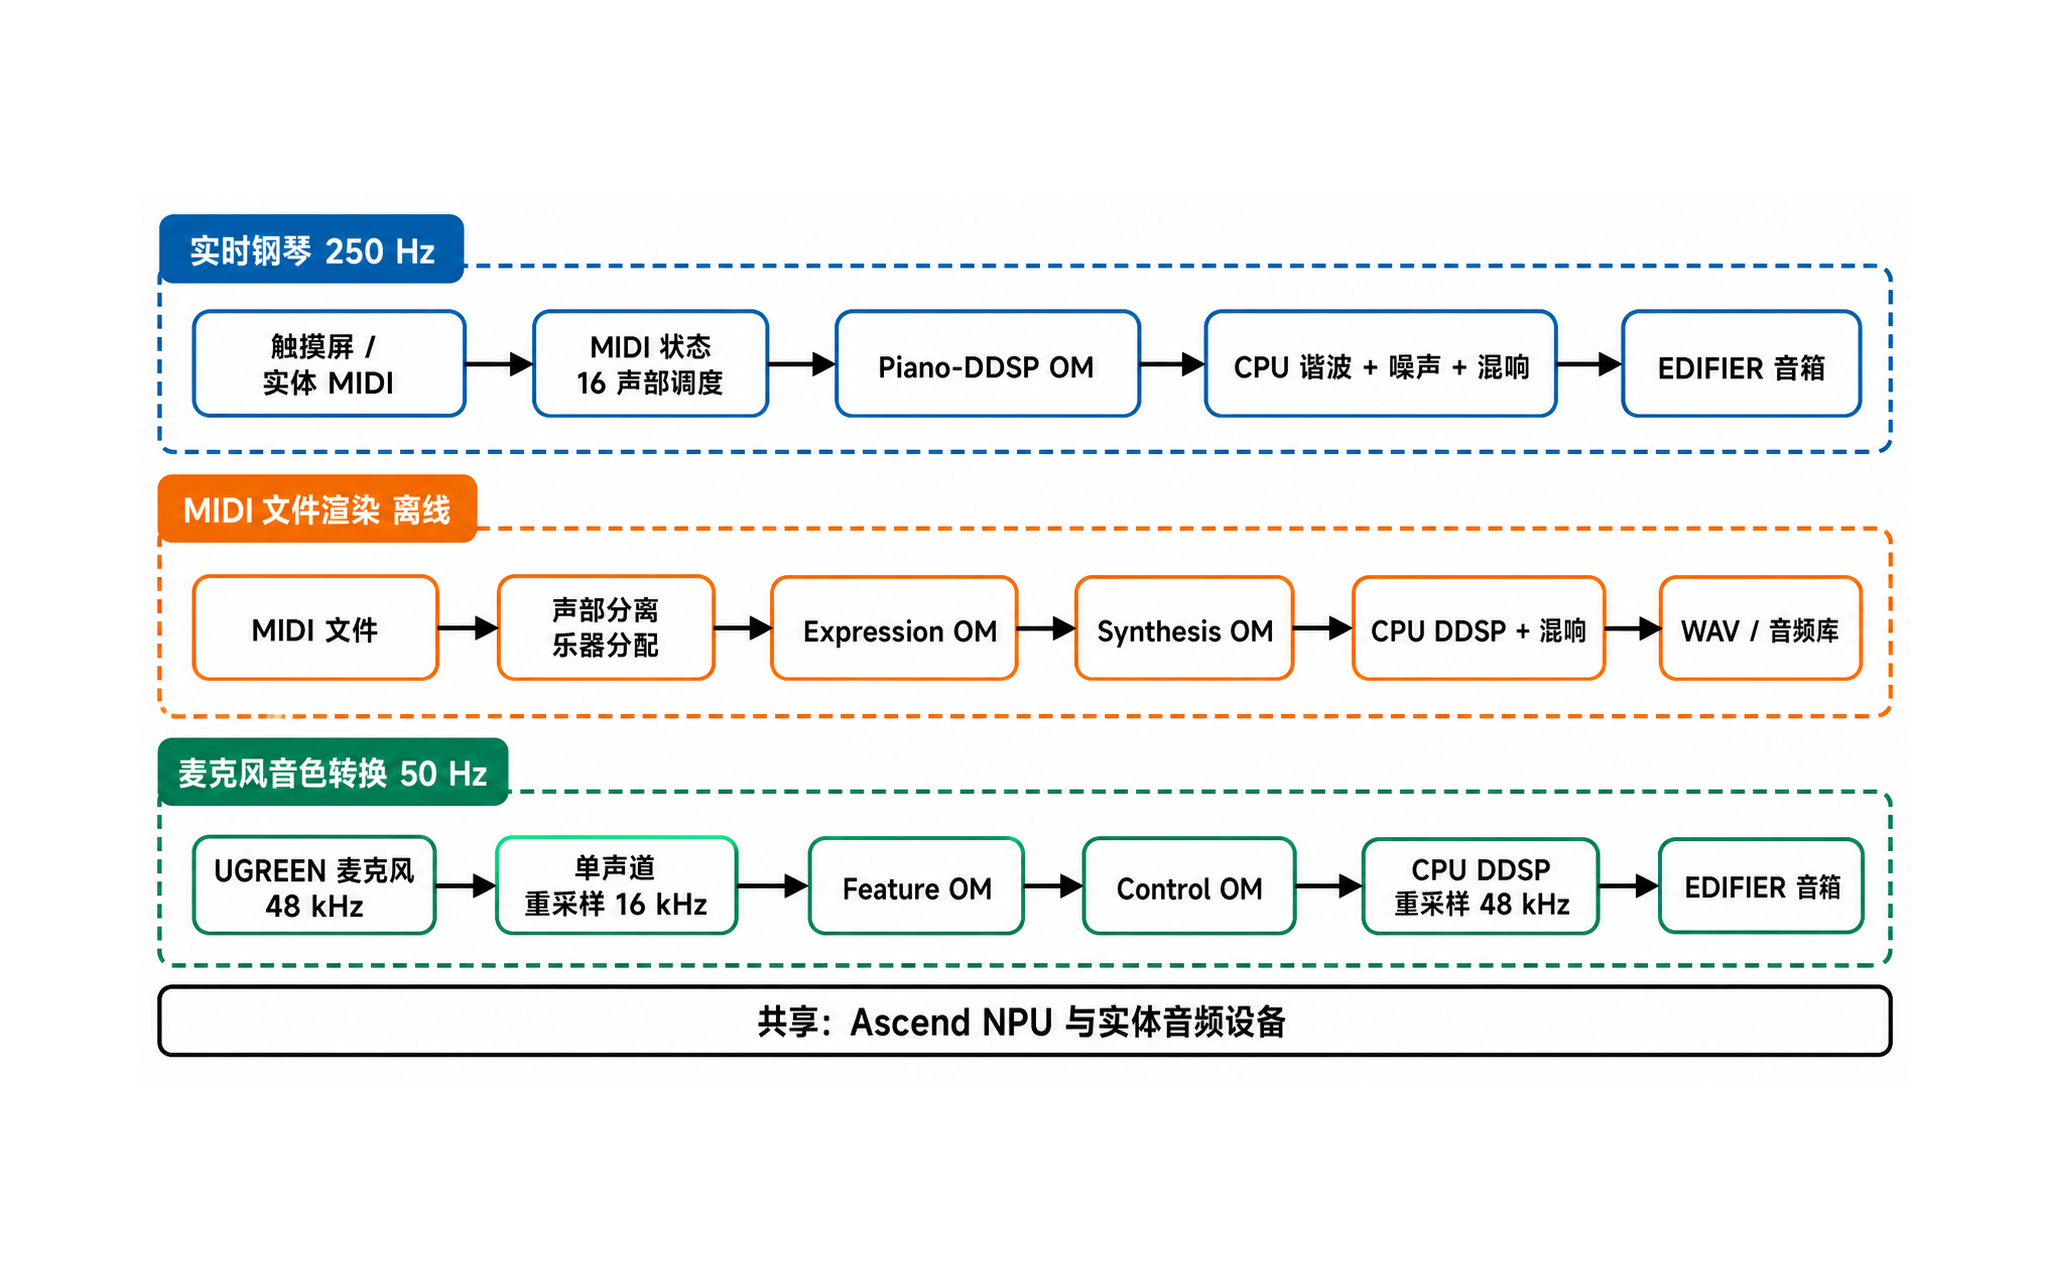
\includegraphics[keepaspectratio,alt={Case 3 的实时钢琴、MIDI 文件渲染和麦克风音色转换三条业务链}]{cases/img3/case3-three-workflows.png}}
\caption{Case 3 的实时钢琴、MIDI 文件渲染和麦克风音色转换三条业务链}
\end{figure}

三条链路共享 NPU 和音频设备，但时间模型不同。Piano-DDSP 每
\passthrough{\lstinline!4 ms!} 更新一次控制量；MIDI-DDSP
先知道完整乐曲并离线生成 WAV；DDSP-VST 每
\passthrough{\lstinline!20 ms!}
处理一帧音高和响度控制。它们不能被简单合并为一个``通用模型''。

\subsection{硬件连接}\label{src-experiment-case3-hardware-connection}

\begin{figure}
\centering
\pandocbounded{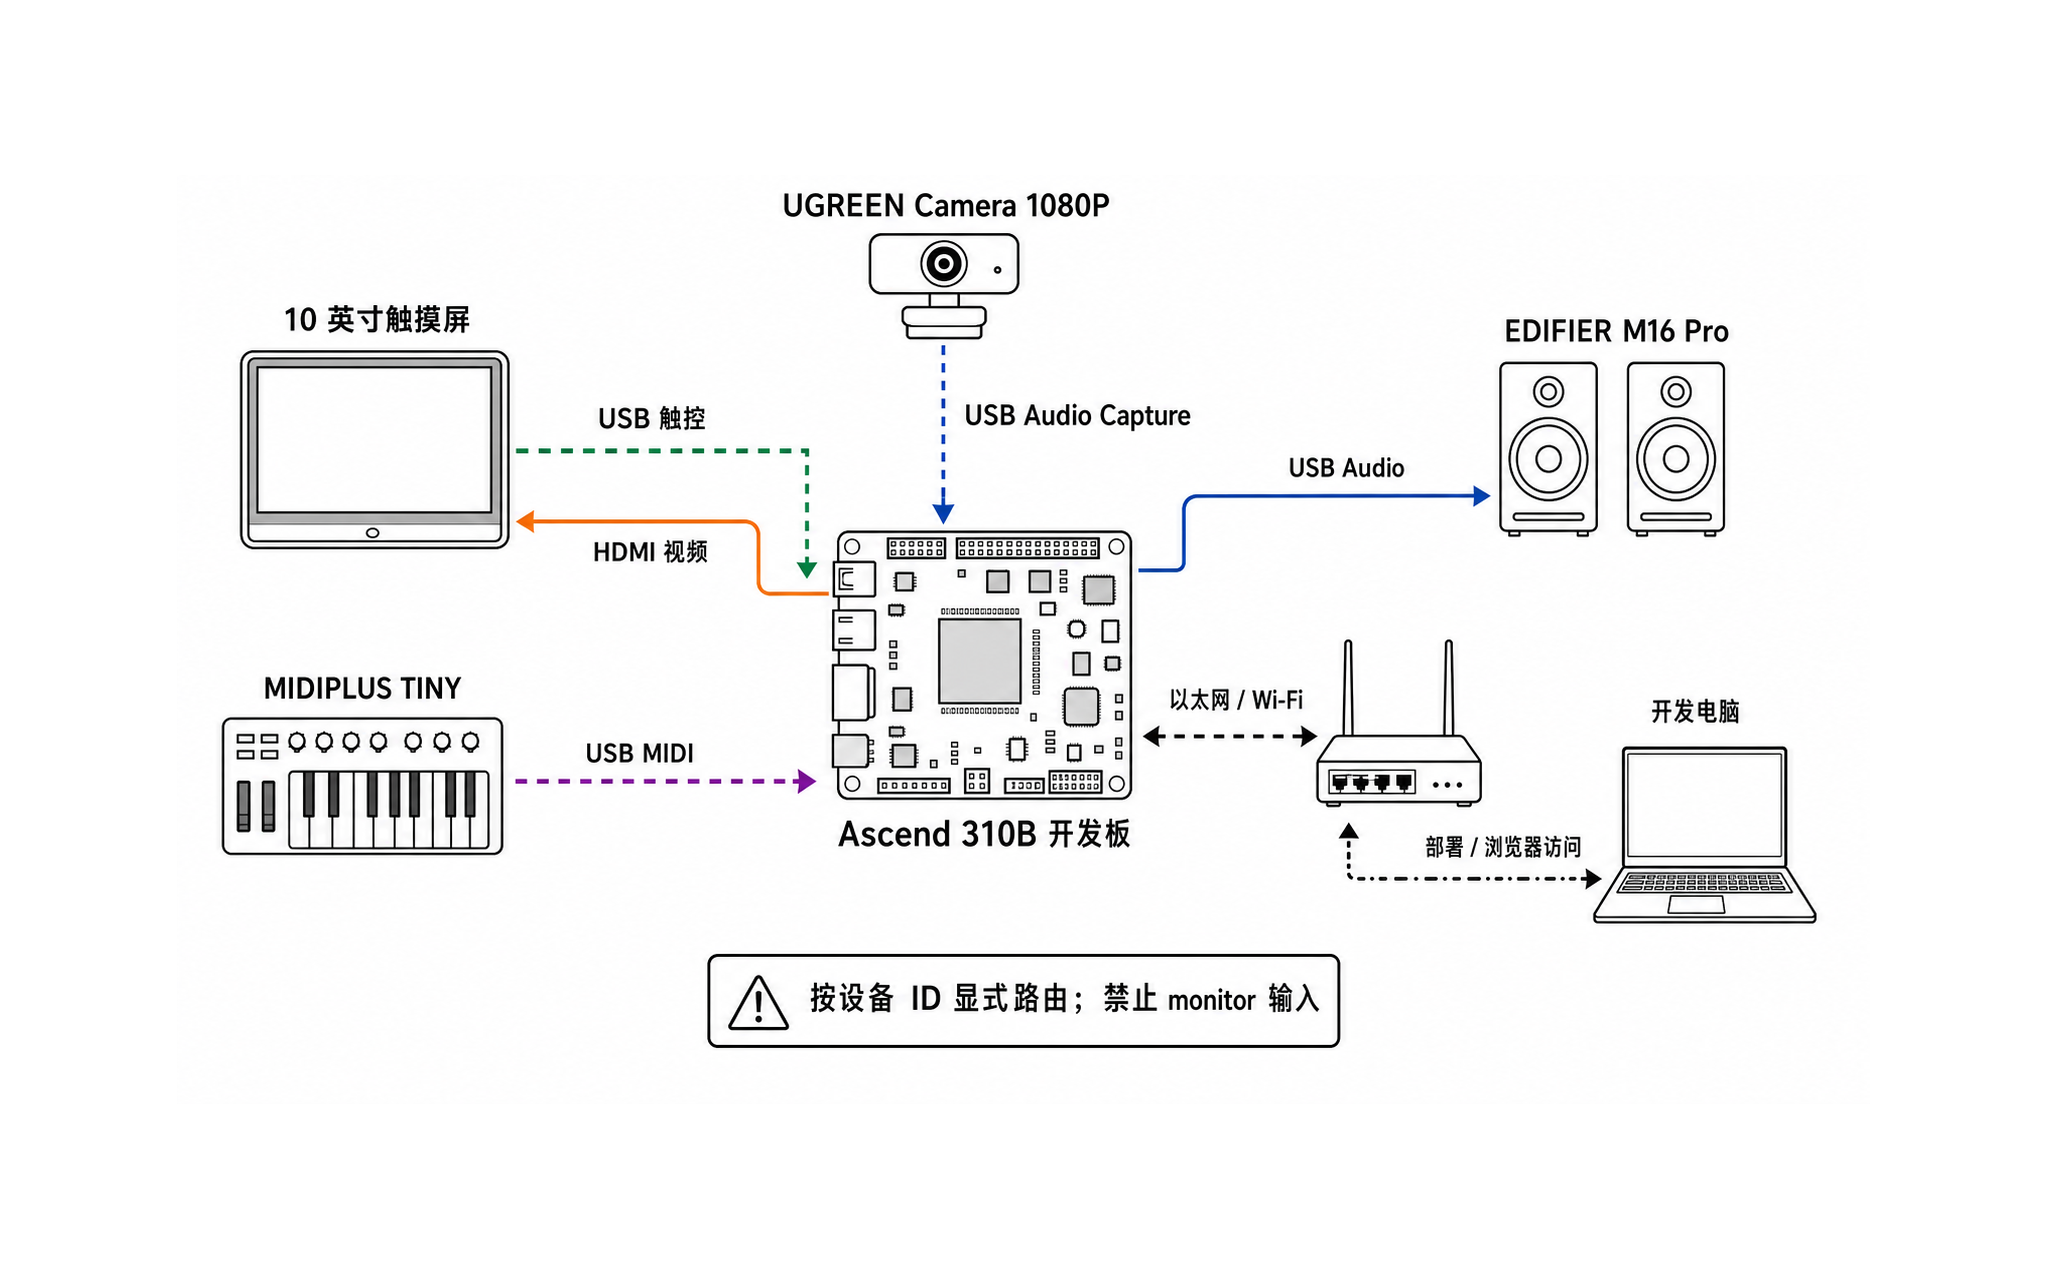
\includegraphics[keepaspectratio,alt={Ascend 310B 开发板与触摸屏、MIDI 键盘、USB 麦克风、音箱和开发电脑的硬件连接}]{cases/img3/case3-hardware-connections.png}}
\caption{Ascend 310B 开发板与触摸屏、MIDI 键盘、USB
麦克风、音箱和开发电脑的硬件连接}
\end{figure}

应按设备 ID
选择输入输出。程序不会在摄像头或音箱断开后静默切换到其他设备，也不会把
\passthrough{\lstinline!Monitor of ...!}
当作麦克风。这样的显式路由可以避免突然回放系统声音、产生反馈或把测试发到错误音箱。

\subsection{开发电脑与开发板的职责边界}\label{src-experiment-case3-runtime-boundary}

\begin{figure}
\centering
\pandocbounded{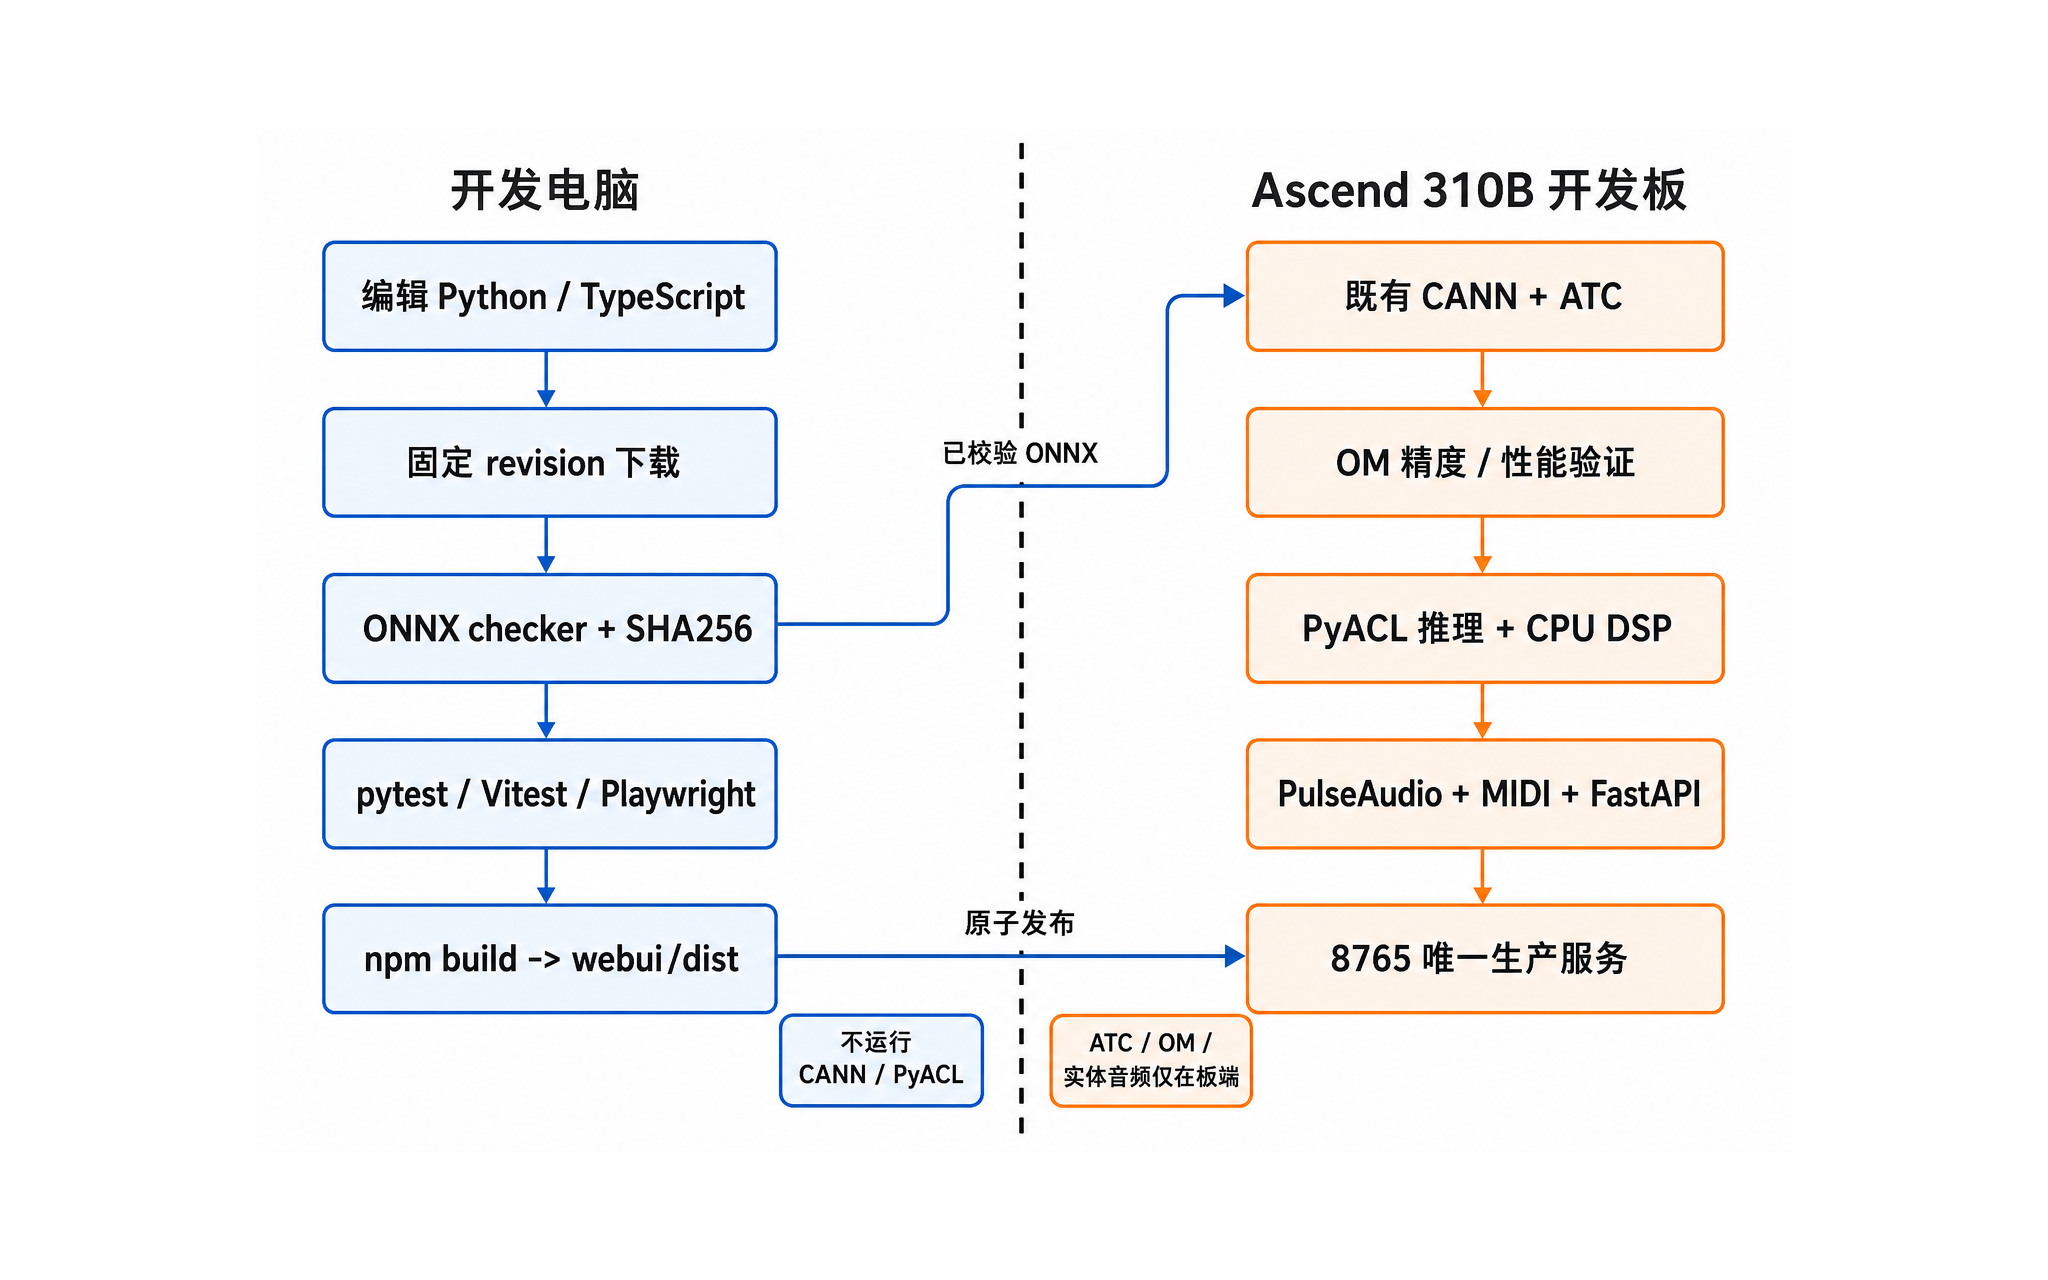
\includegraphics[keepaspectratio,alt={开发电脑与 Ascend 310B 开发板的职责边界}]{cases/img3/case3-runtime-boundary.png}}
\caption{开发电脑与 Ascend 310B 开发板的职责边界}
\end{figure}

{ % do not increment counter
\begin{longtable}[]{@{}lcc@{}}
\toprule\noalign{}
操作 & 开发电脑 & Ascend 310B \\
\midrule\noalign{}
\endhead
\bottomrule\noalign{}
\endlastfoot
编辑源码、运行普通 Python 单元测试 & 是 & 否 \\
\passthrough{\lstinline!npm ci!}、\passthrough{\lstinline!npm run test!}、\passthrough{\lstinline!npm run build!}
& 是 & 否 \\
下载并校验发布模型 & 是 & 可接收已校验资产 \\
TensorFlow/TFLite 历史导出 & 不属于 case3 当前流程 & 否 \\
ATC、PyACL、OM 推理、\passthrough{\lstinline!npu-smi!} & 否 & 是 \\
PulseAudio 实体路由和真实听音 & 否 & 是 \\
\end{longtable}
}

\section{4. DDSP 原理}\label{src-experiment-case3-ddsp-theory}

\subsection{从采样合成到可微分
DSP}\label{src-experiment-case3-ddsp-motivation}

传统采样合成器把大量录音映射到音高和力度区域，音色逼真但资产大，跨音高和连续控制依赖插值。端到端波形神经网络可以直接预测音频，却需要在音频采样率上输出大量数据，实时部署的计算量、状态和可解释性都更困难。

DDSP
将已知的振荡器、滤波器、包络和混响写成可微模块，训练时仍可通过梯度优化，部署时只让神经网络预测少量控制量。Google
的 DDSP 工作证明了这种``神经网络负责控制，DSP
负责生成''的音频建模方式。\href{https://arxiv.org/abs/2001.04643}{DDSP
论文}和\href{https://github.com/magenta/ddsp}{官方代码}给出了完整背景。

\subsection{基频、谐波和相位}\label{src-experiment-case3-harmonic-synthesis}

设采样率为 \(f_s\)，第 \(n\) 个采样的基频为 \(f_0[n]\)。第 \(k\)
个谐波的相位按下式累积：

\[
\phi_k[n+1] = \phi_k[n] + \frac{2\pi k f_0[n]}{f_s}.
\]

网络预测总幅度 \(A[n]\) 和未归一化谐波参数
\(z_k[n]\)。使用非负映射和归一化得到谐波比例：

\[
c_k[n] = \frac{\operatorname{softplus}(z_k[n])}
{\sum_{j=1}^{K}\operatorname{softplus}(z_j[n]) + \varepsilon}.
\]

谐波信号为：

\[
x_h[n] = A[n]\sum_{k=1}^{K}c_k[n]\sin(\phi_k[n]).
\]

超过奈奎斯特频率的谐波必须被抑制，即 \(k f_0[n] < f_s/2\)。Piano-DDSP
还预测
\passthrough{\lstinline!inharmonicity!}，用于表达钢琴弦的部分音偏离整数倍基频的现象。

\subsection{滤波噪声、包络、重采样和混响}\label{src-experiment-case3-noise-reverb}

噪声支路把白噪声 \(w[n]\) 变换到频域，并用网络预测的频带幅度 \(H_b[t]\)
构成时变滤波器：

\[
x_n[n] = \operatorname{ISTFT}\left(\operatorname{STFT}(w[n]) \odot H[t,f]\right).
\]

最终干声是谐波和噪声之和：

\[
x_{dry}[n] = g_h x_h[n] + g_n x_n[n].
\]

控制网络工作在 \passthrough{\lstinline!50 Hz!} 或
\passthrough{\lstinline!250 Hz!}，远低于
\passthrough{\lstinline!16 kHz!}
音频采样率，因此幅度、基频和频带系数需要插值到音频时间轴。混响可以是学习到的冲激响应
\(r[n]\)，也可以是 FreeVerb 风格反馈延迟网络：

\[
x_{wet}[n] = x_{dry}[n] * r[n], \qquad
y[n] = (1-m)x_{dry}[n] + m x_{wet}[n].
\]

\begin{figure}
\centering
\pandocbounded{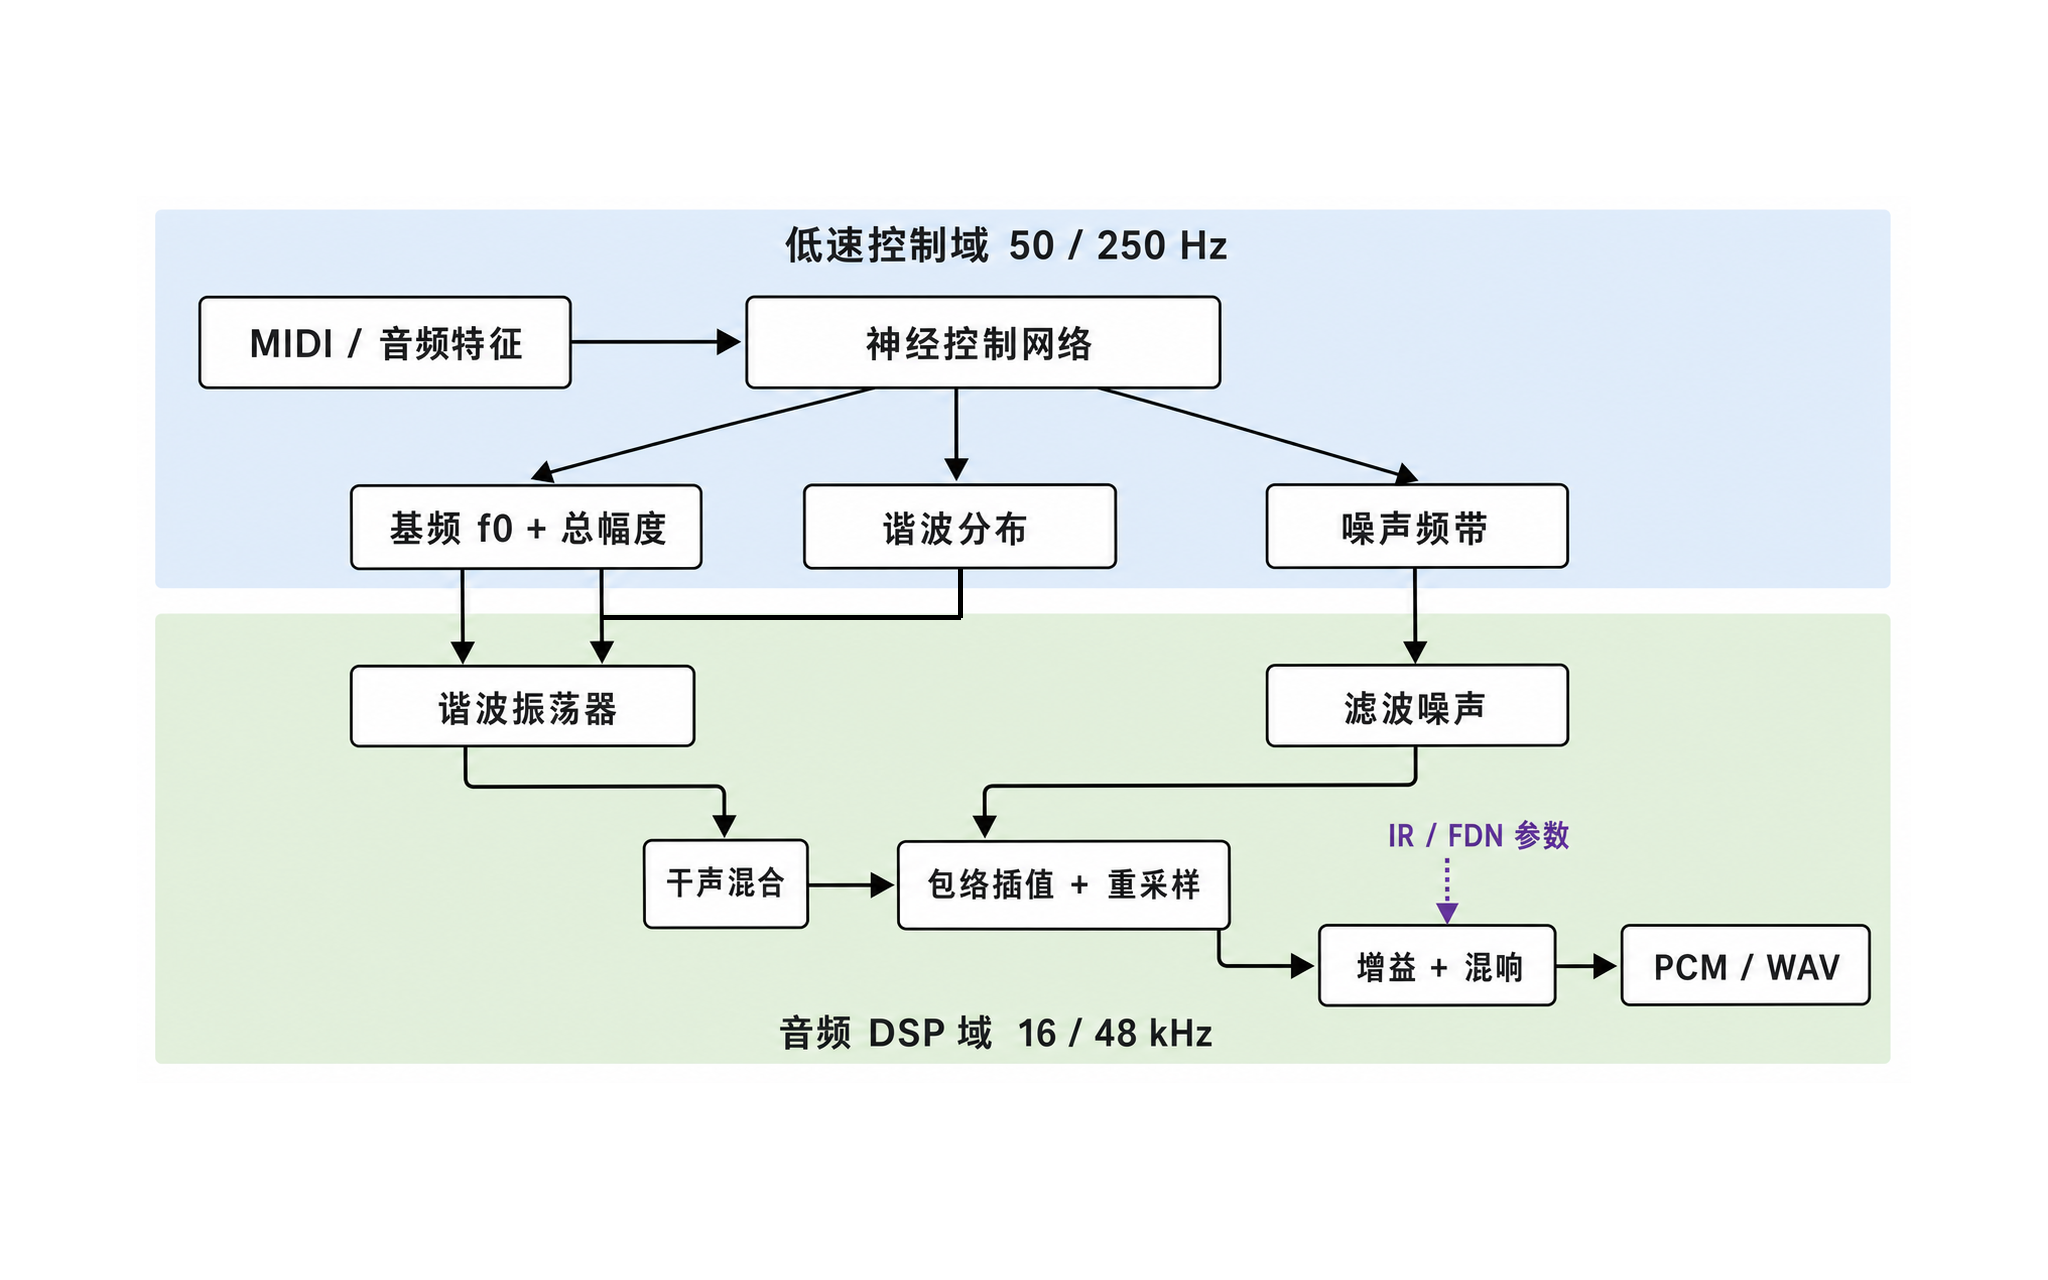
\includegraphics[keepaspectratio,alt={DDSP 从低速神经控制量到音频 DSP 输出的信号流程}]{cases/img3/case3-ddsp-synthesis-flow.png}}
\caption{DDSP 从低速神经控制量到音频 DSP 输出的信号流程}
\end{figure}

\subsection{参数如何改变听感}\label{src-experiment-case3-perception}

{ % do not increment counter
\begin{longtable}[]{@{}
  >{\raggedright\arraybackslash}p{(\linewidth - 4\tabcolsep) * \real{0.3333}}
  >{\raggedright\arraybackslash}p{(\linewidth - 4\tabcolsep) * \real{0.3333}}
  >{\raggedright\arraybackslash}p{(\linewidth - 4\tabcolsep) * \real{0.3333}}@{}}
\toprule\noalign{}
\begin{minipage}[b]{\linewidth}\raggedright
控制量
\end{minipage} & \begin{minipage}[b]{\linewidth}\raggedright
物理或听觉含义
\end{minipage} & \begin{minipage}[b]{\linewidth}\raggedright
常见异常
\end{minipage} \\
\midrule\noalign{}
\endhead
\bottomrule\noalign{}
\endlastfoot
\passthrough{\lstinline!f0!} & 基频，决定音高和滑音轨迹 &
噪声被误检为基频时会出现无意义的低音或抖动 \\
幅度或响度 & 控制音符包络和整体强弱 &
过大会削波，过小会让音色模型看不到有效输入 \\
谐波分布 & 决定明亮度、共鸣和乐器主体音色 &
高频谐波过多会尖锐，归一化错误会改变总能量 \\
噪声频带 & 表达吹气、摩擦、击弦和瞬态 &
过高会产生嘶声，全部关闭会让音色不自然 \\
混响 & 表达空间和尾音 & 全湿声会掩盖起音，实时链路中也会增加主观拖尾 \\
噪声门 & 阻止环境底噪触发模型 &
阈值过低会持续触发，过高会吞掉轻声起音 \\
\end{longtable}
}

\section{5.
三套神经网络架构}\label{src-experiment-case3-model-architectures}

\subsection{Piano-DDSP}\label{src-experiment-case3-piano-ddsp}

当前发布为 \passthrough{\lstinline!model-suite-v1.0.1!}，模型结构源自
\href{https://github.com/lrenault/ddsp-piano}{DDSP-Piano}：\passthrough{\lstinline!16 kHz!}
音频、\passthrough{\lstinline!250 Hz!} 控制率、每次一帧、每帧
\passthrough{\lstinline!64!} 个采样、最多 \passthrough{\lstinline!16!}
个声部。部署图显式输入和输出循环状态，开发板激活的 bundle 为
\passthrough{\lstinline!model-suite-v1.0.1-gru-unrolled-fp32-origin!}，默认模型为
\passthrough{\lstinline!gru\_ir\_96\_64!}。GRU
被展开为基础算子，以适配当前 \passthrough{\lstinline!Ascend310B4!} 的
FP32 编译和连续状态验证。

\begin{figure}
\centering
\pandocbounded{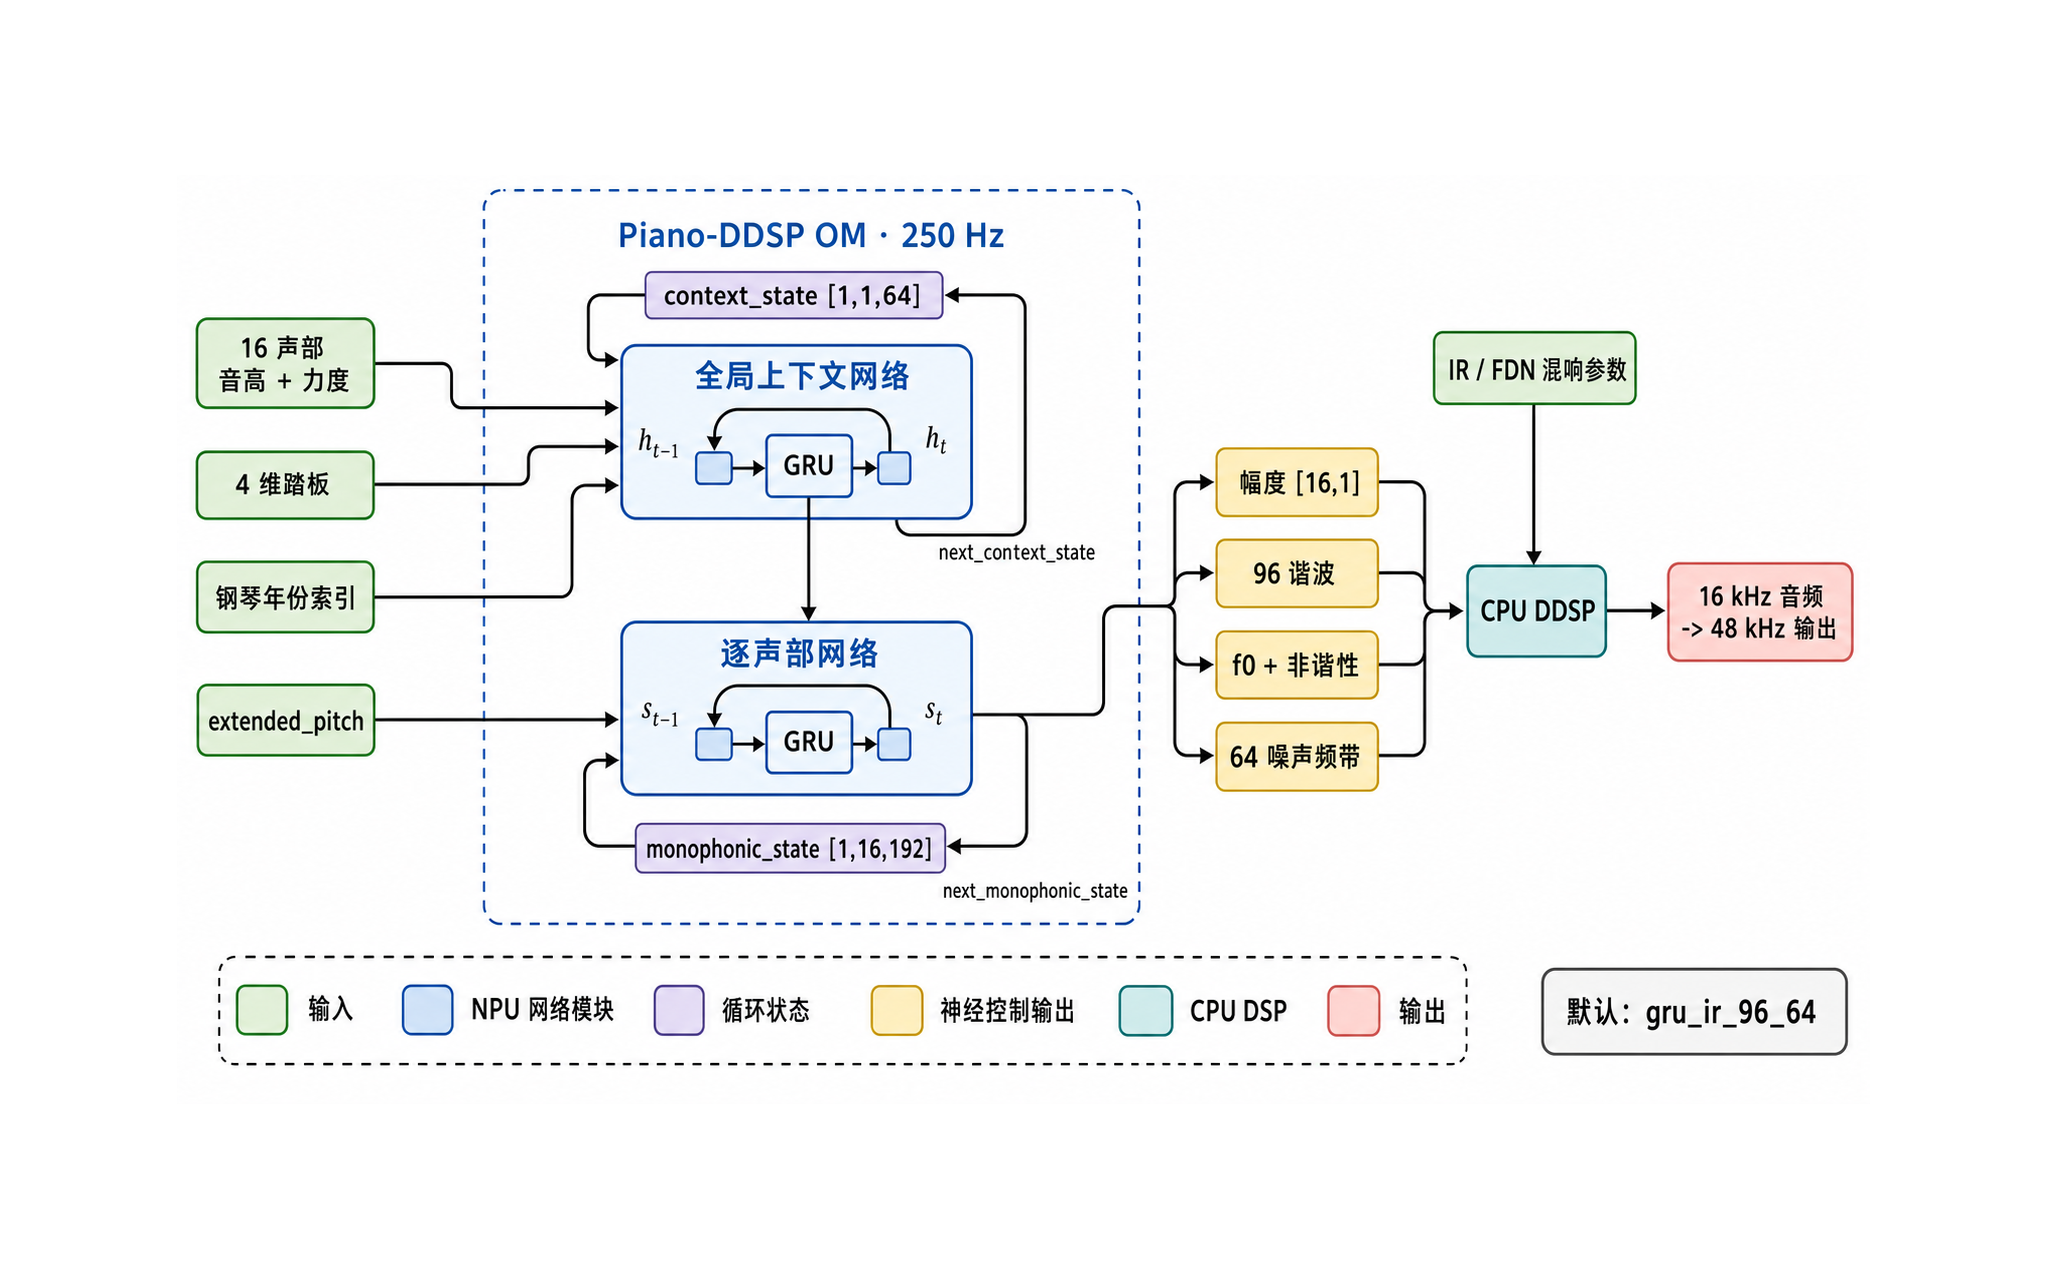
\includegraphics[keepaspectratio,alt={Piano-DDSP 的上下文网络、逐声部网络、循环状态和 CPU 合成边界}]{cases/img3/case3-piano-ddsp-architecture.png}}
\caption{Piano-DDSP 的上下文网络、逐声部网络、循环状态和 CPU 合成边界}
\end{figure}

主要张量合同如下，所有张量均为 FP32：

{ % do not increment counter
\begin{longtable}[]{@{}llll@{}}
\toprule\noalign{}
方向 & 张量 & 形状 & 含义 \\
\midrule\noalign{}
\endhead
\bottomrule\noalign{}
\endlastfoot
输入 & \passthrough{\lstinline!conditioning!} &
\passthrough{\lstinline![1,1,16,2]!} & 16 声部的音高与力度条件 \\
输入 & \passthrough{\lstinline!pedal!} &
\passthrough{\lstinline![1,1,4]!} & 踏板与连续控制状态 \\
输入 & \passthrough{\lstinline!piano\_model!} &
\passthrough{\lstinline![1]!} & MAESTRO 钢琴年份索引 \\
输入 & \passthrough{\lstinline!extended\_pitch!} &
\passthrough{\lstinline![1,1,16,1]!} & 扩展音高条件 \\
输入 & \passthrough{\lstinline!context\_state!} &
\passthrough{\lstinline![1,1,64]!} & 全局循环状态 \\
输入 & \passthrough{\lstinline!monophonic\_state!} &
\passthrough{\lstinline![1,16,192]!} & 每声部循环状态 \\
输出 & \passthrough{\lstinline!amplitudes!} &
\passthrough{\lstinline![1,1,16,1]!} & 声部总幅度 \\
输出 & \passthrough{\lstinline!harmonic\_distribution!} &
\passthrough{\lstinline![1,1,16,96]!} & 96 个谐波比例 \\
输出 &
\passthrough{\lstinline!inharmonicity!}、\passthrough{\lstinline!f0\_hz!}
& \passthrough{\lstinline![1,1,16,1]!} & 非谐性和基频 \\
输出 & \passthrough{\lstinline!noise\_magnitudes!} &
\passthrough{\lstinline![1,1,16,64]!} & 64 个噪声频带 \\
输出 & \passthrough{\lstinline!reverb\_ir!} &
\passthrough{\lstinline![1,24000]!} & 学习到的混响冲激响应 \\
输出 & \passthrough{\lstinline!next\_context\_state!} &
\passthrough{\lstinline![1,1,64]!} & 下一帧全局状态 \\
输出 & \passthrough{\lstinline!next\_monophonic\_state!} &
\passthrough{\lstinline![1,16,192]!} & 下一帧声部状态 \\
\end{longtable}
}

四个已发布候选模型都通过 \passthrough{\lstinline!10,000!} 帧 OM
连续对照，但结构和混响边界不同：

{ % do not increment counter
\begin{longtable}[]{@{}lllll@{}}
\toprule\noalign{}
变体 & 时序调制 & 混响 & 谐波/噪声 & 当前作用 \\
\midrule\noalign{}
\endhead
\bottomrule\noalign{}
\endlastfoot
GRU IR & GRU & 学习 IR & 96/64 & 当前默认激活模型 \\
FiLM FDN & FiLM & FDN & 128/96 & 可配置候选 \\
GRU 全湿声 & GRU & 全湿声 IR & 96/64 & 感知校准候选 \\
FiLM 全湿声 & FiLM & 全湿声 IR & 96/64 & FiLM 与学习 IR 候选 \\
\end{longtable}
}

清单中的完整模型 ID 为：

\begin{lstlisting}
gru_ir_96_64
film_fdn_128_96
gru_ir_fullwet_96_64
film_ir_fullwet_96_64
\end{lstlisting}

\subsection{MIDI-DDSP}\label{src-experiment-case3-midi-ddsp}

\begin{figure}[H]
\centering
\pandocbounded{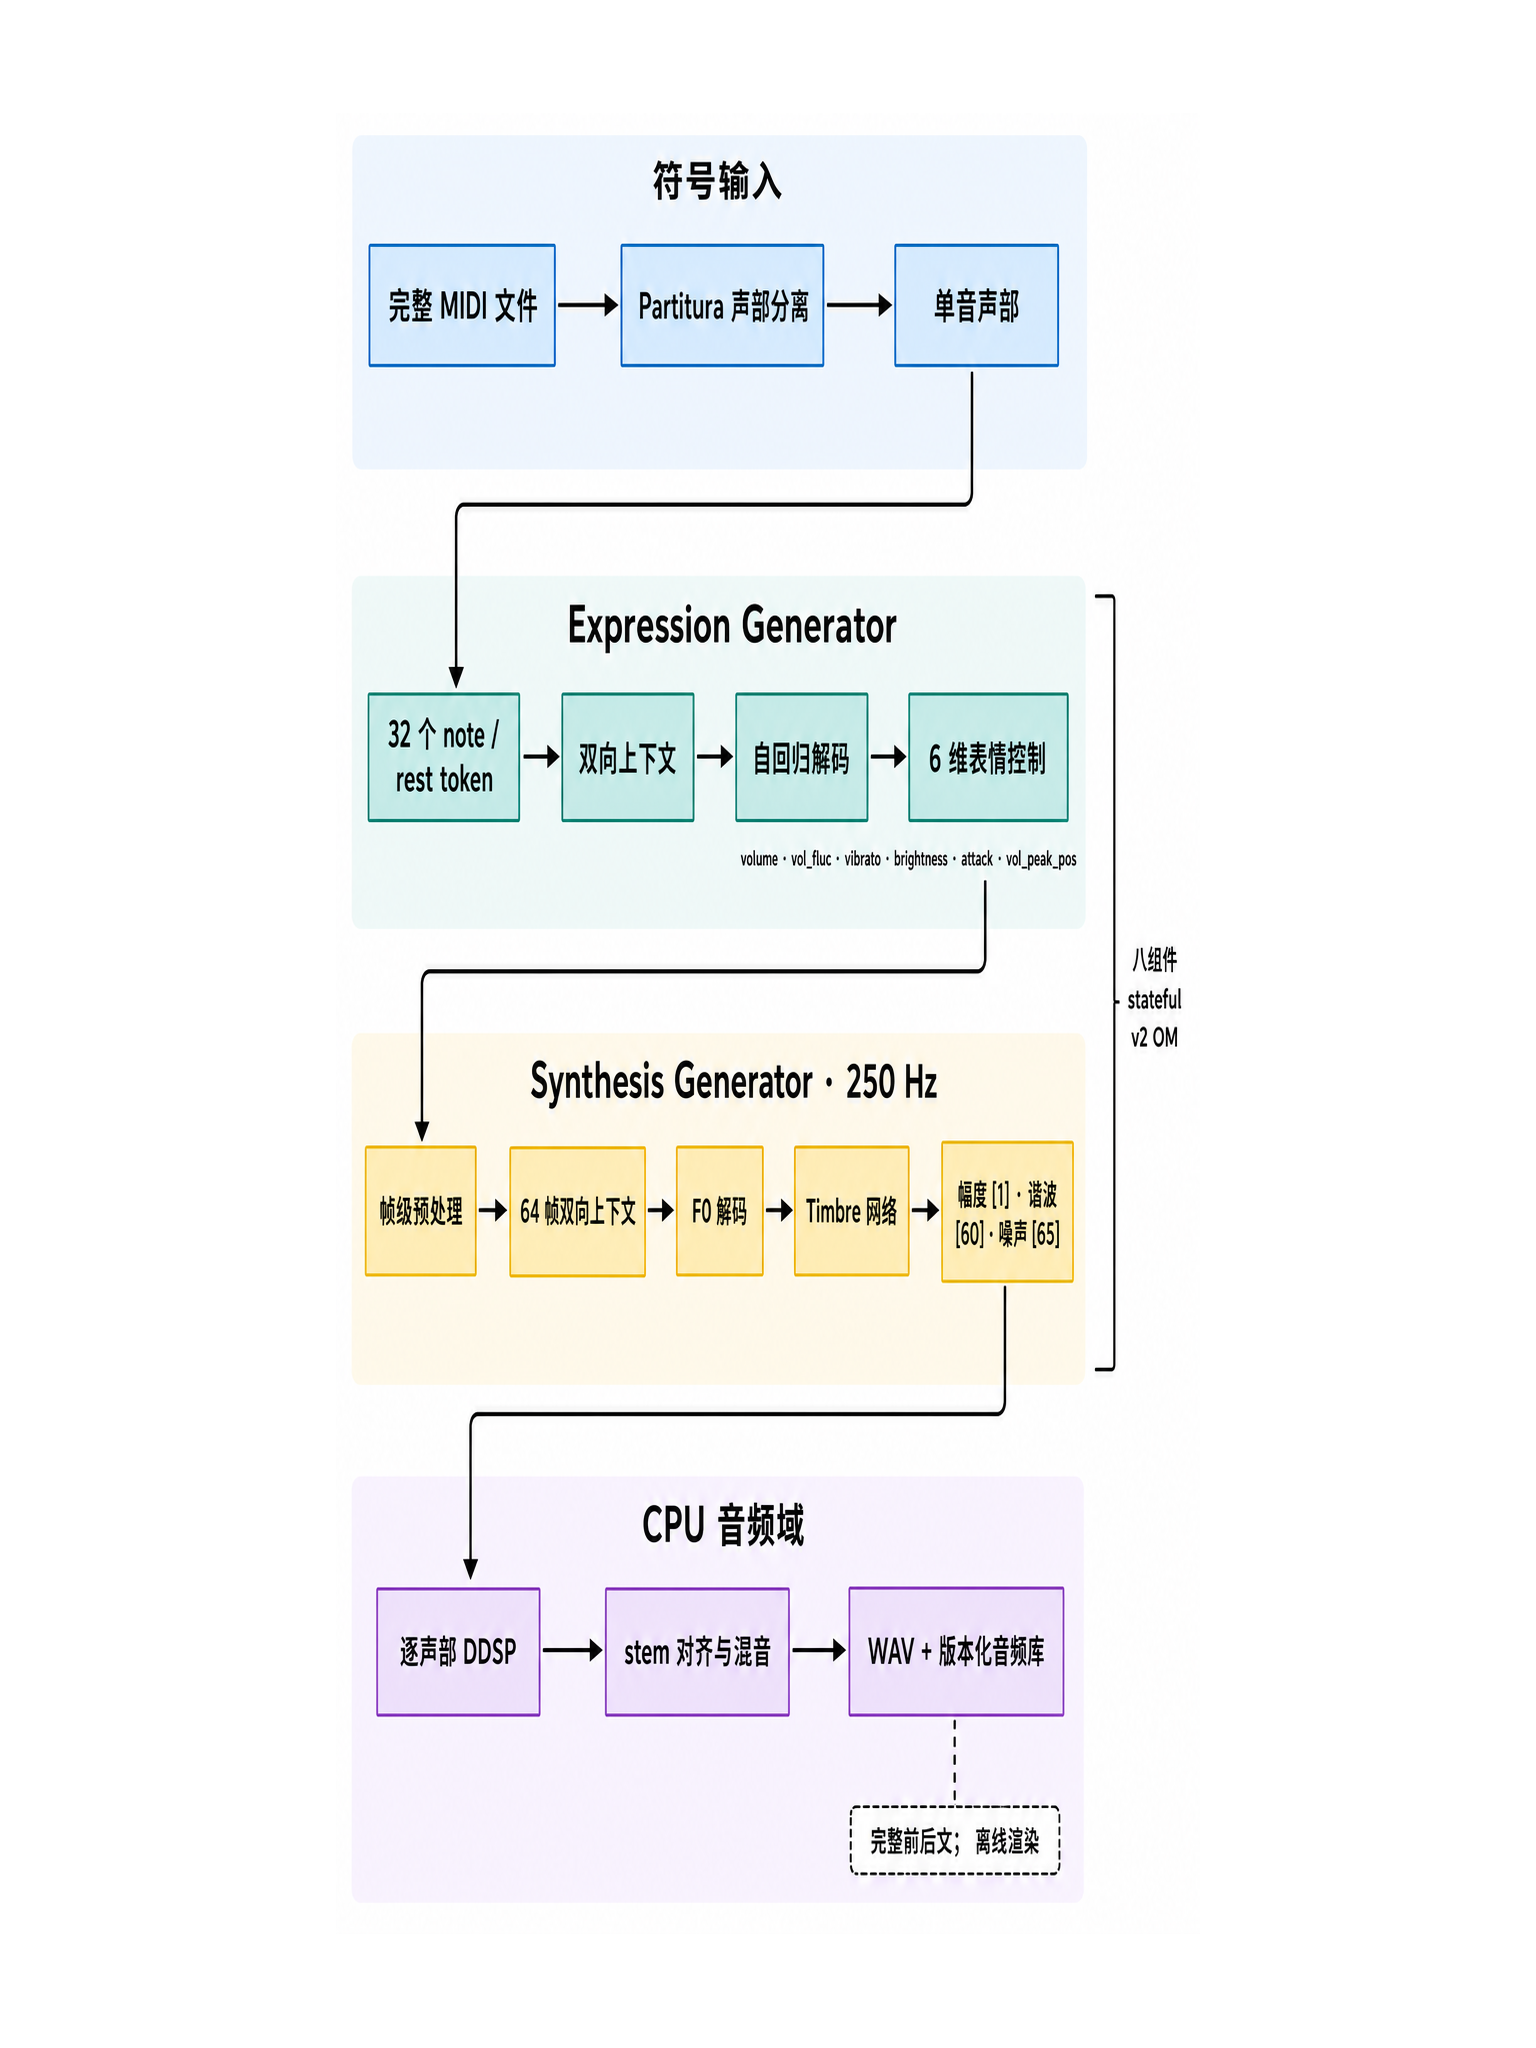
\includegraphics[keepaspectratio,alt={MIDI-DDSP 从符号输入、Expression Generator、Synthesis Generator 到 CPU 音频域的层级结构}]{cases/img3/case3-midi-ddsp-architecture.png}}
\caption{MIDI-DDSP 从符号输入、Expression Generator、Synthesis Generator
到 CPU 音频域的层级结构}
\end{figure}

MIDI-DDSP 为已知完整乐曲的离线层级模型，不是物理 MIDI
键盘的低延迟模型。Expression Generator 先从最长
\passthrough{\lstinline!32!} 个 note/rest token 的上下文预测
\passthrough{\lstinline!6!}
维表情控制：\passthrough{\lstinline!volume!}、\passthrough{\lstinline!vol\_fluc!}、\passthrough{\lstinline!vibrato!}、\passthrough{\lstinline!brightness!}、\passthrough{\lstinline!attack!}
和 \passthrough{\lstinline!vol\_peak\_pos!}。Synthesis Generator 再用
\passthrough{\lstinline!64!} 帧窗口、\passthrough{\lstinline!250 Hz!}
控制率生成音频控制量。\href{https://openreview.net/forum?id=UseMOjWENv}{MIDI-DDSP
论文}和\href{https://github.com/magenta/midi-ddsp}{官方仓库}解释了这种符号控制与音色合成的层级结构。

stateful v2 把原始图拆成八个可独立转换和批处理的组件：

{ % do not increment counter
\begin{longtable}[]{@{}
  >{\raggedright\arraybackslash}p{(\linewidth - 2\tabcolsep) * \real{0.5000}}
  >{\raggedright\arraybackslash}p{(\linewidth - 2\tabcolsep) * \real{0.5000}}@{}}
\toprule\noalign{}
\begin{minipage}[b]{\linewidth}\raggedright
组件
\end{minipage} & \begin{minipage}[b]{\linewidth}\raggedright
关键输入输出
\end{minipage} \\
\midrule\noalign{}
\endhead
\bottomrule\noalign{}
\endlastfoot
\passthrough{\lstinline!expression\_context\_forward!} & 前向 token
上下文与状态 \\
\passthrough{\lstinline!expression\_context\_backward!} & 反向 token
上下文与状态 \\
\passthrough{\lstinline!expression\_decode!} &
上下文、上一控制与下一自回归状态 \\
\passthrough{\lstinline!synthesis\_precondition!} &
帧级音高、表情和乐器条件 \\
\passthrough{\lstinline!synthesis\_context\_forward!} &
前向帧上下文与状态 \\
\passthrough{\lstinline!synthesis\_context\_backward!} &
反向帧上下文与状态 \\
\passthrough{\lstinline!synthesis\_f0\_decode!} & 基频控制与解码状态 \\
\passthrough{\lstinline!synthesis\_timbre!} &
\passthrough{\lstinline!amplitude[1]!}、\passthrough{\lstinline!harmonics[60]!}、\passthrough{\lstinline!noise\_amps[65]!} \\
\end{longtable}
}

模型为单声部建模。程序先把 MIDI 分成单音声部，再按静态 batch
\passthrough{\lstinline!1/2/4/8!} 选择最小可容纳 OM，生成每个
stem，最后对齐并混音。双向上下文需要看到完整前后文，因此不能把这条链路直接放到按键后的
\passthrough{\lstinline!4 ms!} 实时路径中。

\subsection{DDSP-VST Feature 与
Control}\label{src-experiment-case3-ddsp-vst}

DDSP-VST Effect
参考\href{https://github.com/magenta/ddsp-vst/tree/f2996e97f9469f3956a6b8e9d2d9b50b6555e1e9}{固定上游提交
\passthrough{\lstinline!f2996e97!}}。Feature 模型来自
\passthrough{\lstinline!extract\_features\_micro.tflite!}。固定上游提交的完整值为：

\begin{lstlisting}
f2996e97f9469f3956a6b8e9d2d9b50b6555e1e9
\end{lstlisting}

Feature 源码 SHA256 为：

\begin{lstlisting}
98ade06772f9ca6ac64789fd843f14aeddf709084bbc76f060761b141837d0a2
\end{lstlisting}

case3 只保留验证后的 ONNX、OM 和转换证据，不保留 TFLite 导出工具。当前
Feature OM 使用 \passthrough{\lstinline!mixed\_float16!}，Control OM
对应选择的乐器音色。

\begin{figure}
\centering
\pandocbounded{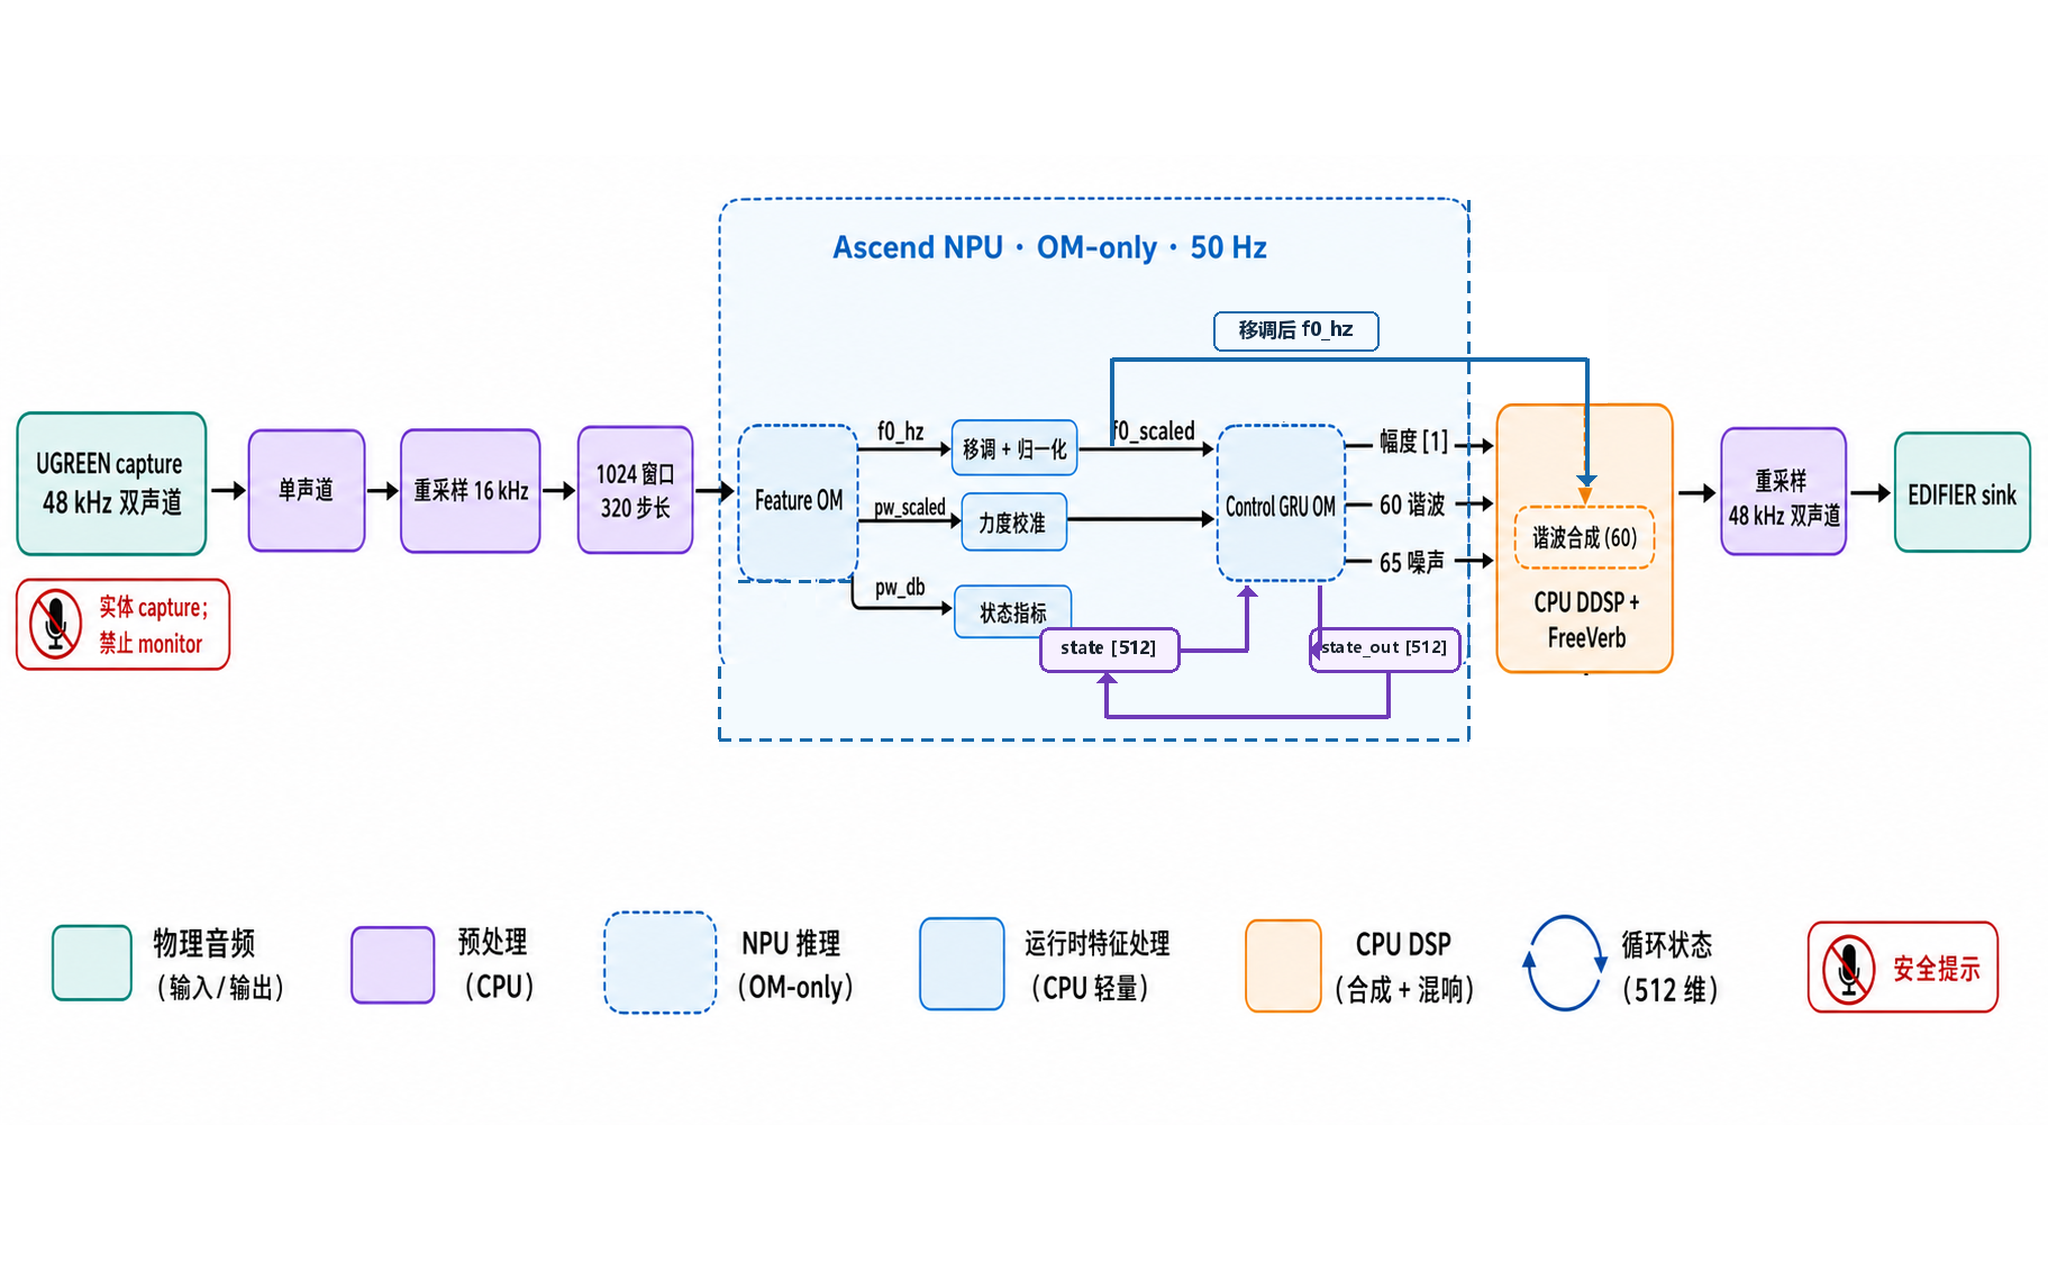
\includegraphics[keepaspectratio,alt={DDSP-VST Effect 的实体音频输入、Feature OM、Control GRU 状态回路和 CPU 音频输出}]{cases/img3/case3-ddsp-vst-architecture.png}}
\caption{DDSP-VST Effect 的实体音频输入、Feature OM、Control GRU
状态回路和 CPU 音频输出}
\end{figure}

{ % do not increment counter
\begin{longtable}[]{@{}
  >{\raggedright\arraybackslash}p{(\linewidth - 6\tabcolsep) * \real{0.2500}}
  >{\raggedright\arraybackslash}p{(\linewidth - 6\tabcolsep) * \real{0.2500}}
  >{\raggedright\arraybackslash}p{(\linewidth - 6\tabcolsep) * \real{0.2500}}
  >{\raggedright\arraybackslash}p{(\linewidth - 6\tabcolsep) * \real{0.2500}}@{}}
\toprule\noalign{}
\begin{minipage}[b]{\linewidth}\raggedright
模型
\end{minipage} & \begin{minipage}[b]{\linewidth}\raggedright
输入
\end{minipage} & \begin{minipage}[b]{\linewidth}\raggedright
输出
\end{minipage} & \begin{minipage}[b]{\linewidth}\raggedright
时率与作用
\end{minipage} \\
\midrule\noalign{}
\endhead
\bottomrule\noalign{}
\endlastfoot
Feature OM & \passthrough{\lstinline!float32[1024]!} 音频 &
\passthrough{\lstinline!f0\_scaled[1]!}、\passthrough{\lstinline!pw\_scaled[1]!}、\passthrough{\lstinline!f0\_hz[1]!}、\passthrough{\lstinline!pw\_db[1]!}
& \passthrough{\lstinline!16 kHz!}，步长
\passthrough{\lstinline!320!}，即 \passthrough{\lstinline!50 Hz!} \\
Control OM &
\passthrough{\lstinline!state[512]!}、\passthrough{\lstinline!f0\_scaled[1]!}、\passthrough{\lstinline!pw\_scaled[1]!}
&
\passthrough{\lstinline!amplitude[1]!}、\passthrough{\lstinline!harmonics[60]!}、\passthrough{\lstinline!noise\_amps[65]!}、\passthrough{\lstinline!state\_out[512]!}
& 每 \passthrough{\lstinline!20 ms!} 更新音色控制与 GRU 状态 \\
\end{longtable}
}

控制目录包含
Bassoon、Clarinet、Flute、Melodica、Saxophone、Sitar、Trombone、Trumpet、Tuba、Violin
和 Vowels 共 11 种音色。界面显示中文乐器名，但模型
ID、清单和哈希仍保留稳定英文标识。

\subsection{三套网络对比}\label{src-experiment-case3-model-comparison}

{ % do not increment counter
\begin{longtable}[]{@{}
  >{\raggedright\arraybackslash}p{(\linewidth - 6\tabcolsep) * \real{0.2500}}
  >{\raggedright\arraybackslash}p{(\linewidth - 6\tabcolsep) * \real{0.2500}}
  >{\raggedright\arraybackslash}p{(\linewidth - 6\tabcolsep) * \real{0.2500}}
  >{\raggedright\arraybackslash}p{(\linewidth - 6\tabcolsep) * \real{0.2500}}@{}}
\toprule\noalign{}
\begin{minipage}[b]{\linewidth}\raggedright
特性
\end{minipage} & \begin{minipage}[b]{\linewidth}\raggedright
Piano-DDSP
\end{minipage} & \begin{minipage}[b]{\linewidth}\raggedright
MIDI-DDSP
\end{minipage} & \begin{minipage}[b]{\linewidth}\raggedright
DDSP-VST Effect
\end{minipage} \\
\midrule\noalign{}
\endhead
\bottomrule\noalign{}
\endlastfoot
输入 & MIDI 帧、踏板、钢琴索引 & 完整 MIDI 文件与乐器分配 &
实体麦克风音频 \\
主要用途 & 实时复音钢琴 & 离线高质量 MIDI 渲染 & 实时单音音色转换 \\
复音能力 & 固定 16 声部 & 分离后逐单音声部渲染并混音 & 单音输入 \\
控制率 & 250 Hz & 250 Hz & 50 Hz \\
时序状态 & 显式全局与逐声部状态 & 八组件双向和自回归状态 & 512 维
Control GRU 状态 \\
前后文 & 只依赖过去和当前帧 & 使用完整乐曲的双向上下文 &
滑动音频窗口与过去状态 \\
NPU 输出 & 96 谐波、64 噪声等控制 & 60 谐波、65 噪声等控制 & Feature
特征和 60/65 控制 \\
DSP 边界 & CPU 合成、重采样和 IR/FDN & CPU 合成、混响、stem 混音和 WAV &
CPU 合成、重采样、增益和 FreeVerb \\
\end{longtable}
}

\section{6. 模型获取与 Ascend
部署}\label{src-experiment-case3-model-deployment}

\subsection{只消费已发布模型}\label{src-experiment-case3-model-download}

case3 不再提供 TensorFlow、Keras、SavedModel 或 TFLite 到 ONNX
的导出代码。历史 TensorFlow/MIDI-DDSP
的模型结构、张量合同和验证过程仍保留在\href{https://github.com/zhouxzh/Ascend310/blob/main/samples/case3/doc/midi-ddsp-export.md}{历史导出文档}，但不再作为当前复现步骤。

当前下载入口为
\href{https://github.com/zhouxzh/Ascend310/blob/main/samples/case3/tools/download_model_release.py}{\passthrough{\lstinline!tools/download\_model\_release.py!}}。下载器拒绝
\passthrough{\lstinline!main!}、\passthrough{\lstinline!master!} 和
\passthrough{\lstinline!HEAD!} 等移动分支，先解析固定 revision，再下载
\passthrough{\lstinline!SHA256SUMS!}，支持
\passthrough{\lstinline!.part!}
断点续传，并在原子替换前逐文件验证。Piano-DDSP
\passthrough{\lstinline!model-suite-v1.0.1!} 的示例为：

\begin{lstlisting}
cd D:\Github\Ascend310\samples\case3
python tools/download_model_release.py `
  --revision model-suite-v1.0.1 `
  --manifest-sha256 1a4a2500ae357577a4a6f7378c28d54235f543663b9b69cc3cf5938929c458d7 `
  --target-dir models/piano_ddsp/model-suite-v1.0.1
\end{lstlisting}

发布仓库为
\href{https://huggingface.co/zhouxzh/piano-ddsp-ascend310}{\passthrough{\lstinline!zhouxzh/piano-ddsp-ascend310!}}。下载完成后还要核对解析出的固定提交（完整
SHA）：

\begin{lstlisting}
c41911aa7de454aeacf0b3edbb2d06a0801fb3ff
\end{lstlisting}

如果 revision、清单摘要或任一资产哈希不一致，应停止，不得继续 ATC。

DDSP-VST Feature 当前本地 release 已保存 ONNX、参考 NPZ、许可证、ATC
原始日志、两种精度验证和 SHA256；在新的不可变 HF revision
完成发布之前，不应把本地目录描述成已公开下载的
release。模型发布状态和操作以\href{https://github.com/zhouxzh/Ascend310/blob/main/samples/case3/doc/om-deployment.md}{模型与
OM 部署文档}为准。

\subsection{ONNX、ATC、OM 与 PyACL
验证链}\label{src-experiment-case3-atc-pipeline}

\begin{figure}
\centering
\pandocbounded{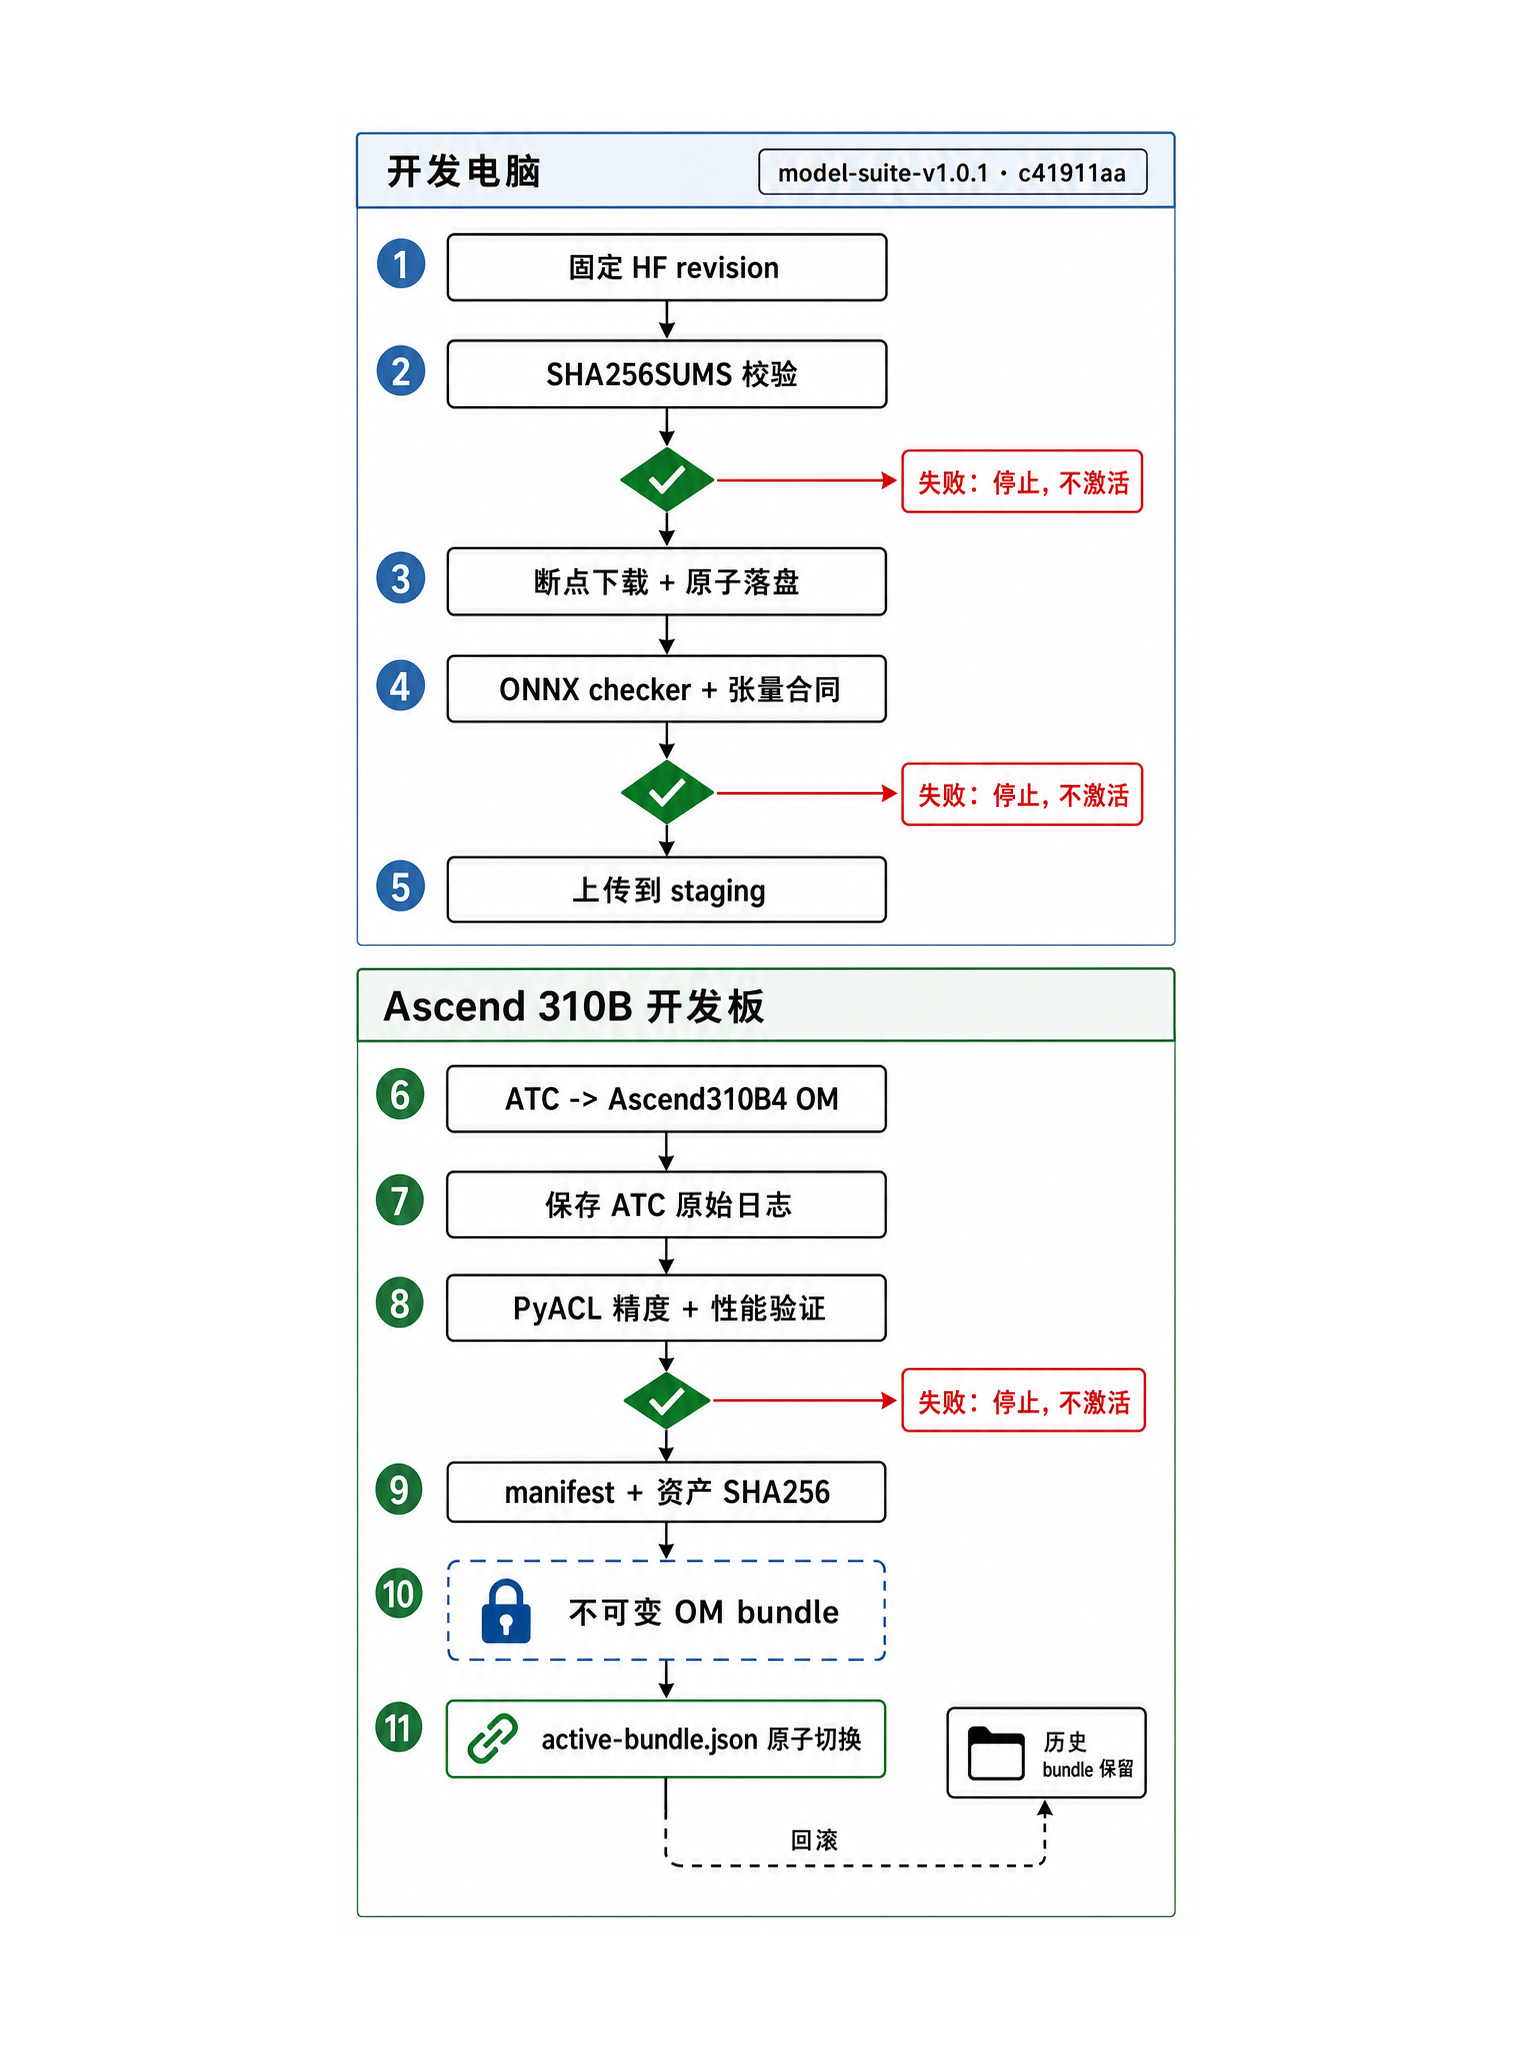
\includegraphics[keepaspectratio,alt={固定模型发布从下载校验、板端 ATC、PyACL 验证到不可变 bundle 原子激活的流程}]{cases/img3/case3-model-deployment-pipeline.png}}
\caption{固定模型发布从下载校验、板端 ATC、PyACL 验证到不可变 bundle
原子激活的流程}
\end{figure}

开发板使用现有 CANN 环境执行 ATC，目标 SoC 为
\passthrough{\lstinline!Ascend310B4!}；参数含义和版本要求应以
\href{https://www.hiascend.com/document}{Ascend CANN 官方文档}为准。ONNX
文件先按 \href{https://onnx.ai/onnx/}{ONNX 官方规范和
checker}检查。Piano-DDSP 当前使用
\passthrough{\lstinline!precision\_mode\_v2=origin!} 的 FP32 GRU
展开图；DDSP-VST Feature 选择
\passthrough{\lstinline!mixed\_float16!}，因为它通过了
\passthrough{\lstinline!1,000!} 帧精度和 Feature+Control
\passthrough{\lstinline!p95 < 20 ms!} 验证，而
\passthrough{\lstinline!force\_fp16!} 候选被精度门槛拒绝。

一个可进入运行目录的 bundle 至少应包含：

{ % do not increment counter
\begin{longtable}[]{@{}ll@{}}
\toprule\noalign{}
证据 & 目的 \\
\midrule\noalign{}
\endhead
\bottomrule\noalign{}
\endlastfoot
源 ONNX SHA256 与固定 revision & 证明转换输入没有漂移 \\
OM SHA256 与目标 SoC & 证明运行文件和硬件目标一致 \\
原始 ATC 日志与摘要 & 保留编译参数、退出码和算子诊断 \\
输入输出张量合同 & 阻止名称、形状和类型错配 \\
参考 NPZ 与误差报告 & 比较 ONNX/TFLite 参考和 OM 输出 \\
性能报告 & 记录 warmup、循环次数、p50、p95、p99 \\
manifest 与许可证 & 让服务端只发现完整、可追溯资产 \\
\end{longtable}
}

\subsection{生产运行时严格 OM-only}\label{src-experiment-case3-om-only}

生产服务只接受目录中的模型
ID，不接受浏览器提交任意文件路径或后端名称。Piano、MIDI-DDSP、DDSP-VST
Feature 和 Control 的实际后端都必须报告为
\passthrough{\lstinline!acl/om!}。模型缺失、哈希不符、张量不符、NPU
不可用或实体 capture 消失时，服务拒绝启动并释放资源；不会切换到 ONNX
Runtime、TFLite、浏览器推理或 CPU 神经网络。

\section{7. 后端设计}\label{src-experiment-case3-backend}

\subsection{FastAPI、作业和文件资产}\label{src-experiment-case3-fastapi}

后端入口是
\href{https://github.com/zhouxzh/Ascend310/blob/main/samples/case3/midi_ddsp_webui/app.py}{\passthrough{\lstinline!midi\_ddsp\_webui/app.py!}}，由
\href{https://github.com/zhouxzh/Ascend310/blob/main/samples/case3/scripts/run_webui.py}{\passthrough{\lstinline!scripts/run\_webui.py!}}
在 \passthrough{\lstinline!0.0.0.0:8765!} 启动。FastAPI
同时提供生产静态资源、REST API、WebSocket、MIDI 上传、WAV
产物和状态页面。

\begin{figure}
\centering
\pandocbounded{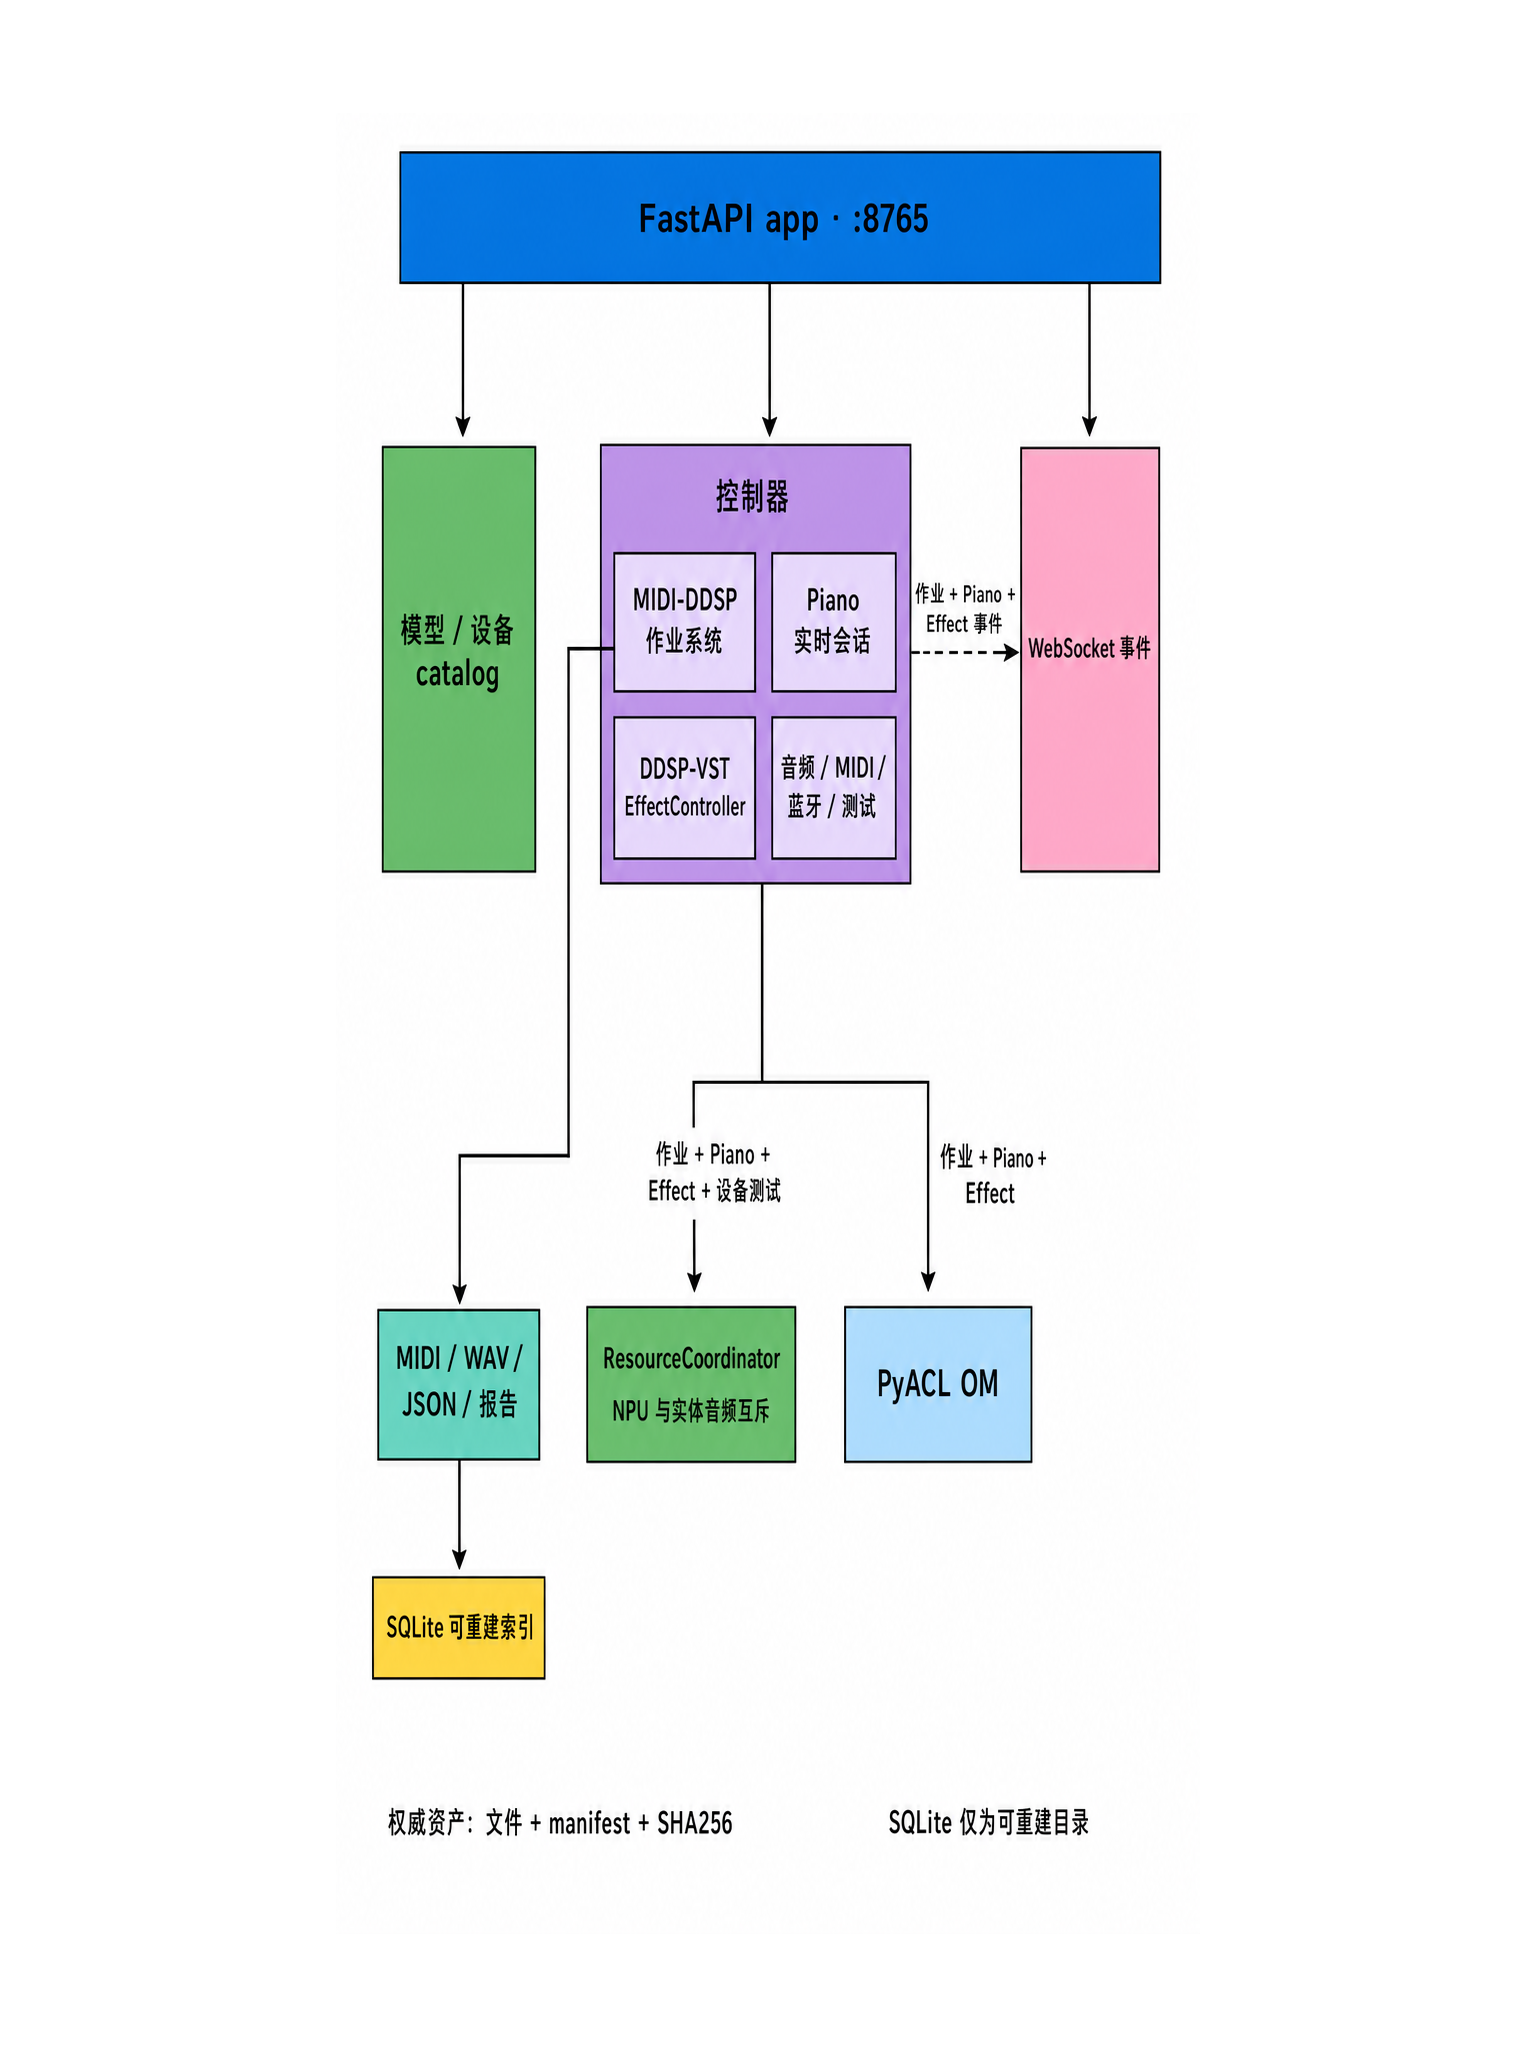
\includegraphics[keepaspectratio,alt={Case 3 FastAPI 后端的控制器、资源互斥、PyACL、事件和存储模块边界}]{cases/img3/case3-backend-architecture.png}}
\caption{Case 3 FastAPI
后端的控制器、资源互斥、PyACL、事件和存储模块边界}
\end{figure}

MIDI-DDSP 音频库使用 Python 标准库
\passthrough{\lstinline!sqlite3!}，数据库路径为
\passthrough{\lstinline!reports/webui/library.sqlite3!}。\passthrough{\lstinline!midi\_sources!}
以 MIDI 内容 SHA256 标识曲目，\passthrough{\lstinline!render\_versions!}
保存每次渲染的模型、声部分配、seed、增益、尾音、WAV
和报告引用；即使配置相同，显式渲染也会产生新历史。SQLite
只是可重建目录，真正权威的数据仍是
MIDI、WAV、任务元数据、manifest、报告和哈希文件。

\subsection{资源互斥与实时钢琴}\label{src-experiment-case3-resource-coordinator}

\passthrough{\lstinline!ResourceCoordinator!} 互斥以下会占用 NPU
或真实音频设备的流程：

\begin{itemize}
\tightlist
\item
  Piano-DDSP 触控与实体 MIDI 共享实时会话；
\item
  DDSP-VST Effect 双工链路；
\item
  MIDI-DDSP 板端 WAV 播放；
\item
  麦克风输入测试；
\item
  扬声器左右声道测试。
\end{itemize}

发生冲突时 API 返回
\passthrough{\lstinline!409!}，而不是同时打开设备。停止、异常、设备断开和线程退出都必须释放锁。浏览器不能绕过协调器直接选择板端文件路径。

Piano worker 是独立常驻子进程。MIDI 的
\passthrough{\lstinline!note\_on!} 立即进入状态机，早到的
\passthrough{\lstinline!note\_off!} 只在合成状态内部延迟，保证至少四个
\passthrough{\lstinline!4 ms!} 帧，即 \passthrough{\lstinline!16 ms!}
的可听门长。这样既保留触摸响应，也避免一次浏览器帧内的快速按下和释放被合成为零长度声音。重复音符、CC64
延音、voice stealing、\passthrough{\lstinline!panic!} 和
\passthrough{\lstinline!release\_source!} 必须共同维护 16
个声部槽位，不能留下悬挂音符或踏板。

合成结果先进入有界 FIFO，再按 low、balanced 或 safe
延迟档合并音频块，通过所选的 PulseAudio、PortAudio 或板载
\passthrough{\lstinline!alsa\_mono!}
后端写入明确设备。输出增益是合成内部的
\passthrough{\lstinline!-60..+6 dB!}，默认
\passthrough{\lstinline!0 dB!}；它不会修改
PulseAudio、ALSA、浏览器或音箱硬件音量。

\subsection{DDSP-VST
音频线程与安全控制}\label{src-experiment-case3-effect-runtime}

Effect
的固定链路为：\passthrough{\lstinline!48 kHz 双声道摄像头输入 -> 单声道 -> 16 kHz -> 1024 窗/320 步长 -> Feature OM -> Control OM -> DDSP 合成 -> 48 kHz 双声道输出!}。输入和输出使用
\passthrough{\lstinline!parec!}、\passthrough{\lstinline!paplay!} 对应的
PulseAudio source/sink，不使用 monitor，也不在设备丢失后自动改路。

噪声门先校准环境底噪，再用开启阈值、迟滞、保持、开启和关闭时间平滑门增益。默认只输出转换后的声音，输出增益为
\passthrough{\lstinline!-18 dB!}。持续过载会进入明确的安全静音，并在状态和
WebSocket 中报告；不会继续输出可能削波的声音。

\begin{figure}
\centering
\pandocbounded{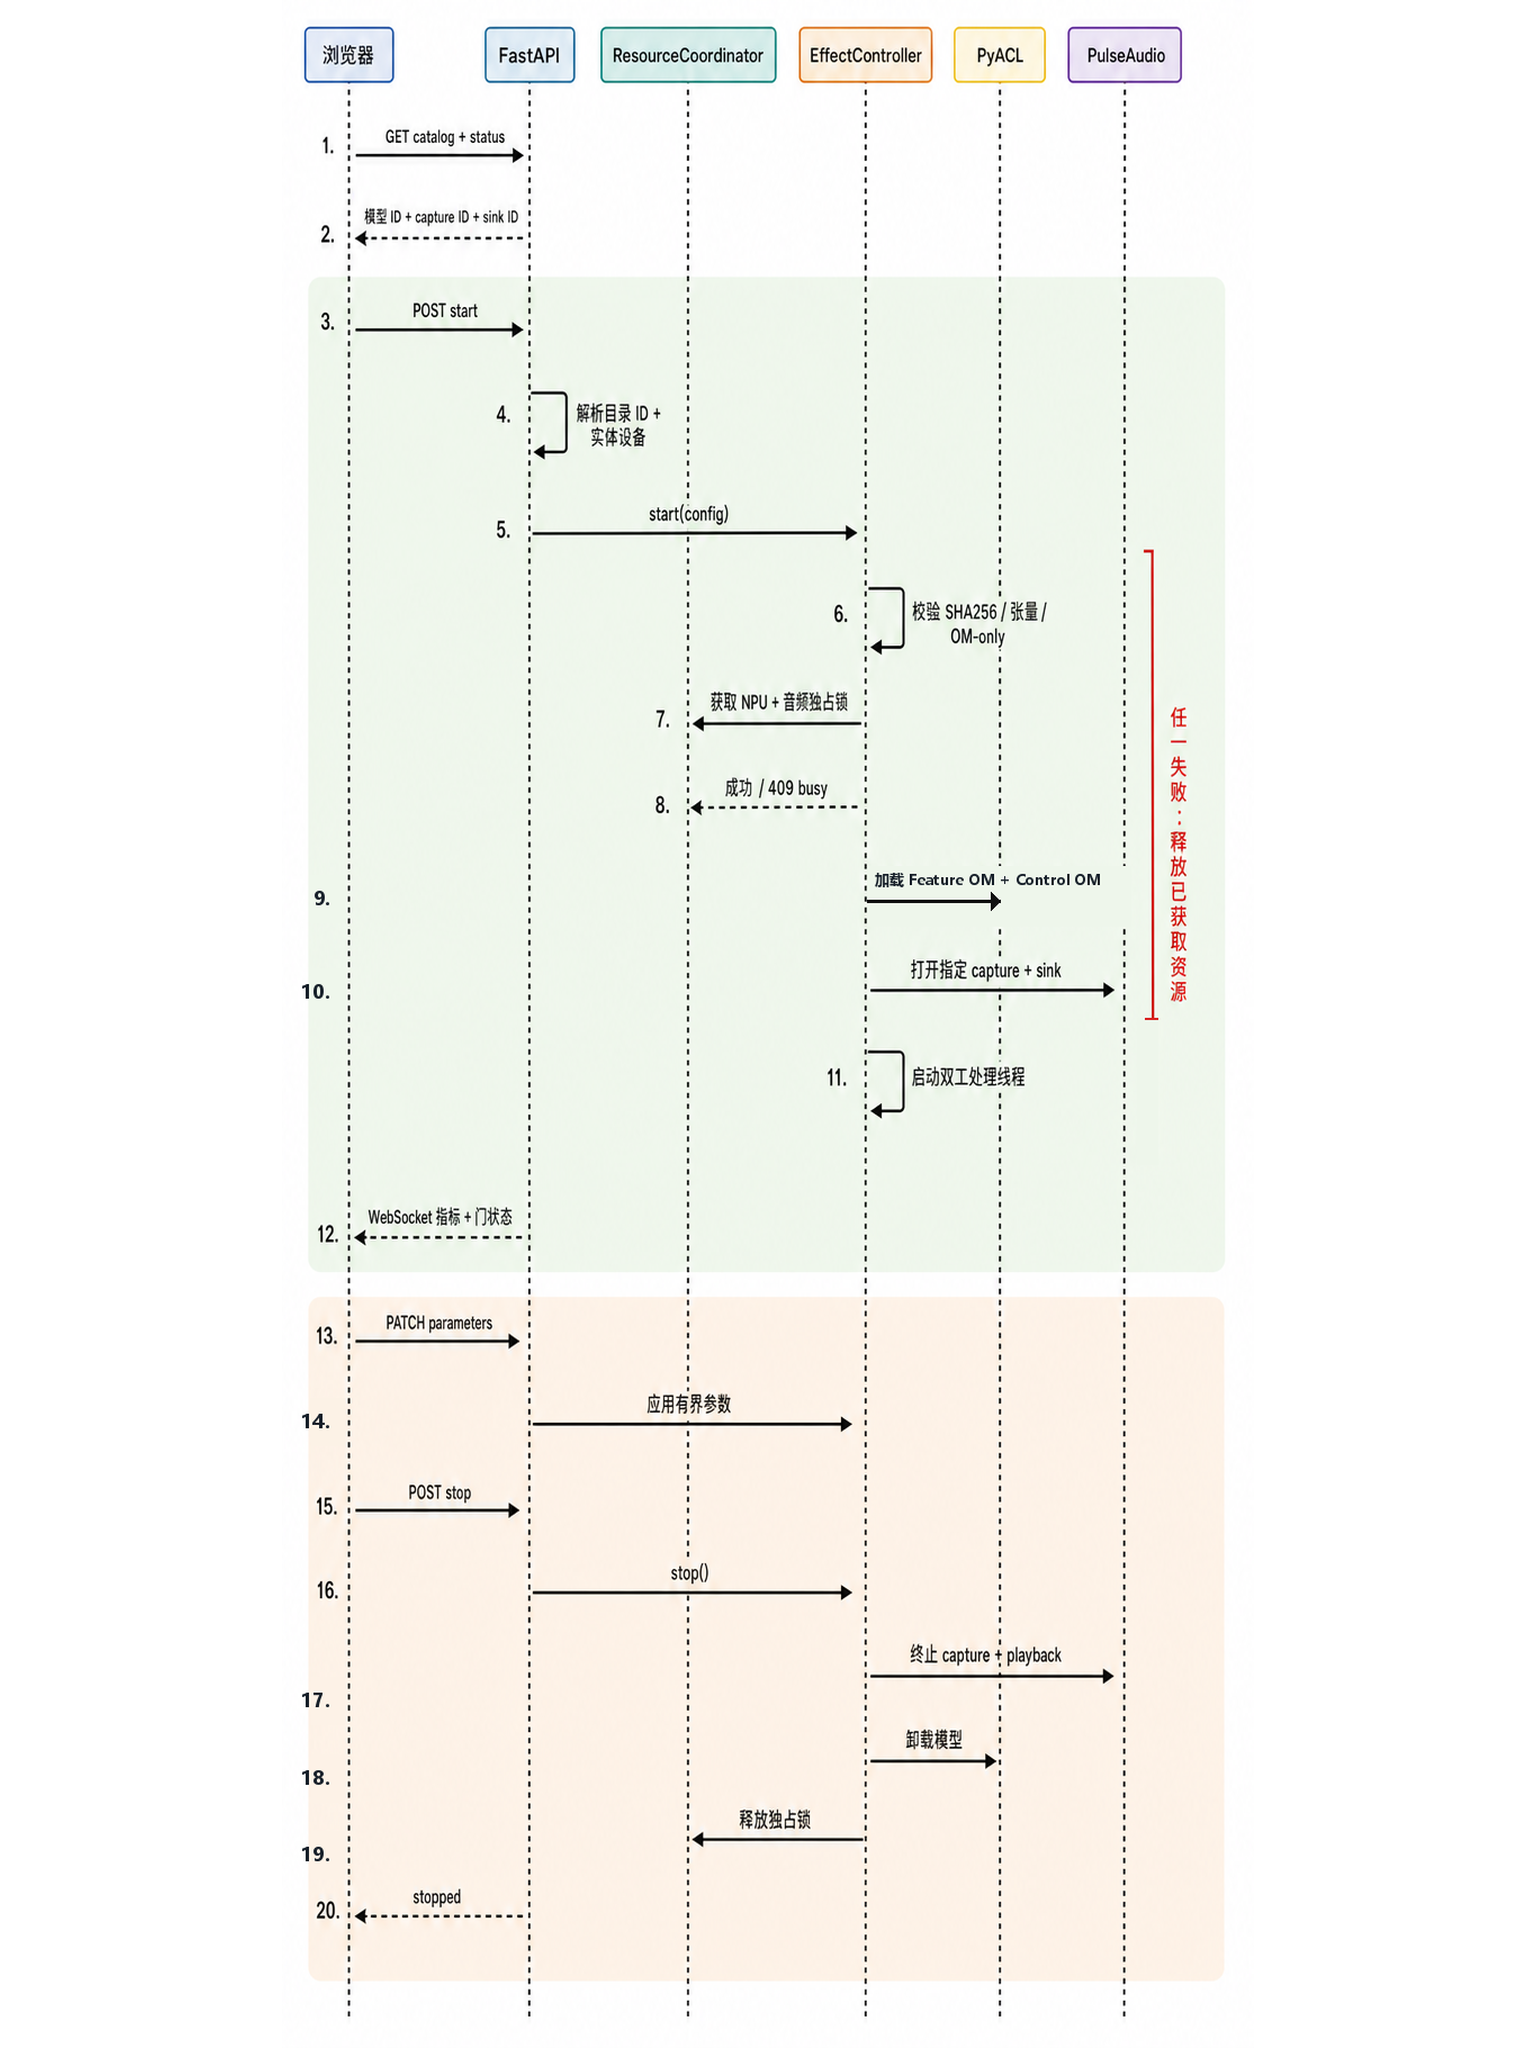
\includegraphics[keepaspectratio,alt={DDSP-VST Effect 从目录查询、资源加锁和模型启动到有序停止释放的时序}]{cases/img3/case3-ddsp-vst-sequence.png}}
\caption{DDSP-VST Effect
从目录查询、资源加锁和模型启动到有序停止释放的时序}
\end{figure}

\subsection{主要 API}\label{src-experiment-case3-api}

{ % do not increment counter
\begin{longtable}[]{@{}
  >{\raggedright\arraybackslash}p{(\linewidth - 4\tabcolsep) * \real{0.3333}}
  >{\raggedright\arraybackslash}p{(\linewidth - 4\tabcolsep) * \real{0.3333}}
  >{\raggedright\arraybackslash}p{(\linewidth - 4\tabcolsep) * \real{0.3333}}@{}}
\toprule\noalign{}
\begin{minipage}[b]{\linewidth}\raggedright
类别
\end{minipage} & \begin{minipage}[b]{\linewidth}\raggedright
代表接口
\end{minipage} & \begin{minipage}[b]{\linewidth}\raggedright
作用
\end{minipage} \\
\midrule\noalign{}
\endhead
\bottomrule\noalign{}
\endlastfoot
系统 &
\passthrough{\lstinline!GET /api/v1/status!}、\passthrough{\lstinline!GET /api/v1/catalog!}
& 主机、依赖、NPU、模型和作业摘要 \\
实时钢琴 & \passthrough{\lstinline!GET /api/v1/realtime/catalog|status!}
& 查询 patch、输出、MIDI 和会话状态 \\
实时钢琴 &
\passthrough{\lstinline!POST /api/v1/realtime/start|switch|stop|panic!}
& 启动、切换、停止和紧急释放共享会话 \\
实时钢琴 & \passthrough{\lstinline!PATCH /api/v1/realtime/parameters!} &
实时更新增益、移调、混响等有界参数 \\
MIDI-DDSP &
\passthrough{\lstinline!POST /api/v1/midi-files!}、\passthrough{\lstinline!POST /api/v1/midi-ddsp/jobs!}
& 上传 MIDI，创建渲染任务 \\
音频库 & \passthrough{\lstinline!GET /api/v1/midi-ddsp/library!} &
曲目、版本、首选版本和可用性 \\
MIDI 解析 &
\passthrough{\lstinline!GET /api/v1/midi-files/\{midi\_id\}/voices|piano-roll!}
& 声部分离结果与浏览器钢琴卷帘数据 \\
DDSP-VST &
\passthrough{\lstinline!GET /api/v1/ddsp-vst-effect/catalog|status!} &
OM-only 模型与实体设备目录 \\
DDSP-VST &
\passthrough{\lstinline!POST /api/v1/ddsp-vst-effect/start|stop|calibrate!}
& Effect 生命周期和底噪校准 \\
DDSP-VST &
\passthrough{\lstinline!PATCH /api/v1/ddsp-vst-effect/parameters!} &
更新音色、门限、谐波、噪声、增益和混响 \\
设备 &
\passthrough{\lstinline!GET /api/v1/speaker-outputs!}、\passthrough{\lstinline!GET /api/v1/audio-inputs!}、\passthrough{\lstinline!GET /api/v1/midi-ddsp/audio-devices!}、\passthrough{\lstinline!GET /api/v1/midi-ports!}
& 显式枚举各工作流的输入输出和 MIDI \\
测试 & 扬声器、输入测试和蓝牙接口 & 独占测试与设备管理 \\
WebSocket &
\passthrough{\lstinline!/api/v1/events!}、\passthrough{\lstinline!/api/v1/realtime/events!}
& 作业状态，以及音符、踏板、弯音、录音、监听和运行指标 \\
WebSocket & \passthrough{\lstinline!/api/v1/ddsp-vst-effect/events!} &
音高、响度、延迟、门与安全静音 \\
\end{longtable}
}

详细字段、状态和同源限制见\href{https://github.com/zhouxzh/Ascend310/blob/main/samples/case3/doc/webui.md}{WebUI
与 API 指南}。服务没有身份认证，只适合可信局域网。

\section{8. 前端设计}\label{src-experiment-case3-frontend}

\subsection{技术栈与应用壳}\label{src-experiment-case3-frontend-stack}

前端使用 React 19、TypeScript、Vite、Lucide 图标、Canvas、Vitest 和
Playwright。\href{https://github.com/zhouxzh/Ascend310/blob/main/samples/case3/webui/src/App.tsx}{\passthrough{\lstinline!webui/src/App.tsx!}}
提供固定四项顶层导航：实时演奏、MIDI-DDSP、DDSP-VST
和设备；实时演奏内部使用分段控件切换触摸屏与 MIDI
键盘输入模式。四个工作区使用懒加载，首次进入时显示稳定加载状态；DDSP-VST
首次打开后保留挂载，隐藏时停止 Canvas
绘制，避免重复初始化实时资源。应用每 \passthrough{\lstinline!5 s!}
刷新低频系统状态，同时由 WebSocket 推送作业、音频设备、实时演奏事件和
Effect 指标。

前端只提交服务端目录提供的模型 ID、设备 ID
和有边界参数。错误、不可用、运行、暂停、门关闭、安全静音和 Health Alarm
都同时使用文字与颜色表达，不能只靠颜色区分。

\passthrough{\lstinline!RealtimePerformanceView!}
把当前钢琴音色、音频输出、MIDI 端口、延时档、各音色参数，以及触摸屏和
MIDI
键盘各自的键数、起始音和触控键盘大小保存在版本化浏览器配置中。恢复配置时仍以服务端目录和参数边界为准；会话运行、录音或切换期间锁定输入方式和设备选择，浏览器本地状态不能替代后端会话状态。

\subsection{两个钢琴卷帘的时间模型}\label{src-experiment-case3-canvas}

\passthrough{\lstinline!LivePianoRoll!} 与
\passthrough{\lstinline!MidiFilePianoRoll!} 都使用 Canvas，但不能合并：

{ % do not increment counter
\begin{longtable}[]{@{}
  >{\raggedright\arraybackslash}p{(\linewidth - 6\tabcolsep) * \real{0.2500}}
  >{\raggedright\arraybackslash}p{(\linewidth - 6\tabcolsep) * \real{0.2500}}
  >{\raggedright\arraybackslash}p{(\linewidth - 6\tabcolsep) * \real{0.2500}}
  >{\raggedright\arraybackslash}p{(\linewidth - 6\tabcolsep) * \real{0.2500}}@{}}
\toprule\noalign{}
\begin{minipage}[b]{\linewidth}\raggedright
组件
\end{minipage} & \begin{minipage}[b]{\linewidth}\raggedright
时间来源
\end{minipage} & \begin{minipage}[b]{\linewidth}\raggedright
绘制策略
\end{minipage} & \begin{minipage}[b]{\linewidth}\raggedright
性能边界
\end{minipage} \\
\midrule\noalign{}
\endhead
\bottomrule\noalign{}
\endlastfoot
\passthrough{\lstinline!LivePianoRoll!} & WebSocket 的实时 note edge &
静态键位/网格缓存，动态轨迹单层更新 & 最多 30 FPS，像素比上限
1.25，历史最多 192 条，空闲时停止 \\
\passthrough{\lstinline!MidiFilePianoRoll!} & 完整 MIDI 时间轴与播放位置
& 静态网格、音符层、动态光标三层 Canvas & 可显示 10,000
音符，不创建逐音符 React/SVG 节点，空闲时停止动画 \\
\end{longtable}
}

实时卷帘保留短音符的最小可见高度；状态快照只用于重新同步当前按键，不能反推已错过的短音符。文件卷帘支持声部颜色、拍号网格、缩放、拖动、进度光标和活动音符，但不是
MIDI 编辑器。

\subsection{触摸屏、桌面和手机布局}\label{src-experiment-case3-responsive}

10 英寸板端物理屏幕为 \passthrough{\lstinline!1920 x 1080!}，Firefox
kiosk 的浏览器内容视口约为
\passthrough{\lstinline!1920 x 969!}。主要导航使用
\passthrough{\lstinline!20-22 px!} 字体，正文和控件以
\passthrough{\lstinline!16 px!} 为目标，次要文字不小于
\passthrough{\lstinline!14 px!}；主要操作高度至少
\passthrough{\lstinline!56 px!}，普通触控目标至少
\passthrough{\lstinline!52 px!}。页面不能依赖浏览器只报告 coarse
pointer，因此还使用板端尺寸和页面类触发触摸布局。

窄手机隐藏完整顶部导航并使用带安全区的底部导航。所有支持视口都要求无文档级横向滚动、无控件重叠、文本不被截断，并保留
\passthrough{\lstinline!tablist!}、\passthrough{\lstinline!tab!}、\passthrough{\lstinline!tabpanel!}、键盘焦点和可访问名称。

\section{9. 逐页界面与操作说明}\label{src-experiment-case3-ui-guide}

本节 12 张截图均在 2026-08-04 从真实
\passthrough{\lstinline!ascend8t:8765!} 生产服务的 Firefox kiosk
重新采集，物理屏幕分辨率为
\passthrough{\lstinline!1920 x 1080!}，没有使用模拟 API。界面上的
\passthrough{\lstinline!NPU ALARM!} 是该板
\passthrough{\lstinline!npu-smi!} 的真实警告；只要 NPU 可见且真实 OM
推理通过，它不自动等同于推理失败。

\subsection{实时演奏 / 触摸屏}\label{src-experiment-case3-ui-touch}

\begin{figure}
\centering
\pandocbounded{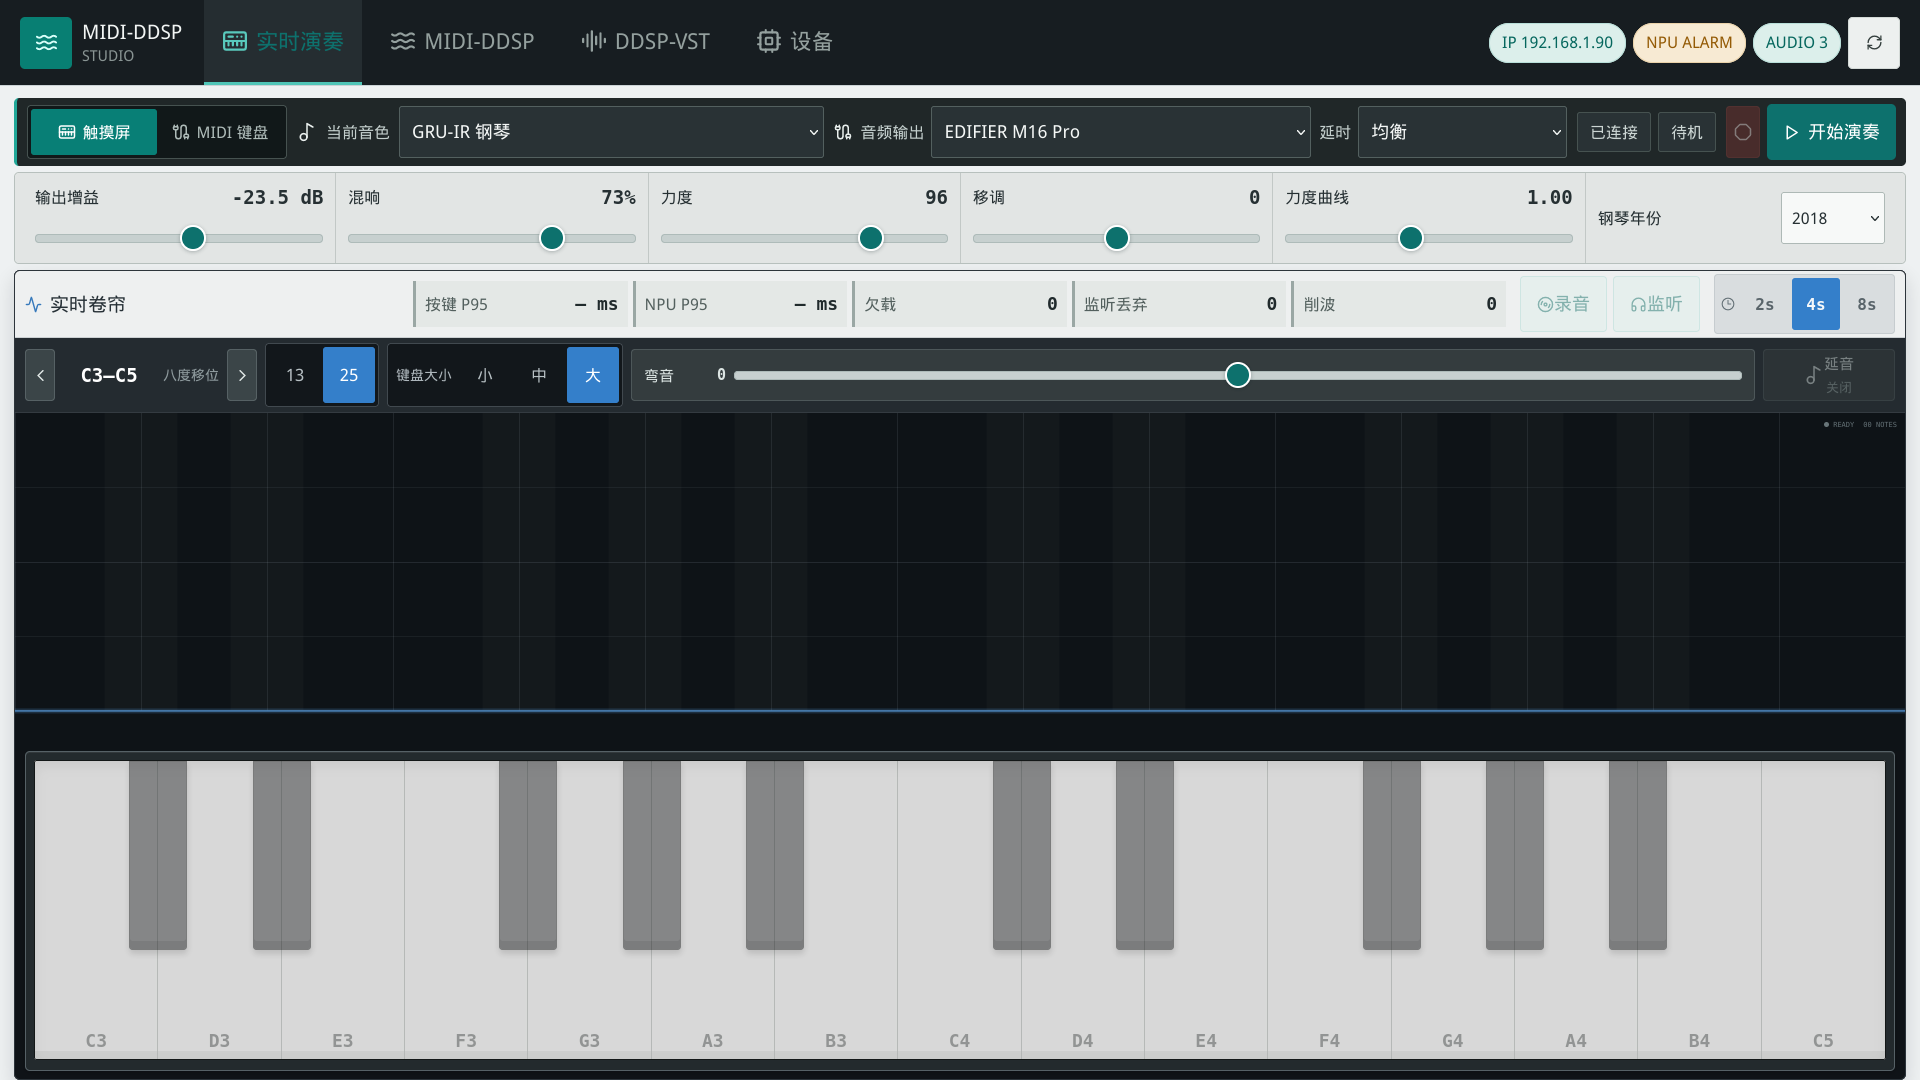
\includegraphics[keepaspectratio,alt={实时演奏工作区的触摸屏模式}]{cases/img3/case3-ui-touch-performance.png}}
\caption{实时演奏工作区的触摸屏模式}
\end{figure}

{ % do not increment counter
\begin{longtable}[]{@{}
  >{\raggedright\arraybackslash}p{(\linewidth - 8\tabcolsep) * \real{0.2000}}
  >{\raggedright\arraybackslash}p{(\linewidth - 8\tabcolsep) * \real{0.2000}}
  >{\raggedright\arraybackslash}p{(\linewidth - 8\tabcolsep) * \real{0.2000}}
  >{\raggedright\arraybackslash}p{(\linewidth - 8\tabcolsep) * \real{0.2000}}
  >{\raggedright\arraybackslash}p{(\linewidth - 8\tabcolsep) * \real{0.2000}}@{}}
\toprule\noalign{}
\begin{minipage}[b]{\linewidth}\raggedright
区域
\end{minipage} & \begin{minipage}[b]{\linewidth}\raggedright
控件
\end{minipage} & \begin{minipage}[b]{\linewidth}\raggedright
作用
\end{minipage} & \begin{minipage}[b]{\linewidth}\raggedright
正常状态
\end{minipage} & \begin{minipage}[b]{\linewidth}\raggedright
注意事项
\end{minipage} \\
\midrule\noalign{}
\endhead
\bottomrule\noalign{}
\endlastfoot
统一会话栏 & 输入方式、当前音色、音频输出、延时档、开始/停止、Panic &
管理共享 Piano-DDSP 会话 & 截图为已连接、待机 &
会话运行、录音或切换时不能更换输入方式；Panic 用于释放悬挂音符 \\
参数带 & 输出增益、混响、触控力度、移调、力度曲线、钢琴年份 &
实时改变当前钢琴音色参数 & 数值稳定，不改变布局 &
输出增益不是系统音量，参数值受服务端目录约束 \\
卷帘工具栏 & 按键 P95、NPU P95、欠载、监听丢弃、削波、录音、监听、2/4/8
秒 & 查看会话指标和实时 note edge & 待机指标为空或为 0，运行后更新 &
短音符保留最小可见轨迹，监听和录音只在会话运行时可用 \\
触控命令栏 & 13/25 键、小/中/大、八度、弯音、延音 &
调整屏幕琴键范围并演奏 & 截图为 25 键与大键盘 &
无缓存时键盘大小默认为``中''；弯音松开自动回中，88 键只属于 MIDI
键盘模式 \\
底部钢琴 & 触控白键和黑键 & 手指直接发送
\passthrough{\lstinline!note\_on!}/\passthrough{\lstinline!note\_off!} &
待机可查看音域，开始后发声 & 快速松开仍由后端保证 16 ms
门长；失焦、取消触摸或停止会全部停音 \\
\end{longtable}
}

\subsection{实时演奏 / MIDI
键盘}\label{src-experiment-case3-ui-midi-keyboard}

\begin{figure}
\centering
\pandocbounded{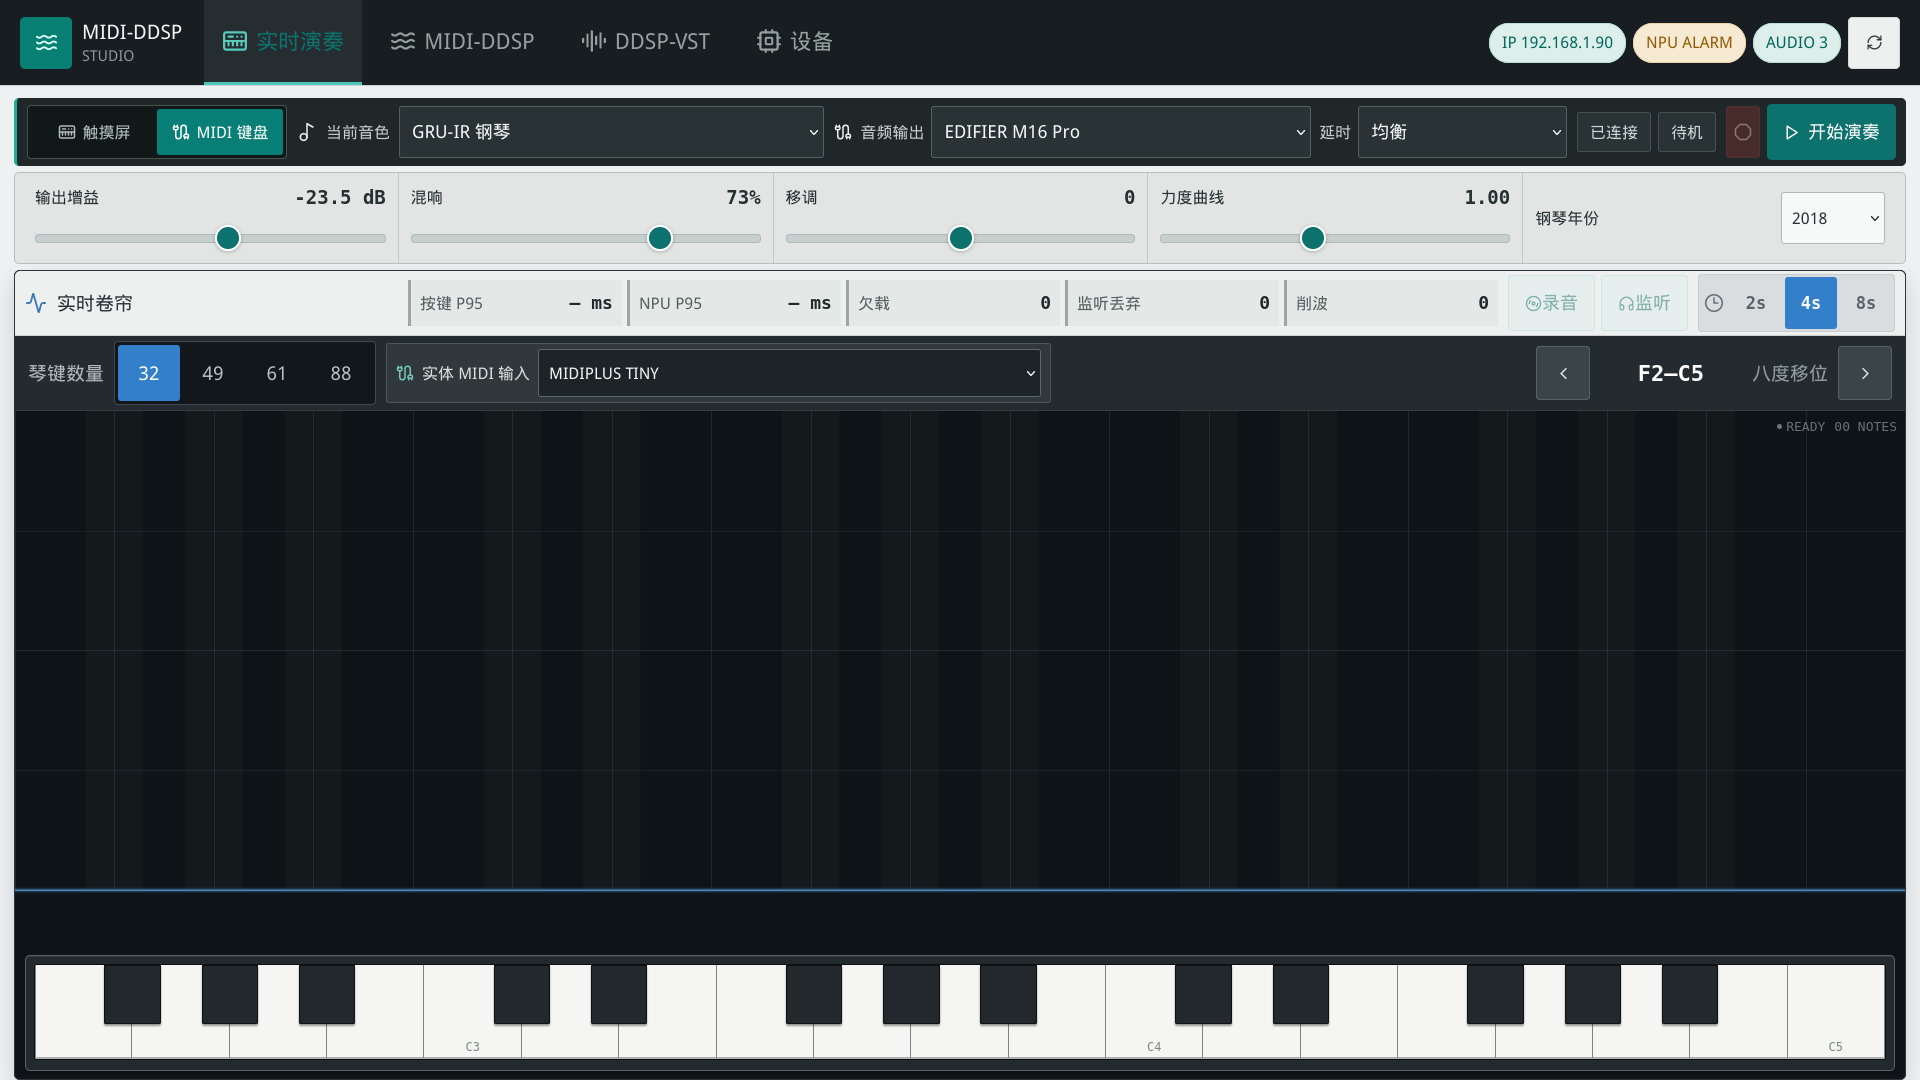
\includegraphics[keepaspectratio,alt={实时演奏工作区的 MIDI 键盘模式}]{cases/img3/case3-ui-midi-keyboard.png}}
\caption{实时演奏工作区的 MIDI 键盘模式}
\end{figure}

{ % do not increment counter
\begin{longtable}[]{@{}
  >{\raggedright\arraybackslash}p{(\linewidth - 8\tabcolsep) * \real{0.2000}}
  >{\raggedright\arraybackslash}p{(\linewidth - 8\tabcolsep) * \real{0.2000}}
  >{\raggedright\arraybackslash}p{(\linewidth - 8\tabcolsep) * \real{0.2000}}
  >{\raggedright\arraybackslash}p{(\linewidth - 8\tabcolsep) * \real{0.2000}}
  >{\raggedright\arraybackslash}p{(\linewidth - 8\tabcolsep) * \real{0.2000}}@{}}
\toprule\noalign{}
\begin{minipage}[b]{\linewidth}\raggedright
区域
\end{minipage} & \begin{minipage}[b]{\linewidth}\raggedright
控件
\end{minipage} & \begin{minipage}[b]{\linewidth}\raggedright
作用
\end{minipage} & \begin{minipage}[b]{\linewidth}\raggedright
正常状态
\end{minipage} & \begin{minipage}[b]{\linewidth}\raggedright
注意事项
\end{minipage} \\
\midrule\noalign{}
\endhead
\bottomrule\noalign{}
\endlastfoot
统一会话栏与参数带 &
当前钢琴音色、音频输出、延时档、输出增益、混响、移调和力度曲线 &
与触摸屏模式共享 Piano-DDSP 会话 & 截图为已连接、待机 &
本页没有第二套音色参数，也不加载 DDSP-VST Synth 或 MIDI 文件抽屉 \\
键盘范围 & 32/49/61/88 键、八度 & 匹配实体控制器与可视范围 & MIDIPLUS
TINY 显示 32 键 & 小于 88 键可逐八度移动；88 键固定为 A0-C8 \\
实体 MIDI 输入 & 服务端端口下拉框 & 绑定板端枚举的输入端口 & MIDIPLUS
TINY 被选中 & 浏览器 Web MIDI
不是输入来源；运行中不能换端口，断开时释放该来源音符 \\
卷帘工具栏 & 会话指标、录音、监听、2/4/8 秒 & 观察真实 WebSocket
音符边沿和运行状态 & 短音符仍有可见标记 &
不用轮询替代边沿事件；录音、监听和指标与触摸屏模式共享 \\
可视键盘 & 只读键位高亮 & 对照实体 MIDI 的当前音符和音域 & 32 键范围为
F2-C5 & 只用于反馈，不在此处提供鼠标或触控演奏 \\
\end{longtable}
}

\subsection{MIDI-DDSP 音频库}\label{src-experiment-case3-ui-library}

\begin{figure}
\centering
\pandocbounded{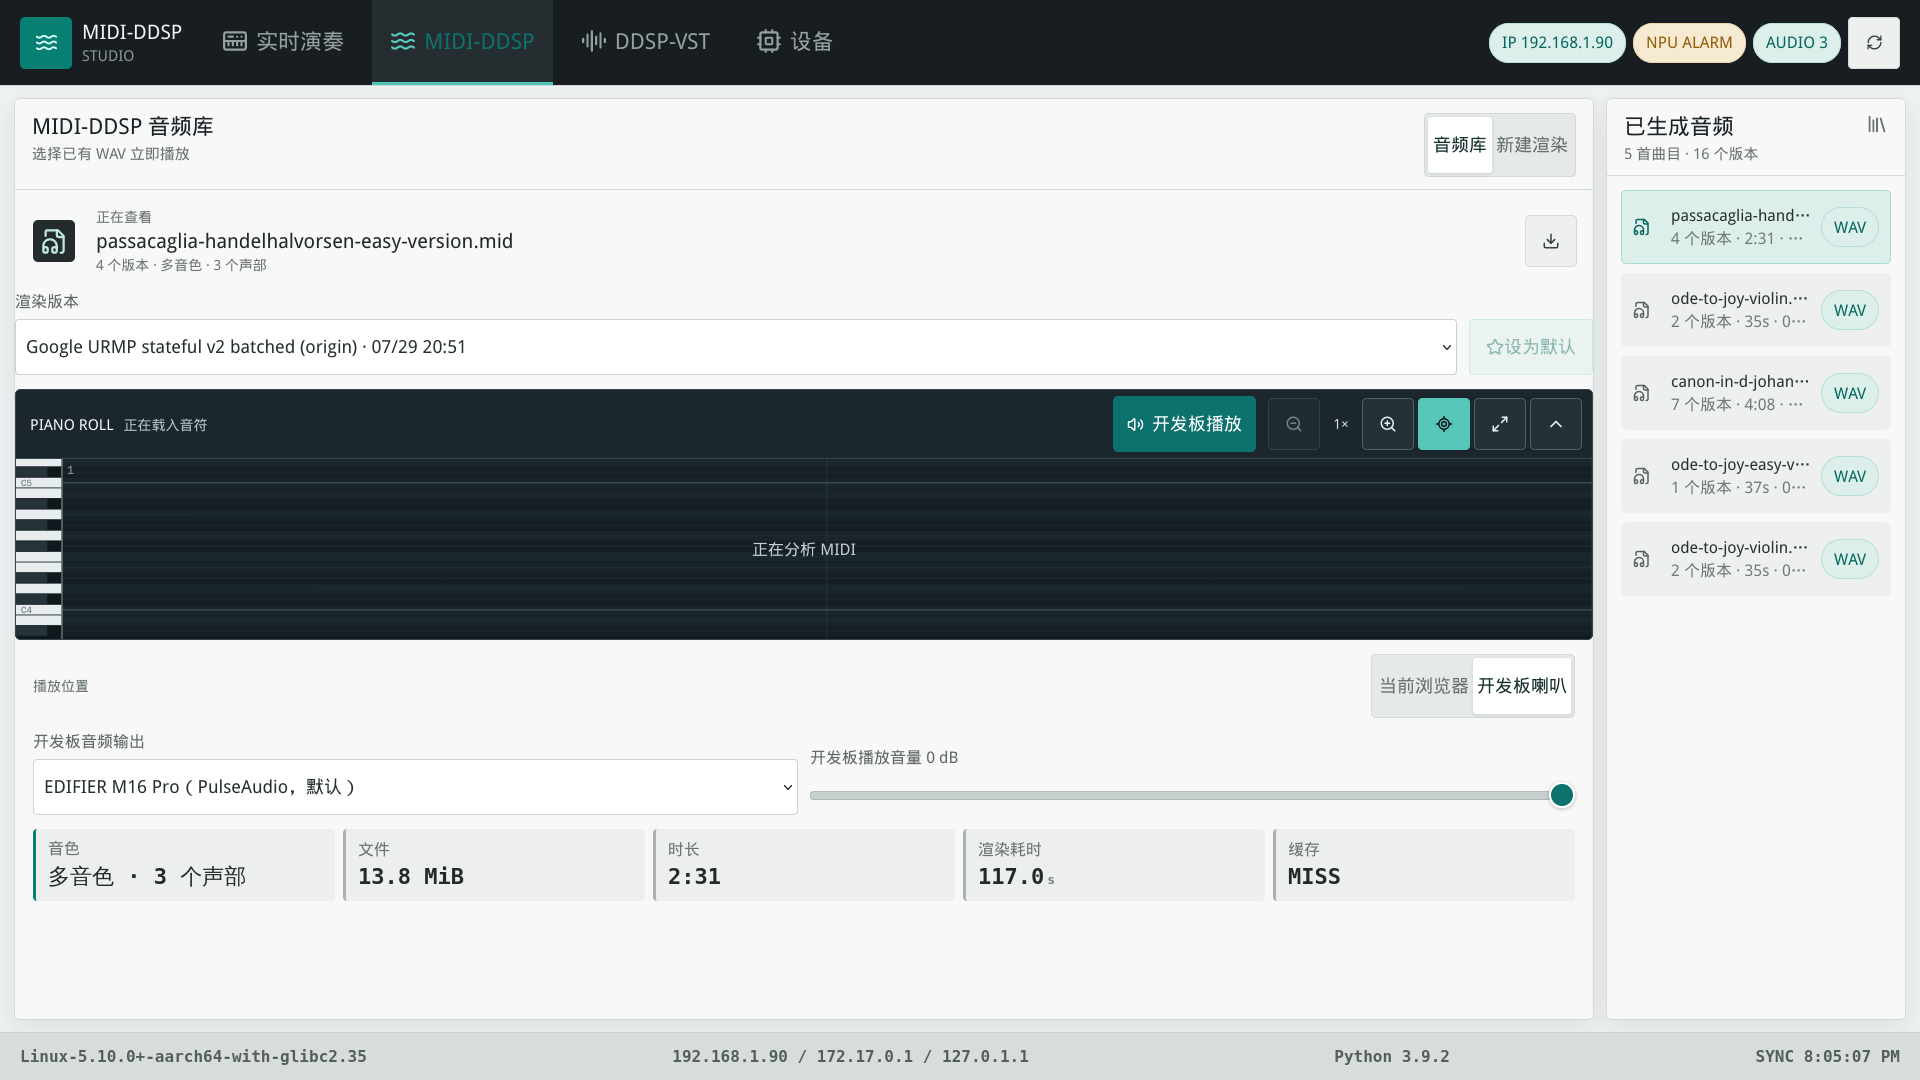
\includegraphics[keepaspectratio,alt={MIDI-DDSP 音频库页面}]{cases/img3/case3-ui-midi-ddsp-library.png}}
\caption{MIDI-DDSP 音频库页面}
\end{figure}

{ % do not increment counter
\begin{longtable}[]{@{}
  >{\raggedright\arraybackslash}p{(\linewidth - 8\tabcolsep) * \real{0.2000}}
  >{\raggedright\arraybackslash}p{(\linewidth - 8\tabcolsep) * \real{0.2000}}
  >{\raggedright\arraybackslash}p{(\linewidth - 8\tabcolsep) * \real{0.2000}}
  >{\raggedright\arraybackslash}p{(\linewidth - 8\tabcolsep) * \real{0.2000}}
  >{\raggedright\arraybackslash}p{(\linewidth - 8\tabcolsep) * \real{0.2000}}@{}}
\toprule\noalign{}
\begin{minipage}[b]{\linewidth}\raggedright
区域
\end{minipage} & \begin{minipage}[b]{\linewidth}\raggedright
控件
\end{minipage} & \begin{minipage}[b]{\linewidth}\raggedright
作用
\end{minipage} & \begin{minipage}[b]{\linewidth}\raggedright
正常状态
\end{minipage} & \begin{minipage}[b]{\linewidth}\raggedright
注意事项
\end{minipage} \\
\midrule\noalign{}
\endhead
\bottomrule\noalign{}
\endlastfoot
主标题 & 音频库/新建渲染 & 切换浏览与创建流程 & 音频库选中 &
两种流程不混在一个长页面 \\
曲目与版本 & 版本下拉、设为默认 & 一首 MIDI 管理多次渲染 & 版本、音色和
WAV 同步变化 & 缺失文件会标记不可用，不删除历史 \\
文件卷帘 & 缩放、跟随、全屏 & 查看完整 MIDI 和播放光标 & 仅一个可见卷帘
& 页面不恢复第二个波形动画 \\
播放区 & 开发板/浏览器、设备、增益 & 选择实际播放目标 & 默认开发板喇叭 &
浏览器播放不改变系统 mixer \\
右侧曲目列表 & 曲目、版本数、时长 & 快速切换音频库来源 &
选中项有文字和底色 & 选择不可用版本时返回错误 \\
\end{longtable}
}

\subsection{MIDI-DDSP 新建渲染}\label{src-experiment-case3-ui-render}

\begin{figure}
\centering
\pandocbounded{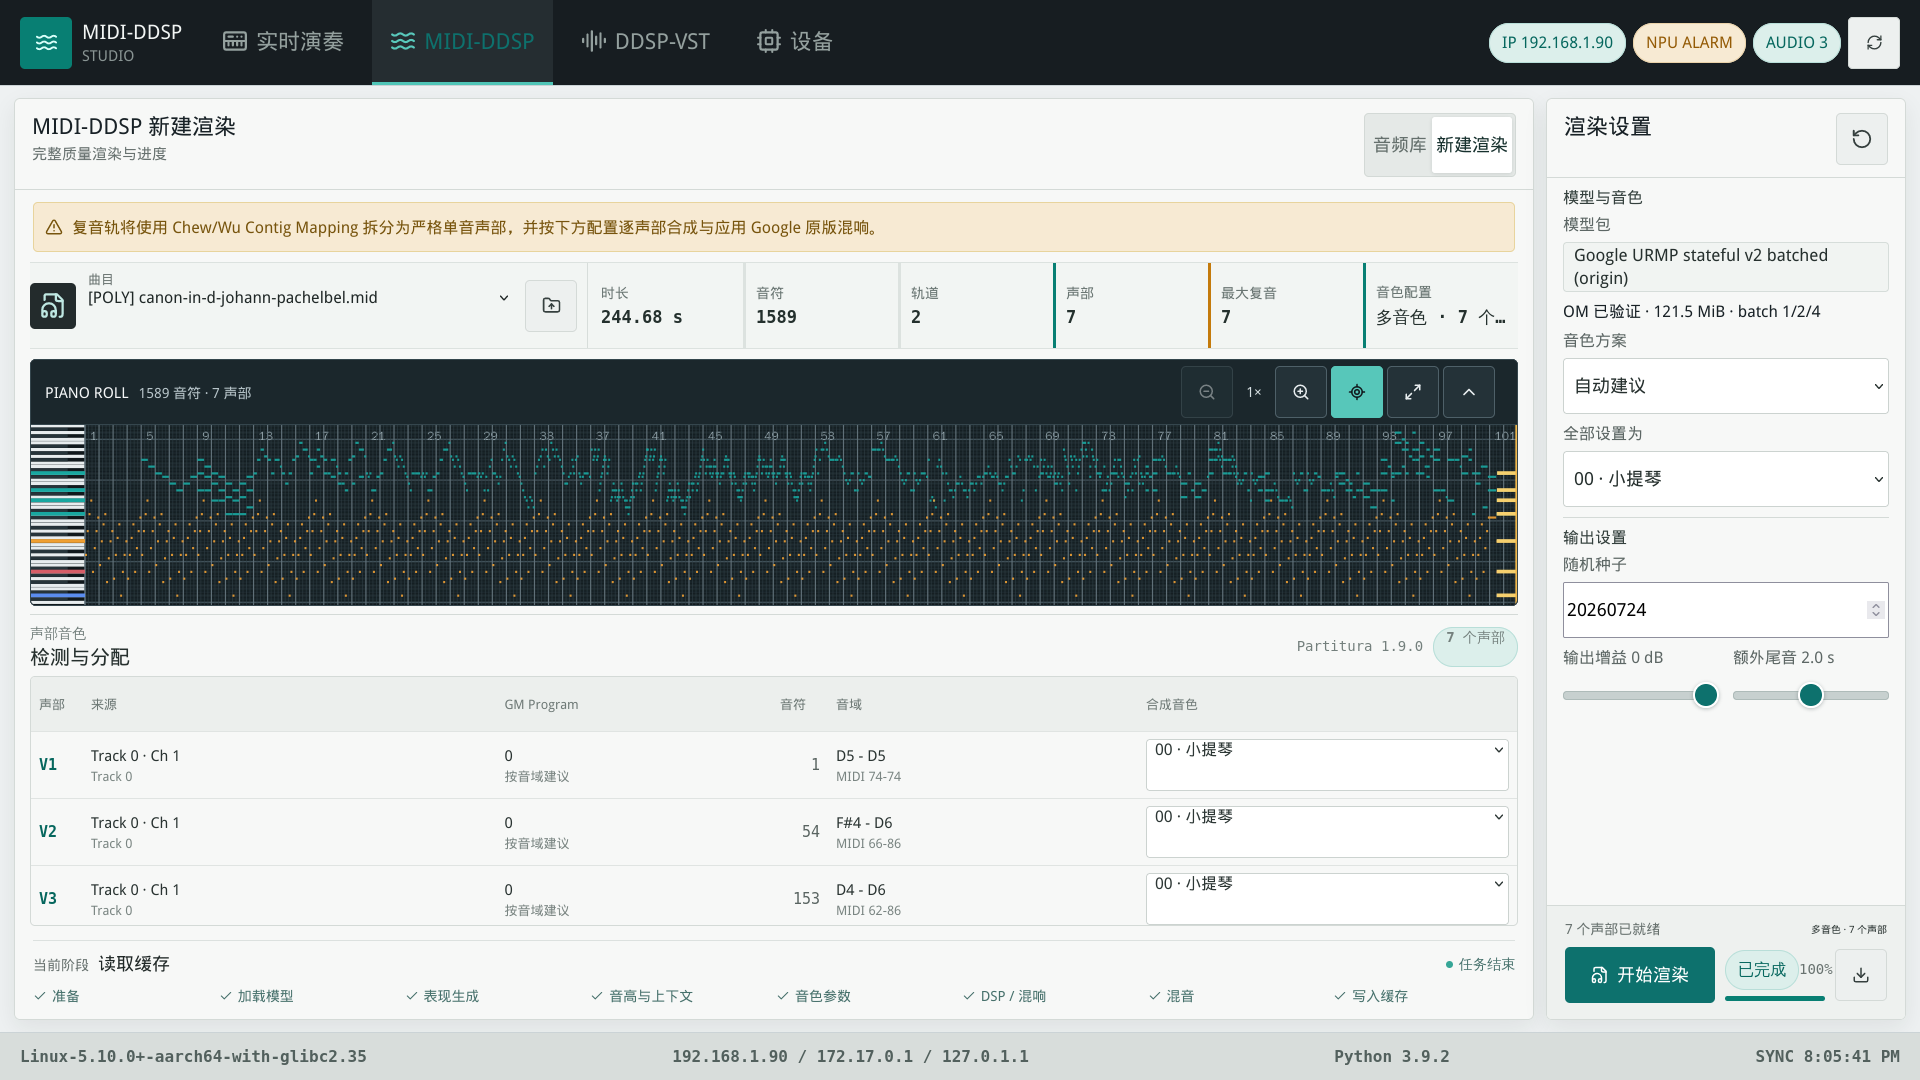
\includegraphics[keepaspectratio,alt={MIDI-DDSP 新建渲染页面}]{cases/img3/case3-ui-midi-ddsp-render.png}}
\caption{MIDI-DDSP 新建渲染页面}
\end{figure}

{ % do not increment counter
\begin{longtable}[]{@{}
  >{\raggedright\arraybackslash}p{(\linewidth - 8\tabcolsep) * \real{0.2000}}
  >{\raggedright\arraybackslash}p{(\linewidth - 8\tabcolsep) * \real{0.2000}}
  >{\raggedright\arraybackslash}p{(\linewidth - 8\tabcolsep) * \real{0.2000}}
  >{\raggedright\arraybackslash}p{(\linewidth - 8\tabcolsep) * \real{0.2000}}
  >{\raggedright\arraybackslash}p{(\linewidth - 8\tabcolsep) * \real{0.2000}}@{}}
\toprule\noalign{}
\begin{minipage}[b]{\linewidth}\raggedright
区域
\end{minipage} & \begin{minipage}[b]{\linewidth}\raggedright
控件
\end{minipage} & \begin{minipage}[b]{\linewidth}\raggedright
作用
\end{minipage} & \begin{minipage}[b]{\linewidth}\raggedright
正常状态
\end{minipage} & \begin{minipage}[b]{\linewidth}\raggedright
注意事项
\end{minipage} \\
\midrule\noalign{}
\endhead
\bottomrule\noalign{}
\endlastfoot
曲目栏 & MIDI 选择和上传 & 选择现有文件或上传受限格式 &
显示时长、音符、轨道和声部 & 只接受 \passthrough{\lstinline!.mid/.midi!}
和大小限制 \\
文件卷帘 & 声部颜色与视图控制 & 检查声部分离结果 & 声部数与表格一致 &
和弦轨需先拆成单音声部 \\
分配表 & 每声部合成音色 & 修改自动建议 & 每个声部都有有效目录 ID &
浏览器不提交模型文件路径 \\
右侧设置 & bundle、方案、seed、增益、尾音 & 固定可复现的渲染配置 & OM
已验证、声部已就绪 & 相同配置再次渲染仍创建新版本 \\
底部操作 & 开始渲染、状态、产物 & 创建异步任务并显示进度 & succeeded
后可下载 & 运行时保留取消、心跳、ETA 和报告 \\
\end{longtable}
}

\clearpage

\subsection{DDSP-VST 音色}\label{src-experiment-case3-ui-vst-tone}

\begin{figure}
\centering
\pandocbounded{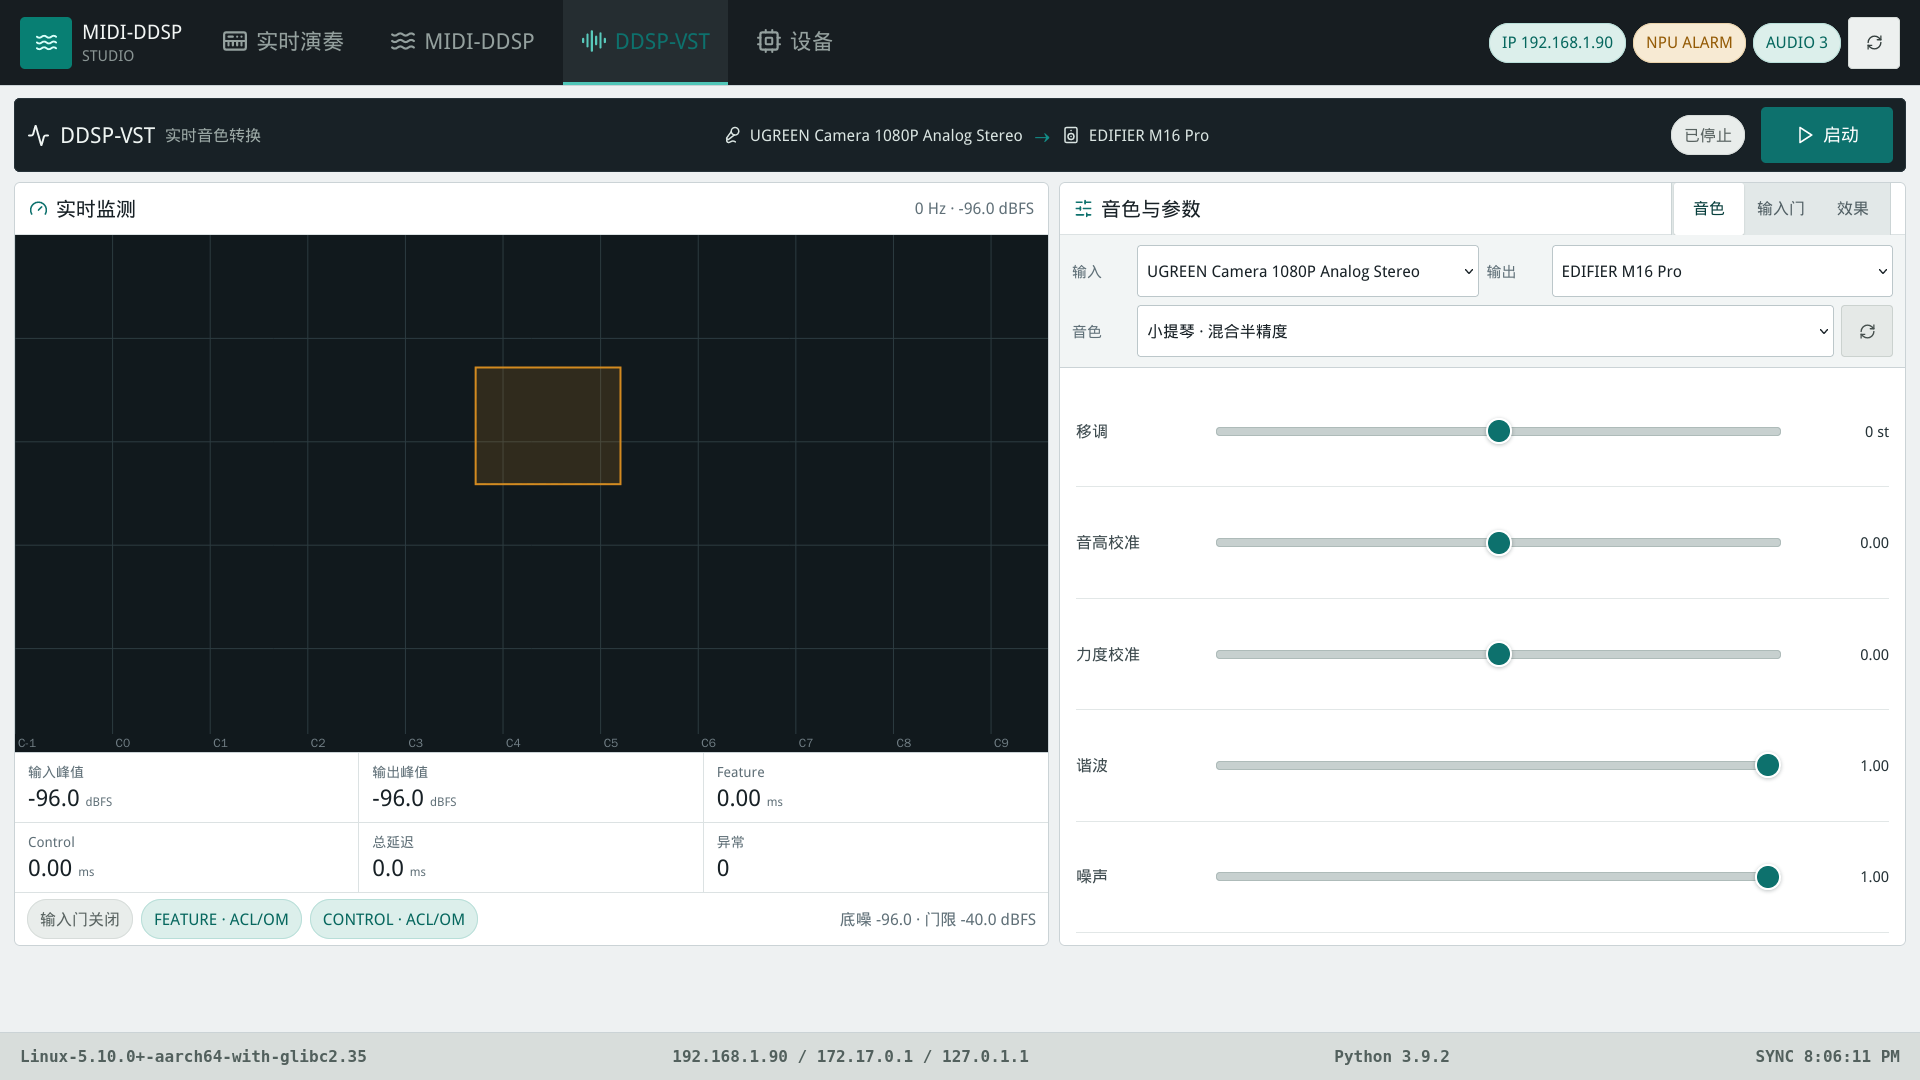
\includegraphics[keepaspectratio,alt={DDSP-VST 音色页面}]{cases/img3/case3-ui-ddsp-vst-tone.png}}
\caption{DDSP-VST 音色页面}
\end{figure}

{ % do not increment counter
\begin{longtable}[]{@{}
  >{\raggedright\arraybackslash}p{(\linewidth - 8\tabcolsep) * \real{0.2000}}
  >{\raggedright\arraybackslash}p{(\linewidth - 8\tabcolsep) * \real{0.2000}}
  >{\raggedright\arraybackslash}p{(\linewidth - 8\tabcolsep) * \real{0.2000}}
  >{\raggedright\arraybackslash}p{(\linewidth - 8\tabcolsep) * \real{0.2000}}
  >{\raggedright\arraybackslash}p{(\linewidth - 8\tabcolsep) * \real{0.2000}}@{}}
\toprule\noalign{}
\begin{minipage}[b]{\linewidth}\raggedright
区域
\end{minipage} & \begin{minipage}[b]{\linewidth}\raggedright
控件
\end{minipage} & \begin{minipage}[b]{\linewidth}\raggedright
作用
\end{minipage} & \begin{minipage}[b]{\linewidth}\raggedright
正常状态
\end{minipage} & \begin{minipage}[b]{\linewidth}\raggedright
注意事项
\end{minipage} \\
\midrule\noalign{}
\endhead
\bottomrule\noalign{}
\endlastfoot
顶部链路 & 输入、输出、运行/停止 & 明确真实设备路径 & UGREEN 到
EDIFIER，运行中 & 运行时不允许静默换设备 \\
轨迹 Canvas & 音高和响度点 & 观察单音输入与门限 & Canvas 非空，异常为 0
& 环境噪声也可能有音高估计，不等于已输出 \\
模型区 & 11 种中文音色 & 选择 Control OM & 小提琴混合半精度 &
后端仍用稳定模型 ID 和 SHA256 \\
音色参数 & 移调、音高校准、力度、谐波、噪声 & 调整转换控制 &
有边界值即时更新 & 谐波和噪声全关会失去主要声源 \\
指标 & Feature、Control、总延迟、后端 & 证明 OM 链路和线程状态 &
\passthrough{\lstinline!ACL/OM!} 且异常 0 & 指标不能代替听感评价 \\
\end{longtable}
}

\subsection{DDSP-VST 输入门}\label{src-experiment-case3-ui-vst-gate}

\begin{figure}
\centering
\pandocbounded{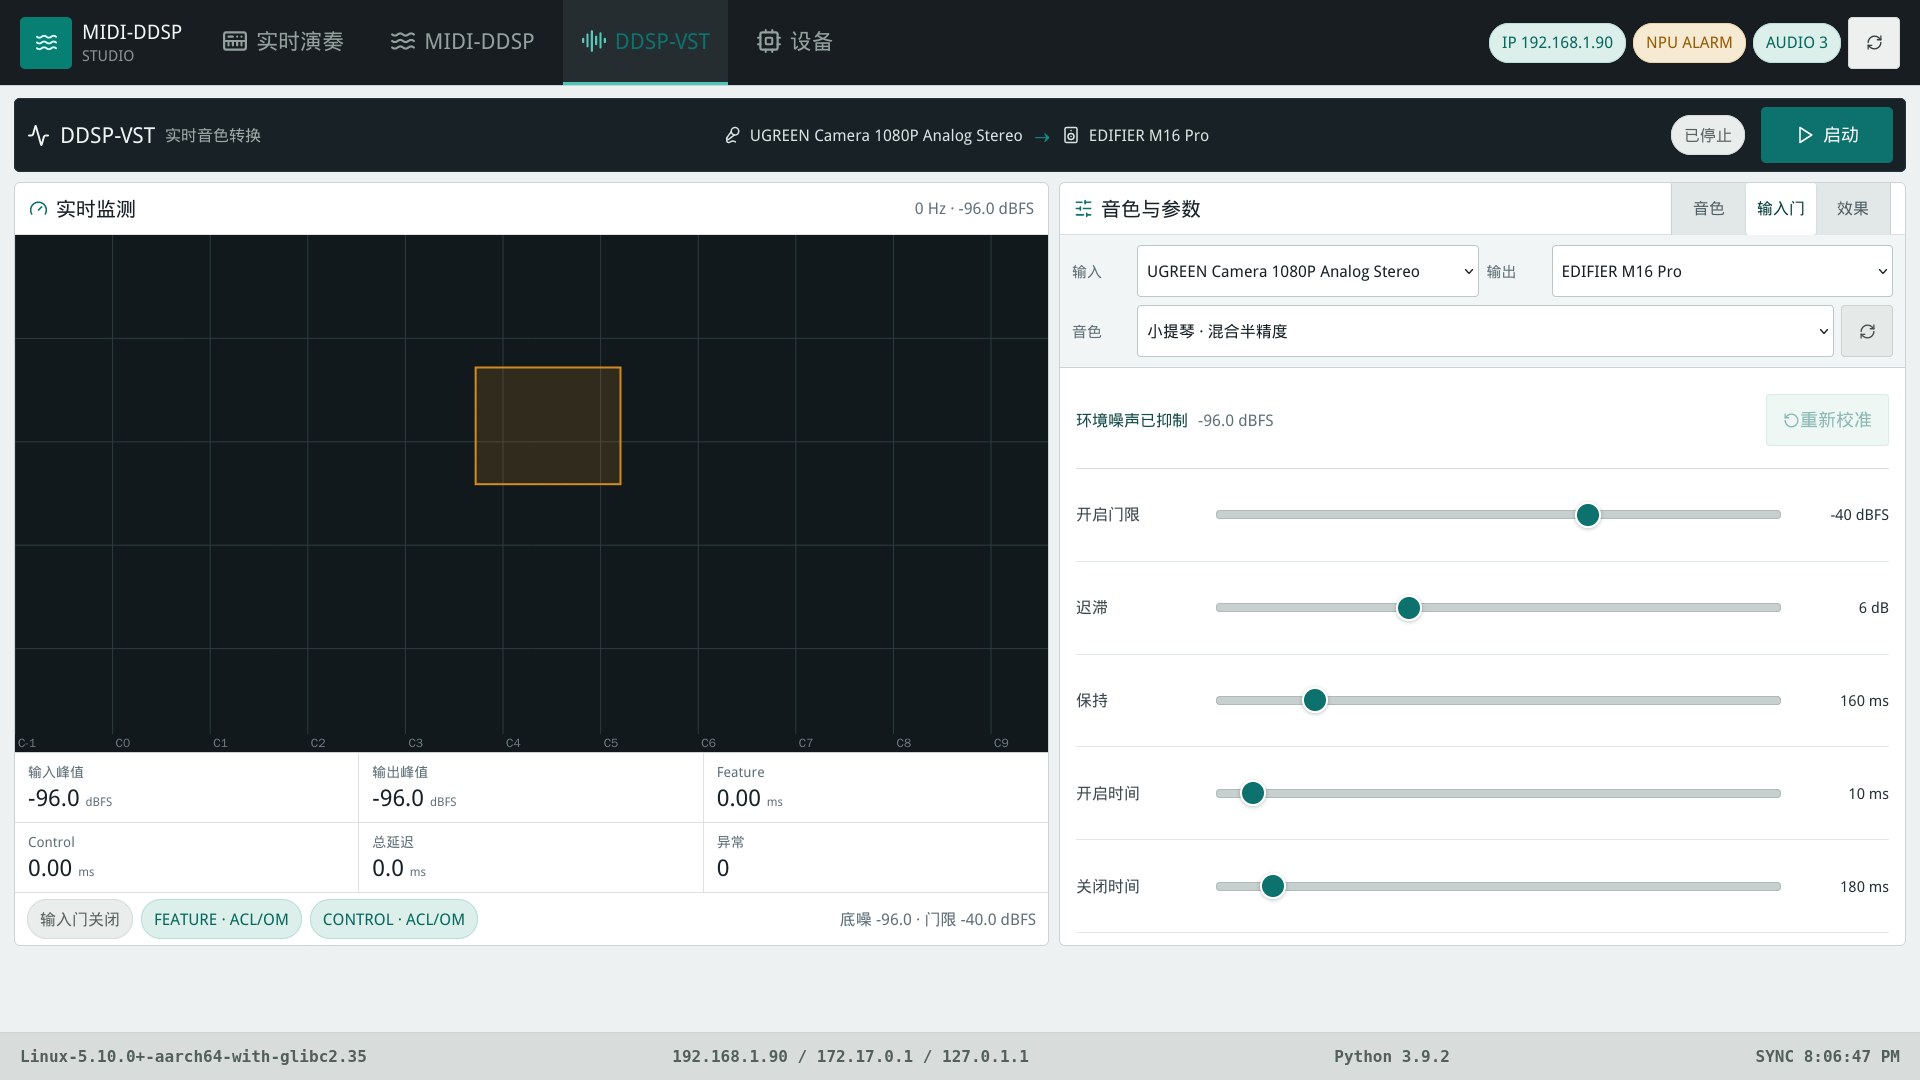
\includegraphics[keepaspectratio,alt={DDSP-VST 输入门页面}]{cases/img3/case3-ui-ddsp-vst-gate.png}}
\caption{DDSP-VST 输入门页面}
\end{figure}

{ % do not increment counter
\begin{longtable}[]{@{}
  >{\raggedright\arraybackslash}p{(\linewidth - 8\tabcolsep) * \real{0.2000}}
  >{\raggedright\arraybackslash}p{(\linewidth - 8\tabcolsep) * \real{0.2000}}
  >{\raggedright\arraybackslash}p{(\linewidth - 8\tabcolsep) * \real{0.2000}}
  >{\raggedright\arraybackslash}p{(\linewidth - 8\tabcolsep) * \real{0.2000}}
  >{\raggedright\arraybackslash}p{(\linewidth - 8\tabcolsep) * \real{0.2000}}@{}}
\toprule\noalign{}
\begin{minipage}[b]{\linewidth}\raggedright
区域
\end{minipage} & \begin{minipage}[b]{\linewidth}\raggedright
控件
\end{minipage} & \begin{minipage}[b]{\linewidth}\raggedright
作用
\end{minipage} & \begin{minipage}[b]{\linewidth}\raggedright
正常状态
\end{minipage} & \begin{minipage}[b]{\linewidth}\raggedright
注意事项
\end{minipage} \\
\midrule\noalign{}
\endhead
\bottomrule\noalign{}
\endlastfoot
校准 & 重新校准 & 采集环境底噪并给出建议门限 & 显示底噪和门限 &
校准时应保持安静，不要讲话或播放声音 \\
开启门限 & dBFS 滑块 & 达到阈值后允许音频进入 & 底噪低于开启门限 &
太低会被噪声触发，太高会吞轻声 \\
迟滞 & dB 滑块 & 让关闭阈值低于开启阈值 & 开关不频繁抖动 &
迟滞不是额外增益 \\
保持/开启/关闭 & 毫秒滑块 & 平滑门状态 & 输入门状态稳定 &
关闭过慢会拖尾，过快会切断音头 \\
状态条 & 输入门已关闭/打开 & 明确当前是否输出 & 静音环境显示关闭 &
有音高点但门关闭时不会送入合成输出 \\
\end{longtable}
}

\subsection{DDSP-VST 效果}\label{src-experiment-case3-ui-vst-effects}

\begin{figure}
\centering
\pandocbounded{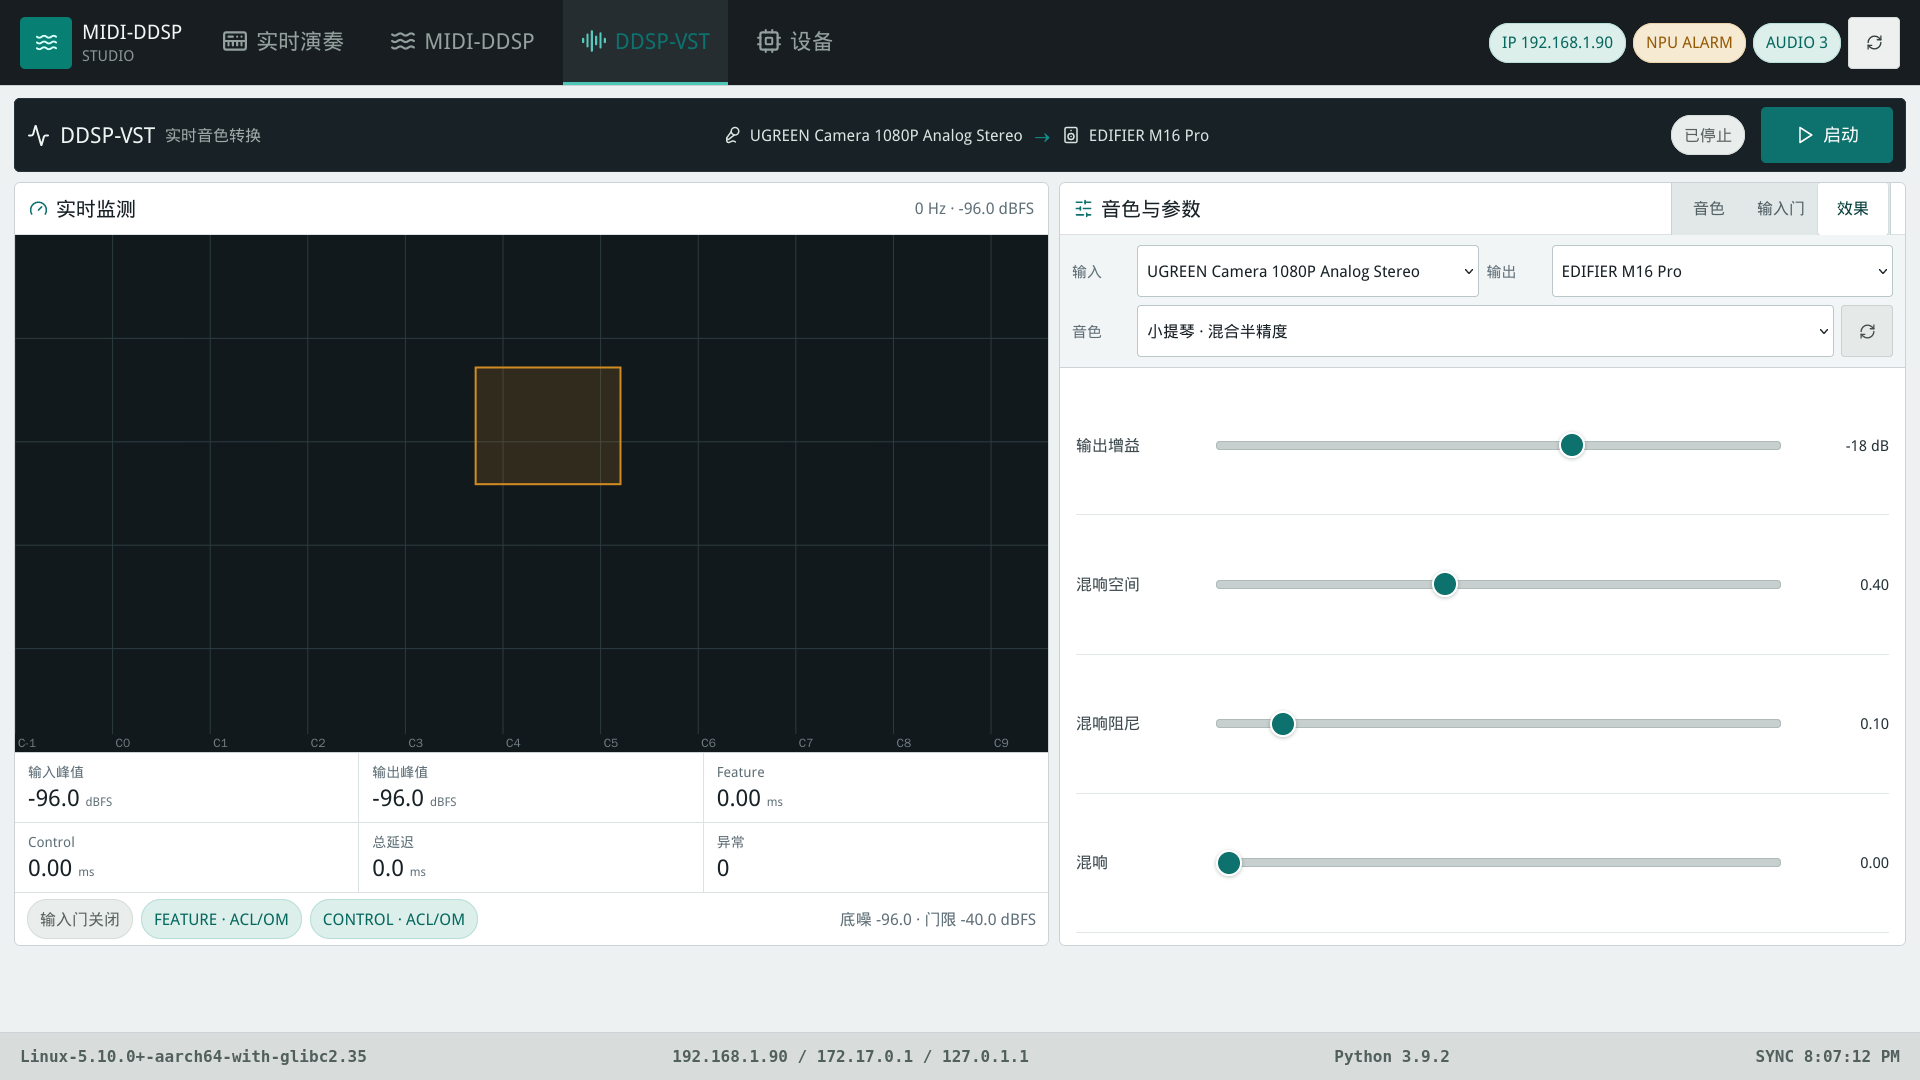
\includegraphics[keepaspectratio,alt={DDSP-VST 效果页面}]{cases/img3/case3-ui-ddsp-vst-effects.png}}
\caption{DDSP-VST 效果页面}
\end{figure}

{ % do not increment counter
\begin{longtable}[]{@{}
  >{\raggedright\arraybackslash}p{(\linewidth - 8\tabcolsep) * \real{0.2000}}
  >{\raggedright\arraybackslash}p{(\linewidth - 8\tabcolsep) * \real{0.2000}}
  >{\raggedright\arraybackslash}p{(\linewidth - 8\tabcolsep) * \real{0.2000}}
  >{\raggedright\arraybackslash}p{(\linewidth - 8\tabcolsep) * \real{0.2000}}
  >{\raggedright\arraybackslash}p{(\linewidth - 8\tabcolsep) * \real{0.2000}}@{}}
\toprule\noalign{}
\begin{minipage}[b]{\linewidth}\raggedright
区域
\end{minipage} & \begin{minipage}[b]{\linewidth}\raggedright
控件
\end{minipage} & \begin{minipage}[b]{\linewidth}\raggedright
作用
\end{minipage} & \begin{minipage}[b]{\linewidth}\raggedright
正常状态
\end{minipage} & \begin{minipage}[b]{\linewidth}\raggedright
注意事项
\end{minipage} \\
\midrule\noalign{}
\endhead
\bottomrule\noalign{}
\endlastfoot
输出增益 & dB 滑块 & 控制转换后 PCM & 默认
\passthrough{\lstinline!-18 dB!} & 与系统音量分离，避免同时放大两处 \\
混响空间 & 0 到 1 & 调整房间反馈感 & 默认 0.40 &
更大空间会增加主观尾音 \\
混响阻尼 & 0 到 1 & 衰减高频反馈 & 默认 0.10 &
不是低通滤波器的精确截止频率 \\
混响 & 0 到 1 & 控制湿声比例 & 默认 0 & 第一版没有原声 Dry/Wet 直通 \\
安全状态 & 异常和安全静音 & 防止持续过载 & 异常 0、安全静音关闭 &
触发后应停止并排查输入和增益 \\
\end{longtable}
}

\subsection{设备概览}\label{src-experiment-case3-ui-device-overview}

\begin{figure}
\centering
\pandocbounded{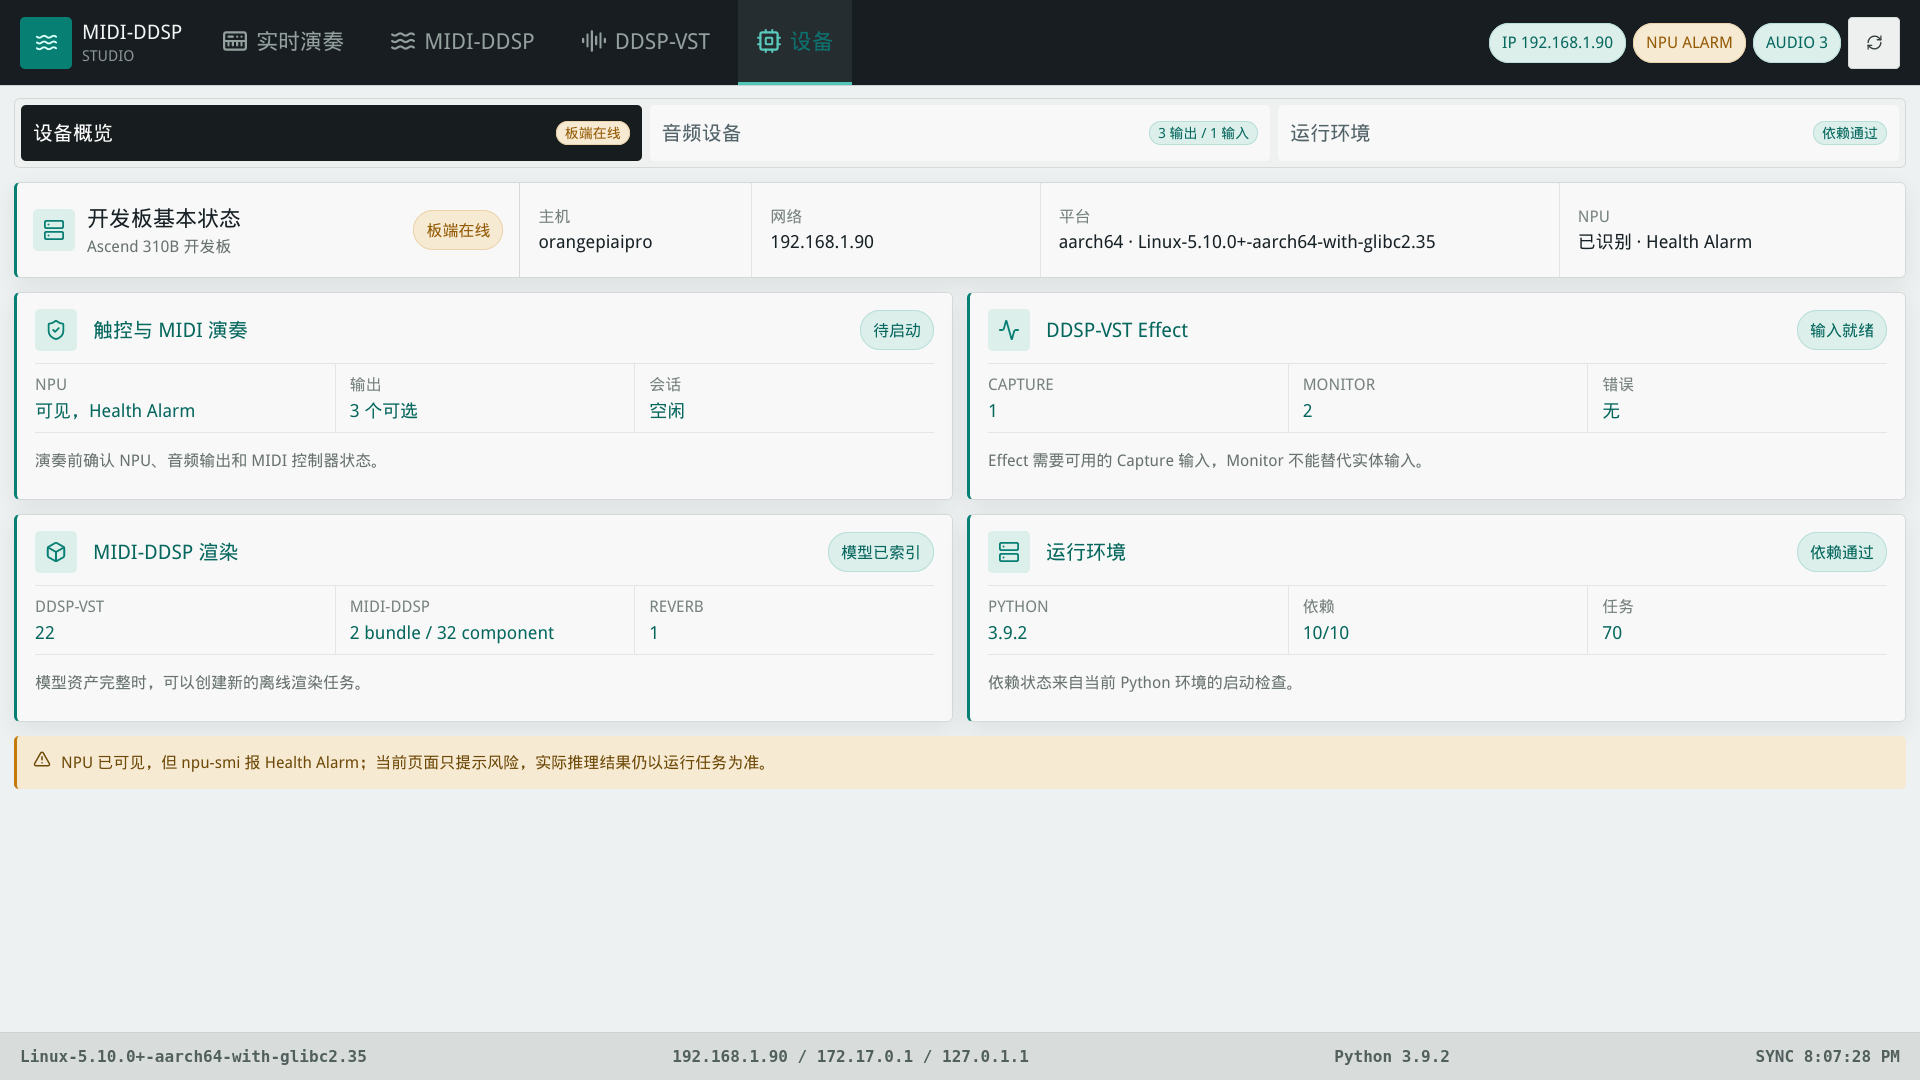
\includegraphics[keepaspectratio,alt={设备概览页面}]{cases/img3/case3-ui-devices-overview.png}}
\caption{设备概览页面}
\end{figure}

\clearpage

{ % do not increment counter
\begin{longtable}[]{@{}
  >{\raggedright\arraybackslash}p{(\linewidth - 4\tabcolsep) * \real{0.3333}}
  >{\raggedright\arraybackslash}p{(\linewidth - 4\tabcolsep) * \real{0.3333}}
  >{\raggedright\arraybackslash}p{(\linewidth - 4\tabcolsep) * \real{0.3333}}@{}}
\toprule\noalign{}
\begin{minipage}[b]{\linewidth}\raggedright
区域
\end{minipage} & \begin{minipage}[b]{\linewidth}\raggedright
正常状态
\end{minipage} & \begin{minipage}[b]{\linewidth}\raggedright
验收要点
\end{minipage} \\
\midrule\noalign{}
\endhead
\bottomrule\noalign{}
\endlastfoot
开发板状态 & 板端在线、IP 可见、NPU 状态显示 & Health Alarm
是警告，真实推理结果优先 \\
触控与 MIDI & 输出可选、会话无错误 &
概览只提示准备度，不重复提供跳转按钮 \\
DDSP-VST & 至少一个 capture、错误为 0 & monitor 数量不代表麦克风数量 \\
MIDI-DDSP & bundle 和组件已索引 & 发现资产不等同于已听音验收 \\
运行环境 & Python、依赖、任务状态可见 & 详细内容放在运行环境页 \\
\end{longtable}
}

\subsection{音频输出与扬声器测试}\label{src-experiment-case3-ui-audio-output}

\begin{figure}
\centering
\pandocbounded{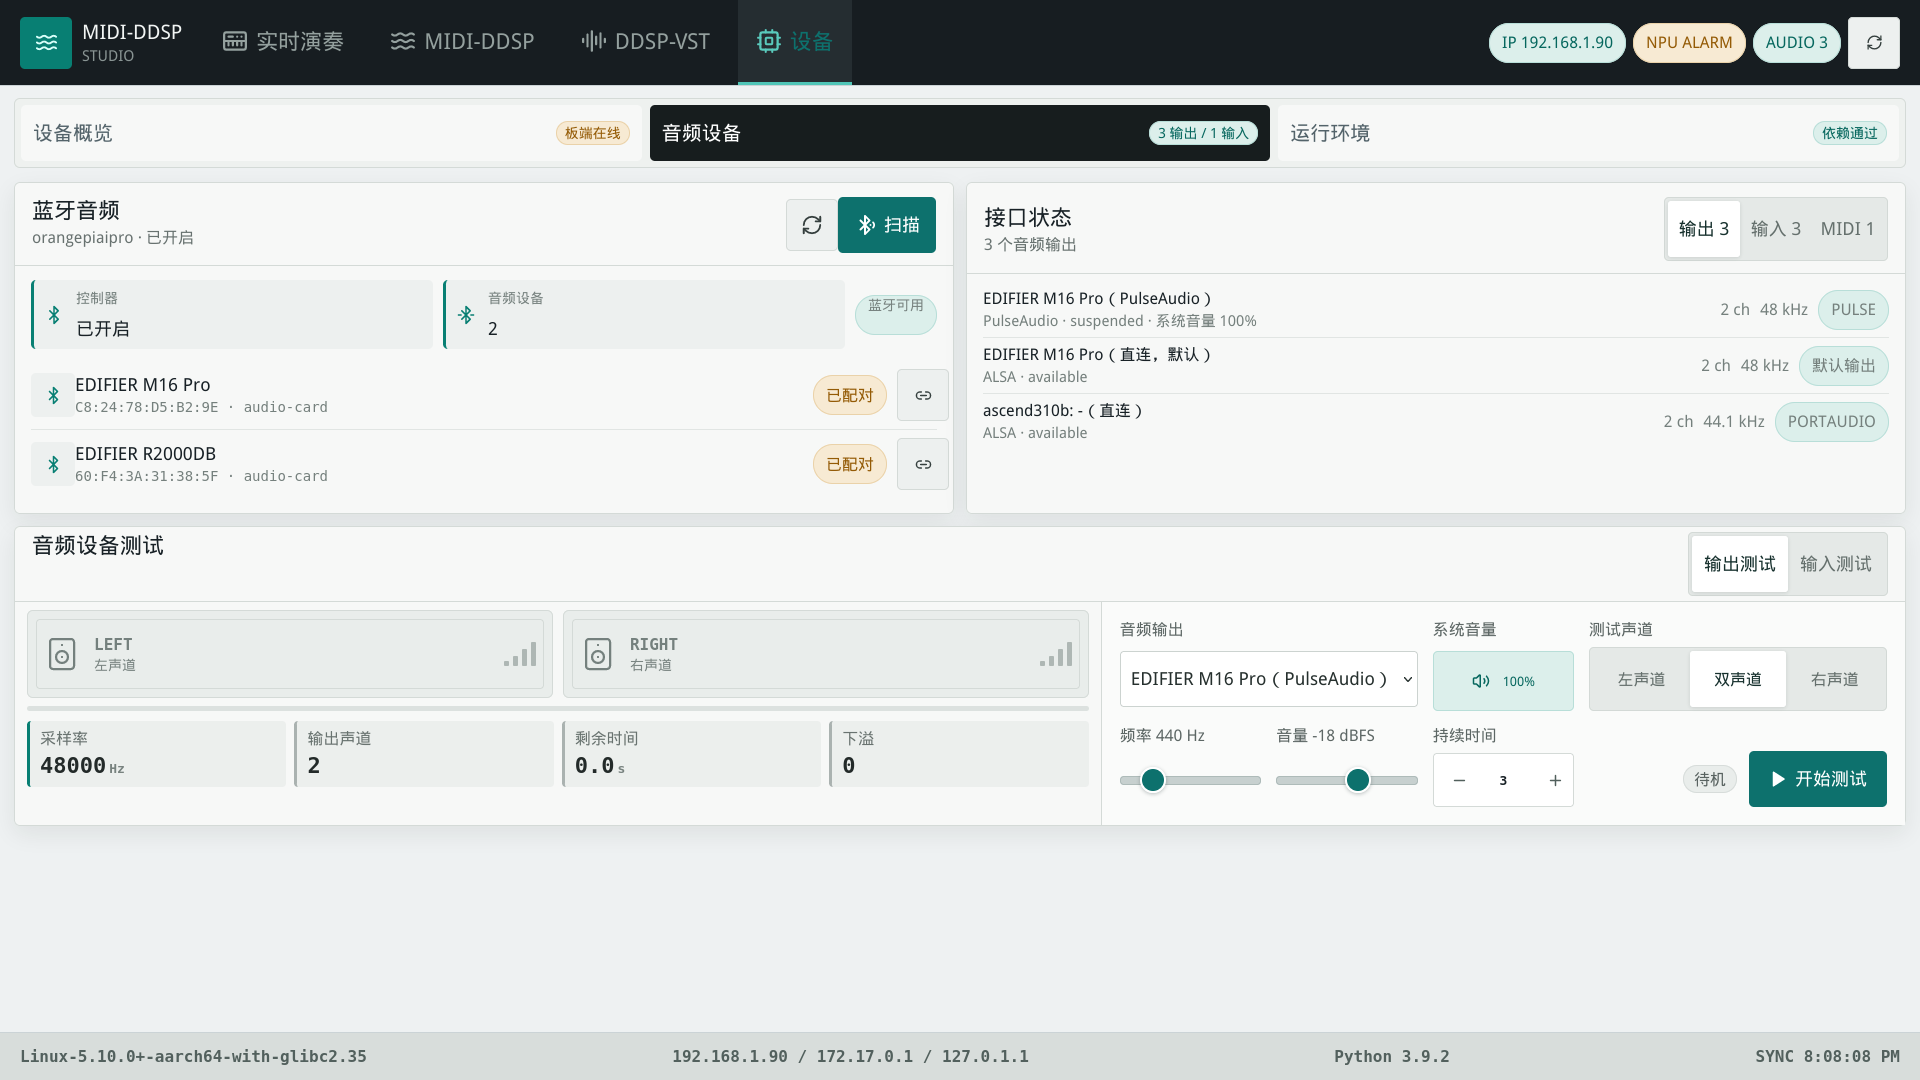
\includegraphics[keepaspectratio,alt={音频输出与扬声器测试页面}]{cases/img3/case3-ui-devices-audio-output.png}}
\caption{音频输出与扬声器测试页面}
\end{figure}

{ % do not increment counter
\begin{longtable}[]{@{}
  >{\raggedright\arraybackslash}p{(\linewidth - 8\tabcolsep) * \real{0.2000}}
  >{\raggedright\arraybackslash}p{(\linewidth - 8\tabcolsep) * \real{0.2000}}
  >{\raggedright\arraybackslash}p{(\linewidth - 8\tabcolsep) * \real{0.2000}}
  >{\raggedright\arraybackslash}p{(\linewidth - 8\tabcolsep) * \real{0.2000}}
  >{\raggedright\arraybackslash}p{(\linewidth - 8\tabcolsep) * \real{0.2000}}@{}}
\toprule\noalign{}
\begin{minipage}[b]{\linewidth}\raggedright
区域
\end{minipage} & \begin{minipage}[b]{\linewidth}\raggedright
控件
\end{minipage} & \begin{minipage}[b]{\linewidth}\raggedright
作用
\end{minipage} & \begin{minipage}[b]{\linewidth}\raggedright
正常状态
\end{minipage} & \begin{minipage}[b]{\linewidth}\raggedright
注意事项
\end{minipage} \\
\midrule\noalign{}
\endhead
\bottomrule\noalign{}
\endlastfoot
蓝牙音频 & 刷新、扫描、连接 & 管理板端已有蓝牙能力 &
控制器开启、设备可见 & 不在板端安装缺失的
\passthrough{\lstinline!bluetoothctl!} \\
接口状态 & 输出/输入/MIDI & 切换设备清单 & EDIFIER PulseAudio 和直接
ALSA 可见 & ``检测到''不等于已听见 \\
声道表 & Left、Right 和电平 & 展示测试声道和状态 & 空闲时电平归零 &
测试会独占输出资源 \\
输出设置 & 音频输出、系统音量 & 选择 sink 并显示真实系统音量 &
EDIFIER、100\%、未静音 & 音箱硬件按键应通过设备事件更新显示 \\
测试设置 & 左/双/右声道、频率、增益、时长 & 播放受控正弦测试 & 状态从
IDLE 进入运行 & 从低增益开始，避免突然高声压 \\
\end{longtable}
}

\subsection{音频输入与麦克风测试}\label{src-experiment-case3-ui-audio-input}

\begin{figure}
\centering
\pandocbounded{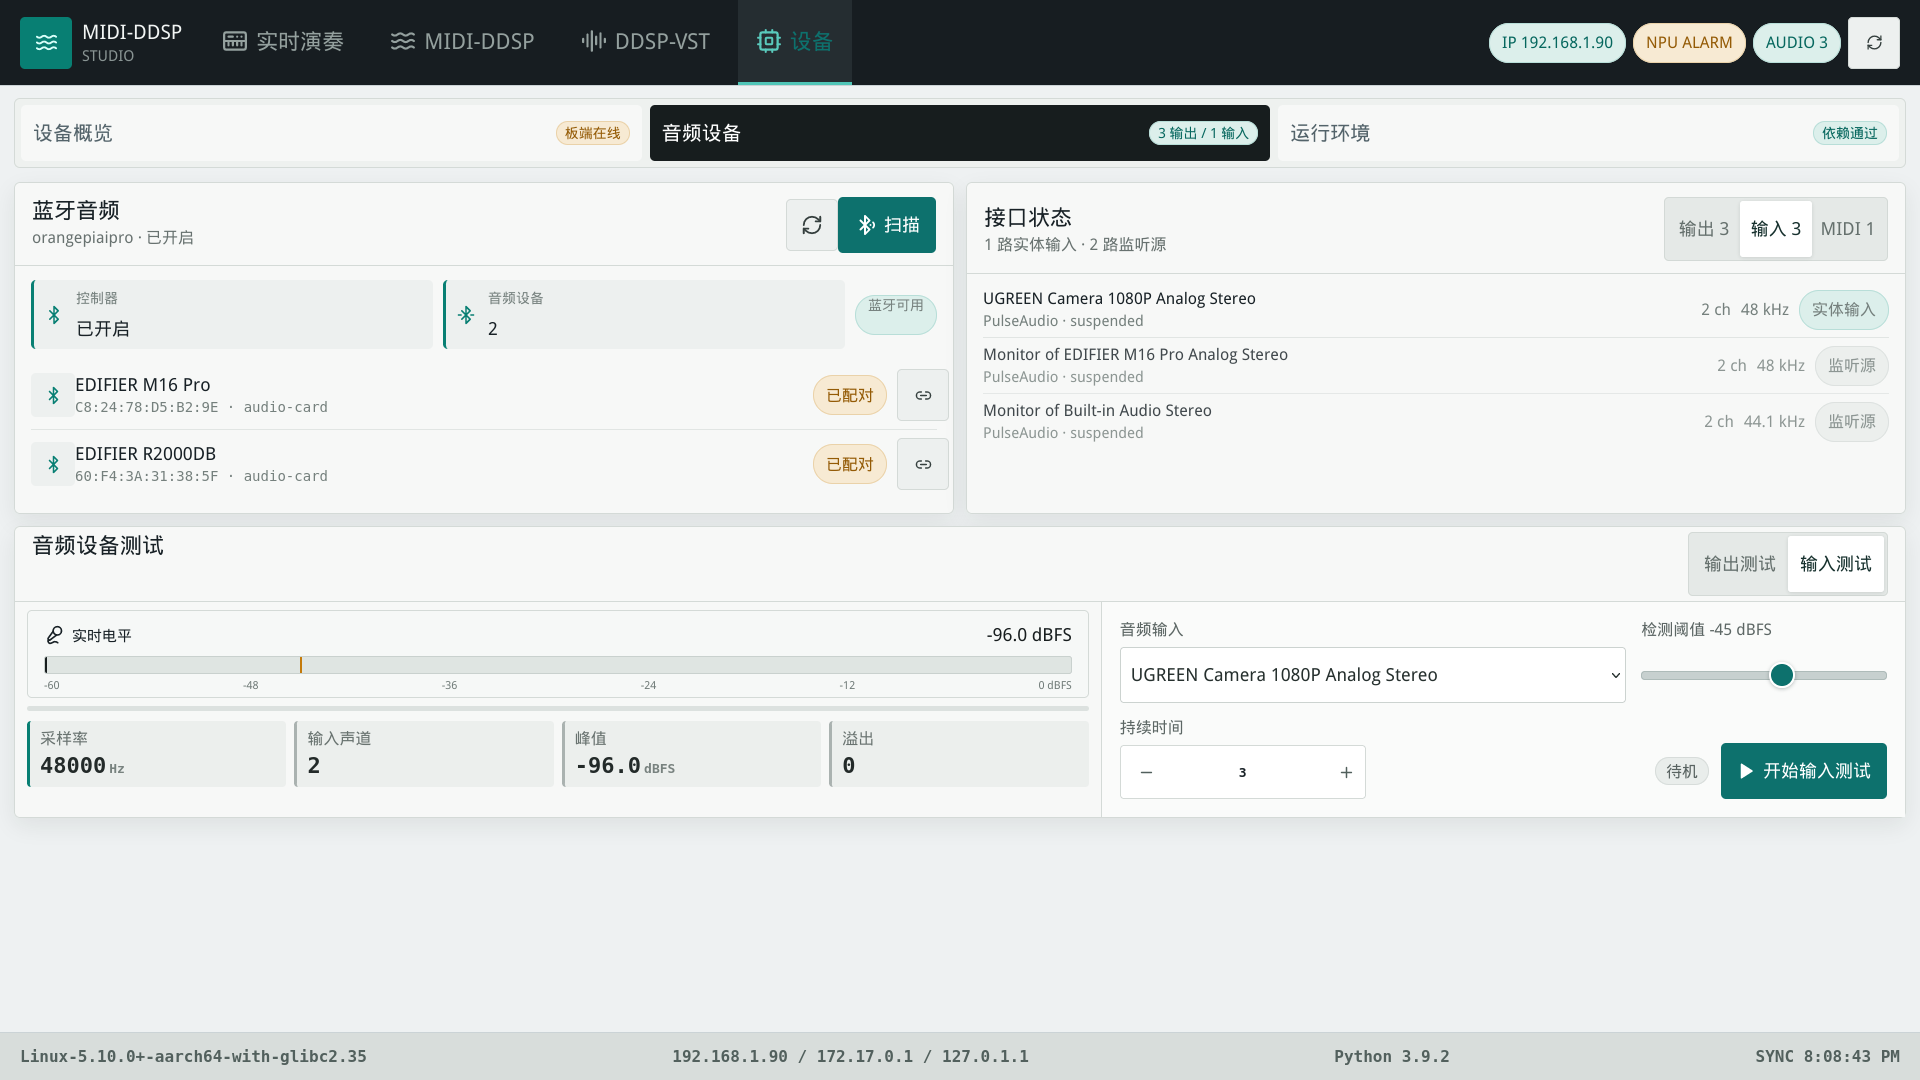
\includegraphics[keepaspectratio,alt={音频输入与麦克风测试页面}]{cases/img3/case3-ui-devices-audio-input.png}}
\caption{音频输入与麦克风测试页面}
\end{figure}

{ % do not increment counter
\begin{longtable}[]{@{}
  >{\raggedright\arraybackslash}p{(\linewidth - 8\tabcolsep) * \real{0.2000}}
  >{\raggedright\arraybackslash}p{(\linewidth - 8\tabcolsep) * \real{0.2000}}
  >{\raggedright\arraybackslash}p{(\linewidth - 8\tabcolsep) * \real{0.2000}}
  >{\raggedright\arraybackslash}p{(\linewidth - 8\tabcolsep) * \real{0.2000}}
  >{\raggedright\arraybackslash}p{(\linewidth - 8\tabcolsep) * \real{0.2000}}@{}}
\toprule\noalign{}
\begin{minipage}[b]{\linewidth}\raggedright
区域
\end{minipage} & \begin{minipage}[b]{\linewidth}\raggedright
控件
\end{minipage} & \begin{minipage}[b]{\linewidth}\raggedright
作用
\end{minipage} & \begin{minipage}[b]{\linewidth}\raggedright
正常状态
\end{minipage} & \begin{minipage}[b]{\linewidth}\raggedright
注意事项
\end{minipage} \\
\midrule\noalign{}
\endhead
\bottomrule\noalign{}
\endlastfoot
输入清单 & capture 与 monitor & 区分实体采集和回放监视 & UGREEN 标为
CAPTURE & Effect 和输入测试都拒绝 monitor \\
实时电平 & dBFS 表和峰值 & 观察麦克风输入 & 讲话时电平变化、无溢出 &
\passthrough{\lstinline!-96 dBFS!} 表示空闲或未开始测试 \\
输入选择 & capture 下拉 & 固定真实麦克风 ID & UGREEN 被选中 &
设备断开后不会自动替换 \\
检测阈值 & dBFS 滑块 & 控制输入测试是否判为有效 & 高于底噪、低于说话峰值
& 与 DDSP-VST 噪声门是两个不同设置 \\
时长与开始 & 步进器、开始输入测试 & 运行独占采集检查 & IDLE 或完成结果 &
测试期间不能启动 Effect \\
\end{longtable}
}

\subsection{MIDI 设备}\label{src-experiment-case3-ui-midi-device}

\begin{figure}
\centering
\pandocbounded{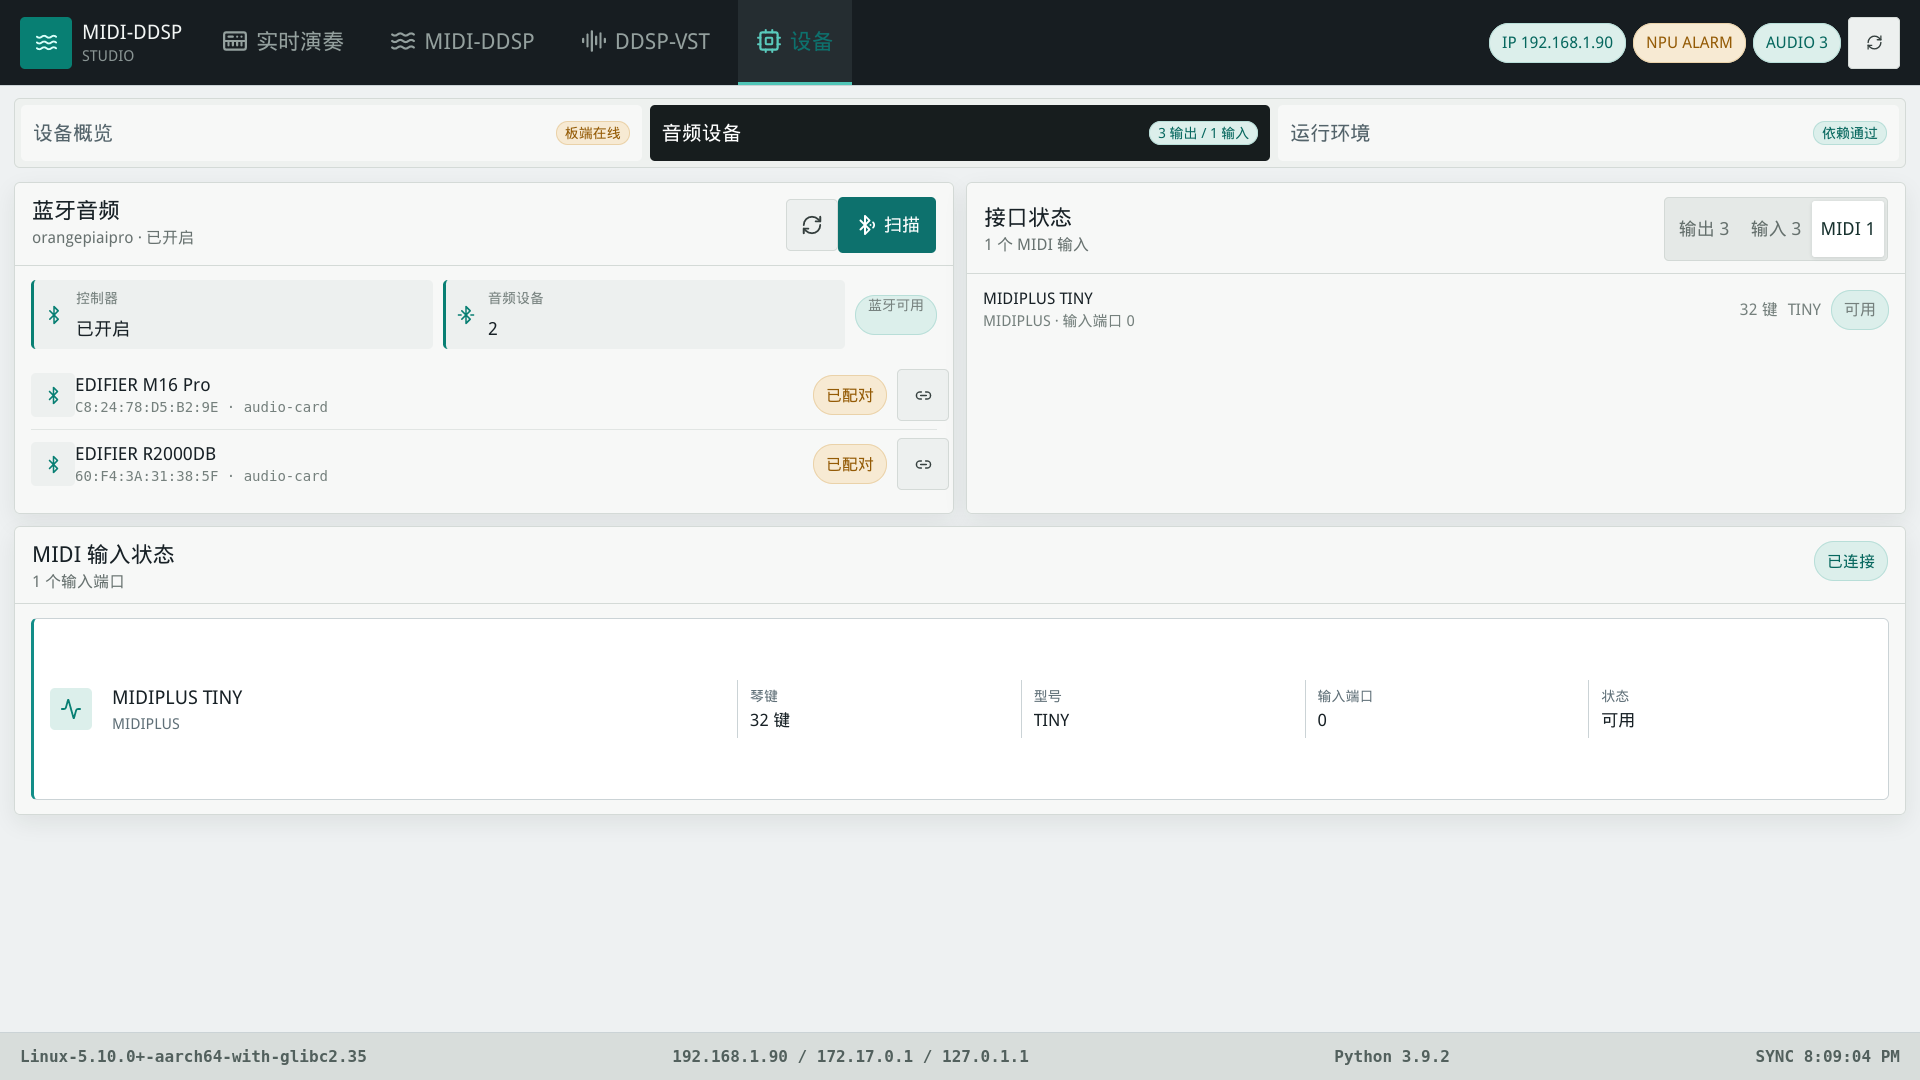
\includegraphics[keepaspectratio,alt={MIDI 设备页面}]{cases/img3/case3-ui-devices-midi.png}}
\caption{MIDI 设备页面}
\end{figure}

{ % do not increment counter
\begin{longtable}[]{@{}
  >{\raggedright\arraybackslash}p{(\linewidth - 8\tabcolsep) * \real{0.2000}}
  >{\raggedright\arraybackslash}p{(\linewidth - 8\tabcolsep) * \real{0.2000}}
  >{\raggedright\arraybackslash}p{(\linewidth - 8\tabcolsep) * \real{0.2000}}
  >{\raggedright\arraybackslash}p{(\linewidth - 8\tabcolsep) * \real{0.2000}}
  >{\raggedright\arraybackslash}p{(\linewidth - 8\tabcolsep) * \real{0.2000}}@{}}
\toprule\noalign{}
\begin{minipage}[b]{\linewidth}\raggedright
区域
\end{minipage} & \begin{minipage}[b]{\linewidth}\raggedright
控件
\end{minipage} & \begin{minipage}[b]{\linewidth}\raggedright
作用
\end{minipage} & \begin{minipage}[b]{\linewidth}\raggedright
正常状态
\end{minipage} & \begin{minipage}[b]{\linewidth}\raggedright
注意事项
\end{minipage} \\
\midrule\noalign{}
\endhead
\bottomrule\noalign{}
\endlastfoot
MIDI 清单 & MIDI 页签 & 枚举服务端输入端口 & MIDIPLUS TINY、32
keys、AVAILABLE & 浏览器 Web MIDI 不是板端输入来源 \\
制造商与端口 & 型号、Input port & 识别正确设备 & MIDIPLUS、端口 0 &
重新插拔后设备 ID 可能变化，应刷新 \\
MIDI 输入状态 & 全宽设备状态卡 & 显示键数、型号、输入端口和可用状态 &
MIDIPLUS TINY 已连接 & 切换到 MIDI 后不显示输入或输出音频测试；MIDI
枚举本身不会产生声音 \\
蓝牙区 & 已配对音频设备 & 展示另一类外设状态 & 与 MIDI 清单分开 &
蓝牙音频不能替代 USB MIDI \\
\end{longtable}
}

\subsection{运行环境}\label{src-experiment-case3-ui-runtime}

\begin{figure}
\centering
\pandocbounded{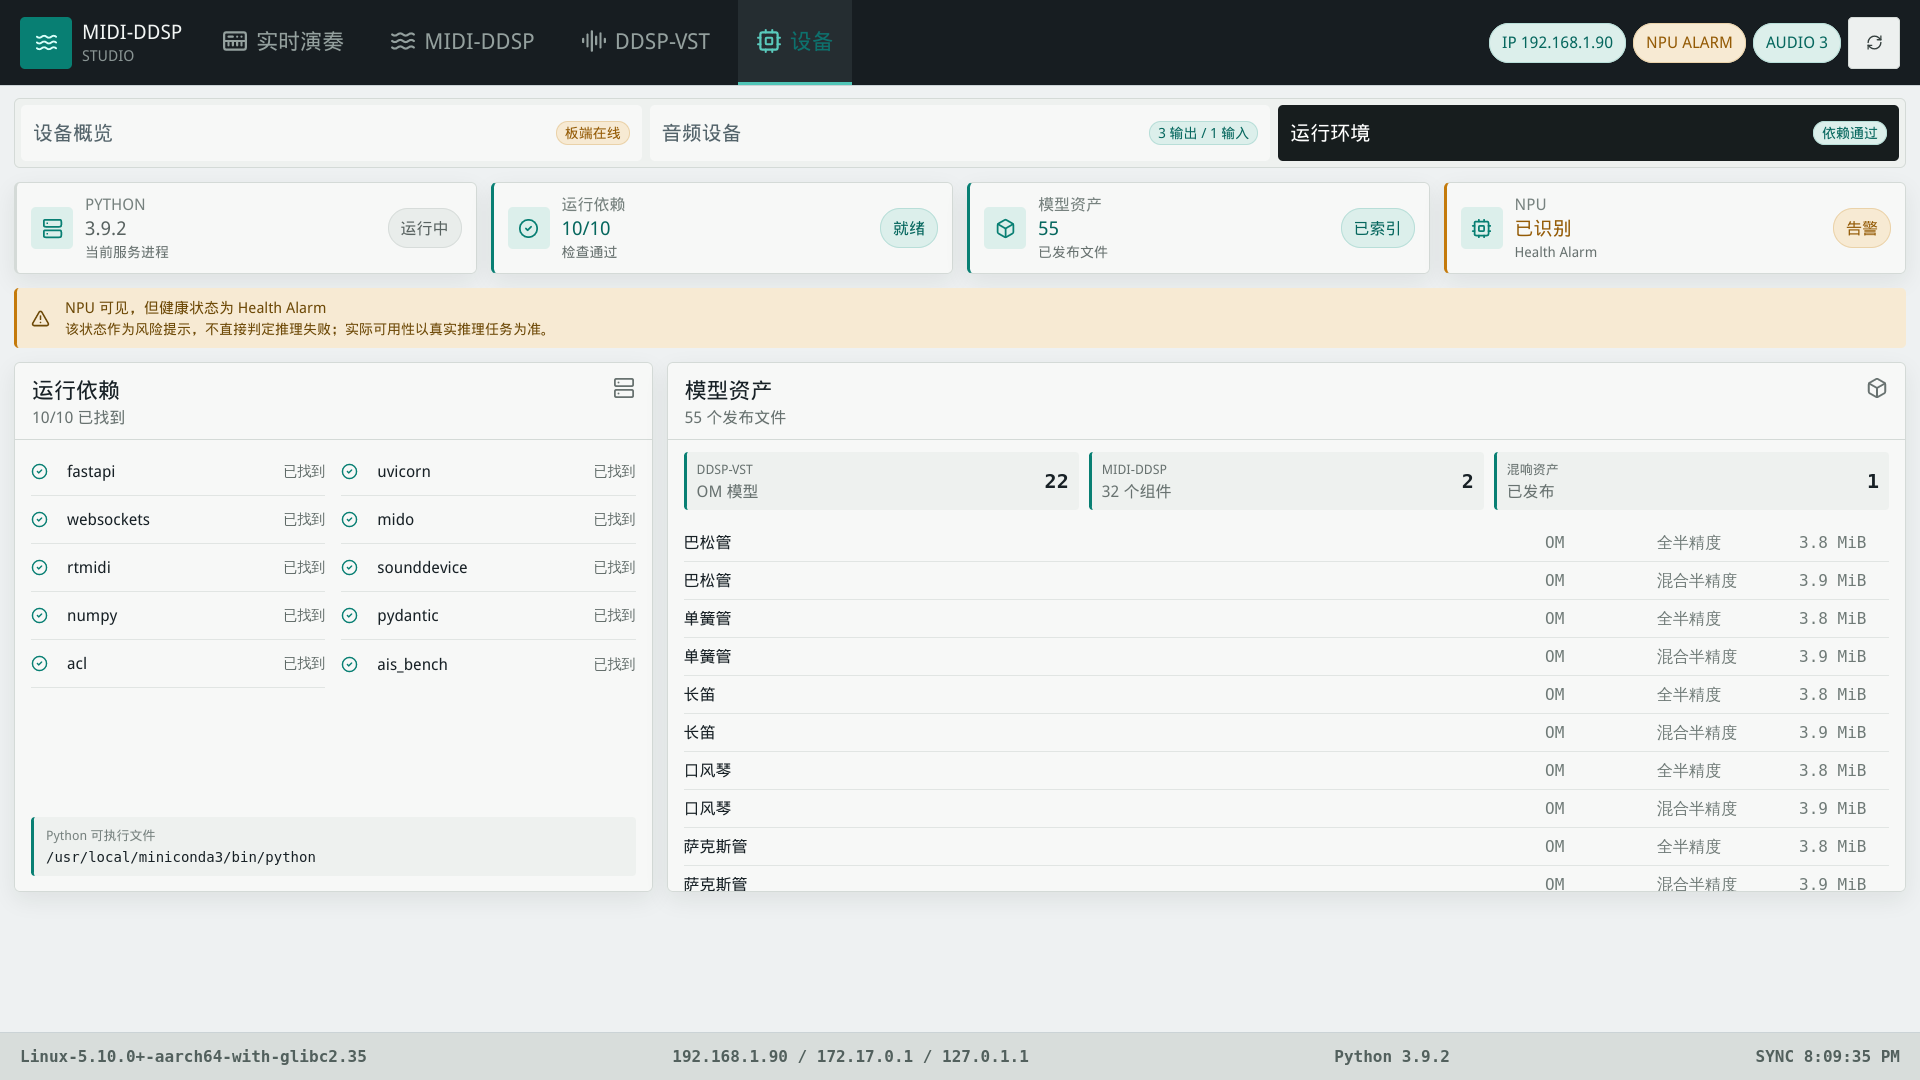
\includegraphics[keepaspectratio,alt={运行环境页面}]{cases/img3/case3-ui-devices-runtime.png}}
\caption{运行环境页面}
\end{figure}

\clearpage

{ % do not increment counter
\begin{longtable}[]{@{}
  >{\raggedright\arraybackslash}p{(\linewidth - 8\tabcolsep) * \real{0.2000}}
  >{\raggedright\arraybackslash}p{(\linewidth - 8\tabcolsep) * \real{0.2000}}
  >{\raggedright\arraybackslash}p{(\linewidth - 8\tabcolsep) * \real{0.2000}}
  >{\raggedright\arraybackslash}p{(\linewidth - 8\tabcolsep) * \real{0.2000}}
  >{\raggedright\arraybackslash}p{(\linewidth - 8\tabcolsep) * \real{0.2000}}@{}}
\toprule\noalign{}
\begin{minipage}[b]{\linewidth}\raggedright
区域
\end{minipage} & \begin{minipage}[b]{\linewidth}\raggedright
控件
\end{minipage} & \begin{minipage}[b]{\linewidth}\raggedright
作用
\end{minipage} & \begin{minipage}[b]{\linewidth}\raggedright
正常状态
\end{minipage} & \begin{minipage}[b]{\linewidth}\raggedright
注意事项
\end{minipage} \\
\midrule\noalign{}
\endhead
\bottomrule\noalign{}
\endlastfoot
摘要 & Python、依赖、模型、NPU & 一屏判断服务准备度 & Python
3.9.2、10/10 依赖 & 版本以当前板端环境为准 \\
NPU 警告 & Health Alarm 文本 & 如实展示硬件诊断 & 警告可见 &
不直接粘贴整个终端输出 \\
运行依赖 & 包名与找到状态 & 定位 Python 启动缺包 & 全部找到 &
板端只允许唯一 requirements 的 pip 安装例外 \\
模型资产 & 类型、精度、大小 & 检查目录索引结果 & OM 数量和精度可见 &
资产存在仍需哈希和真实推理验证 \\
Python 路径 & 可执行文件 & 证明使用现有 conda base &
\passthrough{\lstinline!/usr/local/miniconda3/bin/python!} &
不回退到系统 Python \\
\end{longtable}
}

\subsection{已验证视口}\label{src-experiment-case3-viewport-matrix}

{ % do not increment counter
\begin{longtable}[]{@{}
  >{\raggedright\arraybackslash}p{(\linewidth - 6\tabcolsep) * \real{0.2500}}
  >{\raggedright\arraybackslash}p{(\linewidth - 6\tabcolsep) * \real{0.2500}}
  >{\raggedright\arraybackslash}p{(\linewidth - 6\tabcolsep) * \real{0.2500}}
  >{\raggedright\arraybackslash}p{(\linewidth - 6\tabcolsep) * \real{0.2500}}@{}}
\toprule\noalign{}
\begin{minipage}[b]{\linewidth}\raggedright
视口
\end{minipage} & \begin{minipage}[b]{\linewidth}\raggedright
输入方式
\end{minipage} & \begin{minipage}[b]{\linewidth}\raggedright
导航
\end{minipage} & \begin{minipage}[b]{\linewidth}\raggedright
重点验收
\end{minipage} \\
\midrule\noalign{}
\endhead
\bottomrule\noalign{}
\endlastfoot
\passthrough{\lstinline!1920 x 1080!} & 10 英寸物理 kiosk & 完整顶部导航
& 12 张真实页面截图、实际点按、底部琴键贴边和无裁切 \\
\passthrough{\lstinline!1920 x 969!} & 10 英寸触摸内容视口 &
完整顶部导航 & 一屏主工作流、触控目标、Canvas 非空、无滚动冲突 \\
\passthrough{\lstinline!1366 x 768!} & 桌面 & 完整顶部导航 &
紧凑布局、无重叠和横向溢出 \\
\passthrough{\lstinline!1024 x 768!} & 平板 & 响应式顶部/底部策略 &
参数换行、可访问页签和触控尺寸 \\
\passthrough{\lstinline!390 x 844!} & 手机 & 底部导航 &
安全区、折叠内容、无文档级横向滚动 \\
\end{longtable}
}

\section{10. 从零复现实验}\label{src-experiment-case3-reproduction}

\subsection{接线与启动检查}\label{src-experiment-case3-bringup}

\begin{enumerate}
\def\labelenumi{\arabic{enumi}.}
\tightlist
\item
  断电状态连接开发板电源、启动存储、HDMI 屏幕和 USB 触控线。
\item
  连接 EDIFIER M16 Pro、UGREEN 摄像头和 MIDIPLUS TINY；高功耗 USB
  设备较多时使用合规的独立供电 Hub。
\item
  连接网线或 Wi-Fi，启动开发板，确认触摸和桌面正常。
\item
  在开发板查看 IPv4、USB、ALSA/PulseAudio 和
  MIDI；这些是板端只读诊断，不在开发电脑执行。
\end{enumerate}

\begin{lstlisting}[language=bash]
ip -4 address
lsusb
pactl list short sinks
pactl list short sources
cat /proc/asound/cards
cat /proc/asound/seq/clients
\end{lstlisting}

在 \passthrough{\lstinline!pactl list short sources!} 中，UGREEN
应出现为 \passthrough{\lstinline!alsa\_input...!} 实体
capture。\passthrough{\lstinline!*.monitor!} 是输出回放监视源，不能用于
DDSP-VST 或麦克风输入测试。

\subsection{开发电脑准备与本地测试}\label{src-experiment-case3-local-setup}

\begin{lstlisting}
cd D:\Github\Ascend310\samples\case3
python -m pip install -r requirements.txt
python -m pytest -q

cd webui
npm ci
npm run test
npm run build
npm run test:e2e
\end{lstlisting}

各 npm 命令的职责不同：

{ % do not increment counter
\begin{longtable}[]{@{}
  >{\raggedright\arraybackslash}p{(\linewidth - 4\tabcolsep) * \real{0.3333}}
  >{\raggedright\arraybackslash}p{(\linewidth - 4\tabcolsep) * \real{0.3333}}
  >{\raggedright\arraybackslash}p{(\linewidth - 4\tabcolsep) * \real{0.3333}}@{}}
\toprule\noalign{}
\begin{minipage}[b]{\linewidth}\raggedright
命令
\end{minipage} & \begin{minipage}[b]{\linewidth}\raggedright
作用
\end{minipage} & \begin{minipage}[b]{\linewidth}\raggedright
何时必须执行
\end{minipage} \\
\midrule\noalign{}
\endhead
\bottomrule\noalign{}
\endlastfoot
\passthrough{\lstinline!npm ci!} & 严格按
\passthrough{\lstinline!package-lock.json!} 安装前端依赖 &
第一次准备环境、删除过 \passthrough{\lstinline!node\_modules!}
或锁文件变化后 \\
\passthrough{\lstinline!npm run test!} & 用 Vitest
检查组件、状态和交互回归 &
前端逻辑、组件或相关样式改变后；纯低风险文字修改可酌情跳过 \\
\passthrough{\lstinline!npm run build!} & TypeScript 检查并生成部署所需
\passthrough{\lstinline!webui/dist!} & 任何前端源码变化后必须执行 \\
\passthrough{\lstinline!npm run test:e2e!} & 用 Playwright
检查真实页面布局和交互 & 发布前或影响工作流、响应式、Canvas 时 \\
\end{longtable}
}

开发板不安装 Node 或 npm，也不运行 Vite
生产服务器。它只接收开发电脑生成的
\passthrough{\lstinline!webui/dist/!}。

\subsection{下载、校验和准备模型}\label{src-experiment-case3-prepare-models}

先执行第 6.1 节的固定 revision 下载。对每个发布目录执行清单校验，并检查
manifest 中的模型 ID、输入输出、精度、目标 SoC 和验证状态。ONNX 到 OM 的
ATC 操作必须在真实 Ascend 开发板上完成；开发电脑不安装或模拟 CANN。

板端 ATC 和 bundle
细节随模型族不同，不应手工猜测输入形状。使用仓库现有的模型准备、转换和验证工具，并遵循\href{https://github.com/zhouxzh/Ascend310/blob/main/samples/case3/doc/om-deployment.md}{模型与
OM
部署文档}与\href{https://github.com/zhouxzh/Ascend310/blob/main/samples/case3/doc/piano-ddsp.md}{Piano-DDSP
合同}。所有新结果保留源/目标 SHA256、ATC 日志、参考输入和 PyACL 报告。

\subsection{部署、原子切换和启动}\label{src-experiment-case3-deploy}

开发电脑执行现有部署脚本：

\begin{lstlisting}
cd D:\Github\Ascend310\samples\case3
powershell -ExecutionPolicy Bypass -File tools/deploy_midi_ddsp_webui.ps1
\end{lstlisting}

脚本递归同步完整 Python 包、vendored \passthrough{\lstinline!partitura!}
和模型运行元数据，并把前端 \passthrough{\lstinline!dist!} 放到
staging，校验哈希后才原子切换。不要使用会删除远端文件的镜像参数；板端的
MIDI、WAV、报告、任务历史、转换日志和校验文件必须保留。

在板端已有 conda \passthrough{\lstinline!base!} 中，仅允许安装本仓库唯一
requirements 并确认 pytest：

\begin{lstlisting}[language=bash]
cd /home/HwHiAiUser/Documents/case3
/usr/local/miniconda3/bin/python -m pip install -r requirements.txt
/usr/local/miniconda3/bin/python -m pytest -q
/usr/local/miniconda3/bin/python scripts/check_webui_env.py
/usr/local/miniconda3/bin/python scripts/run_webui.py
\end{lstlisting}

只启动原 \passthrough{\lstinline!8765!} 服务，不额外开启 Vite、Node
或其他端口。服务启动后检查：

\begin{lstlisting}[language=bash]
curl -fsS http://127.0.0.1:8765/
curl -fsS http://127.0.0.1:8765/api/v1/status
\end{lstlisting}

还应核对进程 PID、WebSocket、生产静态资源哈希和触摸屏页面。Web 服务是
LAN-only 且无认证，不要直接暴露到公网。

\subsection{功能验收顺序}\label{src-experiment-case3-acceptance-order}

\begin{enumerate}
\def\labelenumi{\arabic{enumi}.}
\tightlist
\item
  \textbf{设备}：确认 IP、NPU、Python、依赖、EDIFIER 输出、UGREEN
  capture 和 MIDIPLUS MIDI。
\item
  \textbf{触控演奏}：先以低音量测试单音，再测试快速点按、多指、延音、移调和
  panic。
\item
  \textbf{MIDI
  键盘}：测试力度、重复音、快速音阶、CC64、断开重连和无悬挂音符。
\item
  \textbf{MIDI-DDSP}：选择 MIDI，检查声部分离和分配，渲染
  WAV，切换版本并测试开发板/浏览器播放。
\item
  \textbf{DDSP-VST}：停止钢琴会话，选择 UGREEN 与
  EDIFIER，安静校准噪声门，再以单音测试 11 个音色。
\end{enumerate}

真实音频验收至少记录推理耗时、队列延迟、总延迟、PCM 非零、削波、capture
overflow 和 playback underrun。仅有 HTTP 200 不能证明发声正确。

\section{11. 实测结果与故障排查}\label{src-experiment-case3-results}

\subsection{DDSP-VST
板端长稳验收}\label{src-experiment-case3-measured-results}

本节只从
\passthrough{\lstinline!samples/case3/reports/publication/ddsp-vst-effect-long-run.json!}
回填日期和数值。 报告必须由
\passthrough{\lstinline!tools/benchmark\_ddsp\_vst\_effect.py!}
在板端本机 API 上生成，并同时满足以下条件：

\begin{itemize}
\tightlist
\item
  使用 UGREEN 实体 capture、Violin Control OM 和 EDIFIER 实体 sink；
\item
  由操作人员显式确认独立单音声源，禁止把 EDIFIER 到 UGREEN
  的声学反馈当作输入；
\item
  持续至少 \passthrough{\lstinline!600 s!}，状态每
  \passthrough{\lstinline!10 s!} 采样一次，处理帧数持续增长；
\item
  存在非静音输入、非静音输出和有效 F0；
\item
  Feature 与 Control 的合计 p95 小于
  \passthrough{\lstinline!20 ms!}，软件总延迟小于
  \passthrough{\lstinline!150 ms!}；
\item
  capture overflow、playback underrun、clipped samples 均为
  \passthrough{\lstinline!0!}，且 safety mute 未触发。
\end{itemize}

当前未保留合格的 publication
报告，因此不发布旧日期或旧性能数字。真实设备、独立声源和上述
全部门槛通过后，才可将该 JSON
中的结果回填到本节；失败报告必须保留失败状态，不能沿用上一次
成功表格。HTTP 200、单独 OM smoke test
或页面截图都不能替代这项双工长稳验收。

\subsection{常见问题}\label{src-experiment-case3-troubleshooting}

{ % do not increment counter
\begin{longtable}[]{@{}
  >{\raggedright\arraybackslash}p{(\linewidth - 4\tabcolsep) * \real{0.3333}}
  >{\raggedright\arraybackslash}p{(\linewidth - 4\tabcolsep) * \real{0.3333}}
  >{\raggedright\arraybackslash}p{(\linewidth - 4\tabcolsep) * \real{0.3333}}@{}}
\toprule\noalign{}
\begin{minipage}[b]{\linewidth}\raggedright
现象
\end{minipage} & \begin{minipage}[b]{\linewidth}\raggedright
优先检查
\end{minipage} & \begin{minipage}[b]{\linewidth}\raggedright
处理原则
\end{minipage} \\
\midrule\noalign{}
\endhead
\bottomrule\noalign{}
\endlastfoot
页面正常但没有声音 & 会话状态、输出 ID、系统静音、合成增益、PCM
非零、underrun & 先用扬声器测试确认路由，再检查模型和
MIDI；不要同时提高系统音量和合成增益 \\
一点噪声就触发 DDSP-VST & capture
是否正确、底噪、开启门限、迟滞和校准环境 &
安静时重新校准；提高开启门限，保留合理迟滞和保持时间 \\
DDSP-VST 始终没有输出 &
输入门、\passthrough{\lstinline!pw\_db!}、安全静音、Feature/Control 后端
& 确认讲话峰值高于门限且两个后端都是 \passthrough{\lstinline!acl/om!} \\
快速 MIDI 声音抖动 & 重复 note edge、声部复用、FIFO、设备 underrun &
不增加前端 hold delay；检查后端 16 ms 最小门、WebSocket 边沿和 MIDI
来源释放 \\
触摸键抖动或多指缺失 & 浏览器 pointer 事件、触控硬件、多指取消 & 确保
\passthrough{\lstinline!pointerdown/up/cancel!}
成对，禁用浏览器手势冲突，保留 \passthrough{\lstinline!panic!} 回收 \\
悬挂音符或踏板 &
\passthrough{\lstinline!note\_off!}、CC64、\passthrough{\lstinline!release\_source!}、断线清理
& 执行 panic；修复事件边界，不能靠高频轮询重建短音符 \\
开发板没有 IPv4 & 路由器 DHCP、网线、接口状态、地址冲突 &
先恢复网络基础设施；不要修改应用代码来掩盖路由器故障 \\
NPU 显示 Health Alarm & NPU 是否可见、真实 OM 是否能加载和推理、CANN
日志 & 保留警告；真实推理成功时不自动阻断，失败时保存诊断 \\
模型哈希错误 &
revision、\passthrough{\lstinline!SHA256SUMS!}、\passthrough{\lstinline!.part!}
文件、同步完整性 & 删除或重新下载损坏的单个暂存文件；不能跳过校验或修改
manifest 迎合错误文件 \\
摄像头或音箱中途断开 & 固定设备 ID、PulseAudio
source/sink、线程退出和资源锁 &
立即停止并释放资源；重新枚举后由用户显式选择，禁止静默改路 \\
蓝牙设备可见但不可播放 &
\passthrough{\lstinline!bluetoothctl!}、PulseAudio A2DP sink、连接
profile & 使用板端已有设施；缺少系统组件时报告，不在部署中安装 \\
\end{longtable}
}

更多板端日志、ATC/OOM、音频和兼容性案例见\href{https://github.com/zhouxzh/Ascend310/blob/main/samples/case3/doc/troubleshooting.md}{测试故障排查记录}与\href{https://github.com/zhouxzh/Ascend310/blob/main/samples/case3/doc/audio-output.md}{音频输出说明}。

\subsection{测试矩阵}\label{src-experiment-case3-test-matrix}

{ % do not increment counter
\begin{longtable}[]{@{}
  >{\raggedright\arraybackslash}p{(\linewidth - 4\tabcolsep) * \real{0.3333}}
  >{\raggedright\arraybackslash}p{(\linewidth - 4\tabcolsep) * \real{0.3333}}
  >{\raggedright\arraybackslash}p{(\linewidth - 4\tabcolsep) * \real{0.3333}}@{}}
\toprule\noalign{}
\begin{minipage}[b]{\linewidth}\raggedright
层级
\end{minipage} & \begin{minipage}[b]{\linewidth}\raggedright
工具
\end{minipage} & \begin{minipage}[b]{\linewidth}\raggedright
主要覆盖
\end{minipage} \\
\midrule\noalign{}
\endhead
\bottomrule\noalign{}
\endlastfoot
Python 单元与 API & pytest & MIDI 状态边沿、16 ms 门、资源冲突、SQLite
重建、OM-only、monitor 拒绝、参数边界和线程清理 \\
React 组件 & Vitest &
加载、不可用、运行、故障、安全静音、触摸事件和音色中文显示 \\
页面回归 & Playwright & 四视口、四项导航、实时演奏双输入模式、Canvas
非空、无溢出、快速触摸和 MIDI-DDSP 单卷帘 \\
板端模型 & PyACL 与参考 NPZ & 张量合同、1,000/10,000 帧精度、p95/p99 和
NaN/Inf \\
板端音频 & 真实双工与听音 & PCM
非零、路由、总延迟、overflow、underrun、clipping 和设备断开 \\
\end{longtable}
}

本地测试不得运行 PyACL、ATC、OM 推理或
\passthrough{\lstinline!npu-smi!}；这些结果必须来自真实 Ascend 310B。

\section{12.
代码结构、总结与参考资料}\label{src-experiment-case3-code-and-references}

\subsection{目录结构}\label{src-experiment-case3-directory-tree}

\begin{lstlisting}
samples/case3/
|-- midi_ddsp_webui/          # FastAPI、作业、设备、音频库和 DDSP-VST Effect
|   `-- vendor/partitura/     # vendored MIDI 解析依赖
|-- piano_ddsp_runtime/       # Piano worker、MIDI 状态、DSP、FIFO 和指标
|-- webui/
|   |-- src/                  # React、TypeScript、Canvas 和分模块 CSS
|   |-- e2e/                  # Playwright 真实页面测试
|   `-- dist/                 # 本地构建、板端部署的生产静态资源
|-- tests/                    # Python 单元、API 和部署布局测试
|-- tools/                    # 下载、部署、OM 对照、哈希和报告工具
|-- scripts/                  # 服务启动与板端环境检查入口
|-- models/                   # 发布 ONNX、OM bundle、manifest 和转换证据
|-- reports/                  # 本地或板端生成的测试证据和音频库索引
|-- midi/                     # 本地测试 MIDI，不上传 GitHub
|-- midi_wav/                 # 本地渲染 WAV，不上传 GitHub
|-- doc/                      # 深入设计、部署和故障文档
|-- pyacl_ddsp.py             # DDSP-VST Control OM 封装
|-- pyacl_midi_ddsp.py        # MIDI-DDSP 多组件 OM 封装
|-- midi_ddsp_realtime.py     # MIDI-DDSP 渲染与 CPU DSP
|-- realtime_ddsp.py          # 命令行实时入口
|-- requirements.txt          # 唯一 Python 依赖清单，包含 pytest
`-- README.md                 # 案例代码入口
\end{lstlisting}

目录数量不能只按视觉上的``少''来优化。浏览器 UI、板端音频路由、MIDI
状态、模型推理、测试和生成证据有不同生命周期，保留清晰边界比把它们塞进少数大文件更容易维护。可以删除的是已证明无运行、测试、教程或部署作用的代码，不能删除本地
MIDI/WAV、模型清单、哈希、转换日志和历史报告。

\subsection{关键模块与数据流}\label{src-experiment-case3-module-map}

{ % do not increment counter
\begin{longtable}[]{@{}
  >{\raggedright\arraybackslash}p{(\linewidth - 4\tabcolsep) * \real{0.3333}}
  >{\raggedright\arraybackslash}p{(\linewidth - 4\tabcolsep) * \real{0.3333}}
  >{\raggedright\arraybackslash}p{(\linewidth - 4\tabcolsep) * \real{0.3333}}@{}}
\toprule\noalign{}
\begin{minipage}[b]{\linewidth}\raggedright
模块
\end{minipage} & \begin{minipage}[b]{\linewidth}\raggedright
责任
\end{minipage} & \begin{minipage}[b]{\linewidth}\raggedright
不负责的内容
\end{minipage} \\
\midrule\noalign{}
\endhead
\bottomrule\noalign{}
\endlastfoot
\passthrough{\lstinline!midi\_ddsp\_webui/app.py!} &
API、同源检查、请求校验和静态资源 & 不直接实现 DSP 算法 \\
\passthrough{\lstinline!midi\_ddsp\_webui/core.py!} &
目录、作业、资源协调和通用状态 & 不允许浏览器路径穿透 \\
\passthrough{\lstinline!midi\_ddsp\_webui/realtime\_session.py!} & Piano
会话生命周期和 worker 通信 & 不解析完整 MIDI-DDSP 乐曲 \\
\passthrough{\lstinline!midi\_ddsp\_webui/ddsp\_vst\_effect.py!} &
capture、Feature/Control OM、噪声门和双工线程 & 不提供 ONNX/TFLite
回退 \\
\passthrough{\lstinline!piano\_ddsp\_runtime/midi\_state.py!} & 16
声部、重复音、踏板、panic 和最小门长 & 不增加前端网络延迟 \\
\passthrough{\lstinline!piano\_ddsp\_runtime/engine.py!} & Piano OM
控制与 CPU DSP & 不改变系统 mixer \\
\passthrough{\lstinline!midi\_ddsp\_realtime.py!} & 八组件调度、声部
stem、合成和混音 & 不作为实体 MIDI 的低延迟引擎 \\
\passthrough{\lstinline!webui/src/App.tsx!} &
应用壳、四项顶层导航、状态刷新和懒加载 & 不执行模型推理 \\
Canvas 组件 & 卷帘几何、缓存和动画 & 不每帧触发整页 React 更新 \\
\end{longtable}
}

最关键的数据原则是：浏览器只表达用户意图，后端拥有模型和设备路径，OM
只预测控制量，CPU DSP 生成波形，文件系统保存可恢复证据。

\subsection{继续阅读}\label{src-experiment-case3-further-reading}

\begin{itemize}
\tightlist
\item
  \href{https://github.com/zhouxzh/Ascend310/tree/main/samples/case3}{Case3
  代码总览}
\item
  \href{https://github.com/zhouxzh/Ascend310/blob/main/samples/case3/doc/overview.md}{系统分层设计}
\item
  \href{https://github.com/zhouxzh/Ascend310/blob/main/samples/case3/doc/webui.md}{WebUI、操作与
  API}
\item
  \href{https://github.com/zhouxzh/Ascend310/blob/main/samples/case3/doc/piano-ddsp.md}{Piano-DDSP
  模型与实时合同}
\item
  \href{https://github.com/zhouxzh/Ascend310/blob/main/samples/case3/doc/midi-ddsp-vs-ddsp-vst.md}{MIDI-DDSP
  与 DDSP-VST 对比}
\item
  \href{https://github.com/zhouxzh/Ascend310/blob/main/samples/case3/doc/midi-ddsp-realtime.md}{MIDI-DDSP
  实时与离线边界}
\item
  \href{https://github.com/zhouxzh/Ascend310/blob/main/samples/case3/doc/om-deployment.md}{模型与
  OM 部署}
\item
  \href{https://github.com/zhouxzh/Ascend310/blob/main/samples/case3/doc/audio-output.md}{音频输出与设备边界}
\item
  \href{https://github.com/zhouxzh/Ascend310/blob/main/samples/case3/doc/troubleshooting.md}{测试故障排查}
\end{itemize}

\subsection{总结}\label{src-experiment-case3-summary}

本案例的核心不是把三个模型放进同一个网页，而是为三种不同的时间问题建立正确边界：Piano-DDSP
处理低延迟复音 MIDI，MIDI-DDSP 利用完整乐曲上下文生成版本化
WAV，DDSP-VST 用真实麦克风和噪声门完成单音音色转换。统一的 OM-only
模型目录、资源协调器、显式设备 ID、CPU
DDSP、文件证据和四工作区界面，使这些能力能够在同一块 Ascend 310B
上安全切换和复现。

\subsection{参考资料}\label{src-experiment-case3-references}
